\flushbottom


%% CONTINUE




%%=============================================================================
%%=============================================================================
\chapter{Calculus of Variations}
\index{calculus of variations}












\raggedbottom
%%============================================================================
\pagebreak
\flushbottom
\section{Exercises}



%%-----------------------------------------------------------------------------
%%\begin{large}
%%\noindent
%%\textbf{}
%%\end{large}

%%$\int_0^\alpha ((y')^4 - 6 (y')^2) \,\dd x$
\begin{Exercise}
  Discuss the problem of minimizing $\int_0^\alpha ((y')^4 - 6 (y')^2) \,\dd x$,
  $y(0) = 0$, $y(\alpha) = \beta$.  Consider both $C^1[0,\alpha]$ and
  $C^1_p[0,\alpha]$, and comment (with reasons) on whether your answers
  are weak or strong minima.
\end{Exercise}





%%$\int_{x_0}^{x_1} (a (y')^2 + b y y' + c y^2 )\,\dd x$, $y(x_0) = y_0$,
\begin{Exercise}
  Consider
  \begin{enumerate}
  \item
    $\int_{x_0}^{x_1} (a (y')^2 + b y y' + c y^2 )\,\dd x$, $y(x_0) = y_0$,
    $y(x_1) = y_1$, $a \neq 0$,
  \item
    $\int_{x_0}^{x_1} (y')^3 \,\dd x$, $y(x_0) = y_0$, $y(x_1) = y_1$.
  \end{enumerate}
  Can these functionals have broken extremals, and if so, find them.
\end{Exercise}


%%Discuss finding a weak extremum for the following:
\begin{Exercise}
  Discuss finding a weak extremum for the following:
  \begin{enumerate}
  \item
    $
    \int_0^1 \left( (y'')^2 - 2 x y \right)\,\dd x, \qquad
    y(0) = y'(0) = 0, \quad
    y(1) = \frac{1}{120}
    $
  \item
    $
    \int_0^1 \left( \frac{1}{2} (y')^2 + y y' + y' + y \right) \,\dd x
    $
  \item
    $
    \int_a^b ( y^2 + 2 x y y') \,\dd x, \qquad
    y(a) = A, \quad
    y(b) = B
    $
  \item
    $
    \int_0^1 (x y + y^2 - 2 y^2 y') \,\dd x, \qquad
    y(0) = 1, \quad
    y(1) = 2
    $
  \end{enumerate}
\end{Exercise}



%%Find the natural boundary conditions associated with the following
\begin{Exercise}
  Find the natural boundary conditions associated with the following functionals:
  \begin{enumerate}
  \item
    $
    \iint_D F(x,y,u,u_x,u_y)\,\dd x\,\dd y
    $
  \item
    $
    \iint_D \left( p(x,y) (u_x^2 + u_y^2) - q(x,y) u^2 \right) \,\dd x\,\dd y
    + \int_\Gamma \sigma(x,y) u^2 \,\dd s
    $
  \end{enumerate}
  Here $D$ represents a closed boundary domain with boundary $\Gamma$, and 
  $d s$ is the arc-length differential.  $p$ and $q$ are known in $D$, and
  $\sigma$ is known on $\Gamma$.
\end{Exercise}



%%The equations for water waves with free surface $y = h(x,t)$ and bottom
\begin{Exercise}
  The equations for water waves with free surface $y = h(x,t)$ and bottom
  $y = 0$ are
  \begin{alignat*}{2}
    &\phi_{x x} + \phi_{y y} = 0 &\quad &0 < y < h(x,t), \\
    &\phi_t + \frac{1}{2} \phi_x^2 + \frac{1}{2} \phi_y^2 + g y = 0 &\quad
    &\mathrm{on}\ y = h(x,t), \\
    &h_t + \phi_x h_x - \phi_y = 0, &\quad &\mathrm{on}\ y = h(x,t), \\
    &\phi_y = 0 &\quad &\mathrm{on}\ y = 0,
  \end{alignat*}
  where the fluid motion is described by $\phi(x,y,t)$ and $g$ is the 
  acceleration of gravity.  Show that all these equations may be obtained by 
  varying the functions $\phi(x,y,t)$ and $h(x,t)$ in the variational 
  principle
  \[
  \delta \iint_R \left( \int_0^{h(x,t)} \left( \phi_t + \frac{1}{2} \phi_x^2
      + \frac{1}{2} \phi_y^2 + g y \right) \,\dd y \right) \,\dd x \,\dd t = 0,
  \]
  where $R$ is an arbitrary region in the $(x,t)$ plane.
\end{Exercise}



%%Extremize the functional $\int_a^b F(x,y,y')\,\dd x$, $y(a) = A$, 
\begin{Exercise}
  Extremize the functional $\int_a^b F(x,y,y')\,\dd x$, $y(a) = A$, 
  $y(b) = B$ given that the admissible curves can not penetrate the 
  interior of a given region $R$ in the $(x,y)$ plane.  Apply your results
  to find the curves which extremize $\int_0^{10} (y')^3 \,\dd x$,
  $y(0) = 0$, $y(10) = 0$ given that the admissible curves can not
  penetrate the interior of the circle $(x-5)^2 + y^2 = 9$.
\end{Exercise}



%%Consider the functional $\int \sqrt{y} \,\dd s$ where $d s$ is the 
\begin{Exercise}
  Consider the functional $\int \sqrt{y} \,\dd s$ where $d s$ is the 
  arc-length differential ($d s = \sqrt{(d x)^2 + (d y)^2}$).  Find the
  curve or curves from a given vertical line to a given fixed point
  $B = (x_1,y_1)$ which minimize this functional.  Consider both the
  classes $C^1$ and $C^1_p$.
\end{Exercise}



%%A perfectly flexible uniform rope of length $L$ hangs in equilibrium 
\begin{Exercise}
  A perfectly flexible uniform rope of length $L$ hangs in equilibrium 
  with one end fixed at $(x_1, y_1)$ so that it passes over a 
  frictionless pin at $(x_2, y_2)$.  What is the position of the free end of the
  rope?
\end{Exercise}



%%The drag on a supersonic airfoil of chord $c$ and shape $y = y(x)$ is 
\begin{Exercise}
  The drag on a supersonic airfoil of chord $c$ and shape $y = y(x)$ is 
  proportional to
  \[
  D = \int_0^c \left( \frac{\dd y}{\dd x} \right)^2 \,\dd x.
  \]
  Find the shape for minimum drag if the moment of inertia of the 
  contour with respect to the $x$-axis is specified;  that is, find the
  shape for minimum drag if
  \[
  \int_0^c y^2 \,\dd x = A, \qquad
  y(0) = y(c) = 0, \qquad
  (c, A\ \mathrm{given}).
  \]
\end{Exercise}



%%The deflection $y$ of a beam executing free (small) vibrations of 
\begin{Exercise}
  The deflection $y$ of a beam executing free (small) vibrations of 
  frequency $\omega$ satisfies the differential equation
  \[
  \frac{\dd^2}{\dd x^2} \left( E I \frac{\dd y}{\dd x} \right) - \rho \omega^2 y = 0,
  \]
  where $E I$ is the flexural rigidity and $\rho$ is the linear mass density.
  Show that the deflection modes are extremals of the problem
  \[
  \delta \omega^2 \equiv 
  \delta \left( \frac{\int_0^L E I (y'')^2 \,\dd x}{\int_0^L \rho y^2 \,\dd x }
  \right) = 0, \qquad
  (L =\ \mathrm{length of beam})
  \]
  when appropriate homogeneous end conditions are prescribed. Show that
  stationary values of the ratio are the squares of the natural frequencies.
\end{Exercise}



%%A boatman wishes to steer his boat so as to minimize the transit time
\begin{Exercise}
  A boatman wishes to steer his boat so as to minimize the transit time
  required to cross a river of width $l$.  The path of the boat is given
  parametrically by
  \[
  x = X(t), \quad y = Y(t),
  \]
  for $0 \leq t \leq T$.  The river has no cross currents, so the current
  velocity is directed downstream in the $y$-direction.
  $v_0$ is the constant boat speed relative to the surrounding water,
  and $w = w(x,y,t)$ denotes the downstream river current at point
  $(x,y)$ at time $t$.  Then,
  \[
  \dot{X}(t) = v_0 \cos \alpha(t), \qquad
  \dot{Y}(t) = v_0 \sin \alpha(t) + w,
  \]
  where $\alpha(t)$ is the steering angle of the boat at time $t$.  Find the
  steering control function $\alpha(t)$ and the final time $T$ that will
  transfer the boat from the initial state $(X(0), Y(0)) = (0,0)$ to 
  the final state at $X(t) = l$ in such a way as to minimize $T$.
\end{Exercise}



%%Two particles of equal mass $m$ are connected by an inextensible string
\begin{Exercise}
  Two particles of equal mass $m$ are connected by an inextensible string
  which passes through a hole in a smooth horizontal table.  The first
  particle is on the table moving with angular velocity 
  $\omega = \sqrt{g/\alpha}$ in a circular path, of radius $\alpha$, around
  the hole.  The second particle is suspended vertically and is in equilibrium.
  At time $t = 0$, the suspended mass is pulled downward a short distance
  and released while the first mass continues to rotate.  
  \begin{enumerate}
  \item
    If $x$ represents the distance of the second mass below its equilibrium
    at time $t$ and $\theta$ represents the angular position of the first particle
    at time $t$, show that the Lagrangian is given by
    \[
    L = m \left( \dot{x}^2 + \frac{1}{2} (\alpha - x)^2 \dot{\theta}^2 + g x
    \right)
    \]
    and obtain the equations of motion.
  \item
    In the case where the displacement of the suspended mass from equilibrium is
    small, show that the suspended mass performs small vertical oscillations
    and find the period of these oscillations.
  \end{enumerate}
\end{Exercise}



%%A rocket is propelled vertically upward so as to reach a prescribed height
\begin{Exercise}
  A rocket is propelled vertically upward so as to reach a prescribed height
  $h$ in minimum time while using a given fixed quantity of fuel.  The
  vertical distance $x(t)$ above the surface satisfies,
  \[
  m \ddot{x} = - m g + m U(t), \qquad
  x(0) = 0, \quad \dot(x)(0) = 0,
  \]
  where $U(t)$ is the acceleration provided by engine thrust.  We impose the
  terminal constraint $x(T) = h$, and we wish to find the particular 
  thrust function $U(t)$ which will minimize $T$ assuming that the
  total thrust of the rocket engine over the entire thrust time is limited
  by the condition,
  \[
  \int_0^{T} U^2(t)\,\dd t = k^2.
  \]
  Here $k$ is a given positive constant which measures the total
  amount of fuel available.
\end{Exercise}



%%A space vehicle moves along a straight path in free space.  $x(t)$ is
\begin{Exercise}
  A space vehicle moves along a straight path in free space.  $x(t)$ is
  the distance to its docking pad, and $a$, $b$ are its position 
  and speed at time $t = 0$.  The equation of motion is
  \[
  \ddot{x} = M \sin V, \qquad x(0) = a, \quad \dot{x}(0) = b,
  \]
  where the control function $V(t)$ is related to the rocket acceleration
  $U(t)$ by $U = M \sin V$, $M = \mathrm{const}$.  We wish to dock the 
  vehicle in minimum time; that is, we seek a thrust function $U(t)$
  which will minimize the final time $T$ while bringing the vehicle
  to rest at the origin with $x(T) = 0$, $\dot{x}(T) = 0$.  Find
  $U(t)$, and in the $(x,\dot{x})$-plane plot the corresponding
  trajectory which transfers the state of the system from $(a, b)$
  to $(0,0)$.  Account for all values of $a$ and $b$.
\end{Exercise}



%%$I(y) = \int_0^m \sqrt{y + h} \sqrt{1 + (y')^2 } \,\dd x$
\begin{Exercise}
  Find a minimum for the functional 
  $I(y) = \int_0^m \sqrt{y + h} \sqrt{1 + (y')^2 } \,\dd x$
  in which $h>0$, $y(0) = 0$, $y(m) = M > -h$.  Discuss the nature of the 
  minimum, (i.e., weak, strong, \ldots).
\end{Exercise}



%%Show that for the functional $\int n(x,y) \sqrt{1+(y')^2} \,\dd x$,
\begin{Exercise}
  Show that for the functional $\int n(x,y) \sqrt{1+(y')^2} \,\dd x$,
  where $n(x,y) \geq 0$ in some domain $D$, the Weierstrass $E$ function
  $E(x,y,q,y')$ is non-negative for arbitrary finite $p$ and $y'$ at any 
  point of $D$.  What is the implication of this for Fermat's Principle?
\end{Exercise}



%%Consider the integral $\int \frac{1 + y^2}{(y')^2} \,\dd x$ between fixed
\begin{Exercise}
  Consider the integral $\int \frac{1 + y^2}{(y')^2} \,\dd x$ between fixed
  limits.  Find the extremals, (hyperbolic sines), and discuss the Jacobi,
  Legendre, and Weierstrass conditions and their implications regarding
  weak and strong extrema.  Also consider the value of the integral
  on any extremal compared with its value on the illustrated strong variation.
  Comment!

  $P_i Q_i$ are vertical segments, and the lines $Q_i P_{i+1}$ are tangent
  to the extremal at $P_{i+1}$.
\end{Exercise}



%%Consider $I = \int_{x_0}^{x_1} y' (1 + x^2 y') \,\dd x$, $y(x_0) = y_0$,
\begin{Exercise}
  Consider $I = \int_{x_0}^{x_1} y' (1 + x^2 y') \,\dd x$, $y(x_0) = y_0$,
  $y(x_1) = y_1$.  Can you find continuous curves which will minimize $I$ if
  \begin{alignat*}{5}
    &(i) &\quad &x_0 = -1, &\quad &y_0 = 1, &\quad &x_1 = 2, &\quad &y_1 = 4, \\
    &(ii) &\quad &x_0 = 1, &\quad &y_0 = 3, &\quad &x_1 = 2, &\quad &y_1 = 5, \\
    &(iii) &\quad &x_0 = -1, &\quad &y_0 = 1, &\quad &x_1 = 2, &\quad &y_1 = 1. 
  \end{alignat*}
\end{Exercise}



%%\iint_D (Q_x - P_y) \,\dd x\,\dd y = \int_\Gamma (P \,\dd x + Q\,\dd y)
\begin{Exercise}
  Starting from 
  \[
  \iint_D (Q_x - P_y) \,\dd x\,\dd y = \int_\Gamma (P \,\dd x + Q\,\dd y)
  \]
  prove that
  \begin{align*}
    (\mathrm{a}) \quad \iint_D \phi \psi_{x x} \,\dd x \,\dd y
    &= \iint_D \psi \phi_{x x} \,\dd x \,\dd y
    + \int_\Gamma (\phi \psi_x - \psi \phi_x ) \,\dd y, \\
    (\mathrm{b}) \quad \iint_D \phi \psi_{y y} \,\dd x \,\dd y
    &= \iint_D \psi \phi_{y y} \,\dd x \,\dd y
    - \int_\Gamma (\phi \psi_y - \psi \phi_y ) \,\dd x, \\
    (\mathrm{c}) \quad \iint_D \phi \psi_{x y} \,\dd x \,\dd y
    &= \iint_D \psi \phi_{x y} \,\dd x \,\dd y
    - \frac{1}{2} \int_\Gamma (\phi \psi_x - \psi \phi_x ) \,\dd x 
    + \frac{1}{2} \int_\Gamma (\phi \psi_y - \psi \phi_y ) \,\dd y. 
  \end{align*}
  Then, consider
  \[
  I(u) = \int_{t_0}^{t_1} \iint_D \left( - (u_{x x} + u_{y y})^2 
    + 2 (1 - \mu) (u_{x x} u_{y y} - u_{x y}^2 ) \right) \,\dd x \,\dd y\,\dd t.
  \]
  Show that
  \[
  \delta I = \int_{t_0}^{t_1} \iint_D (- \nabla^4 u) \delta u \,\dd x\,\dd y\,\dd t
  + \int_{t_0}^{t_1} \int_\Gamma \left( P(u) \delta u + M(u)
    \frac{\partial (\delta u)}{\partial n} \right) \,\dd s\,\dd t,
  \]
  where $P$ and $M$ are the expressions we derived in class for the 
  problem of the vibrating plate.
\end{Exercise}


%%For the following functionals use the Rayleigh-Ritz method to find an 
\begin{Exercise}
  For the following functionals use the Rayleigh-Ritz method to find an 
  approximate solution of the problem of minimizing the functionals
  and compare your answers with the exact solutions.
  \begin{itemize}
    %%
    %%
    %%
  \item
    \[
    \int_0^1 \left( (y')^2 - y^2 - 2 x y \right) \,\dd x, \quad
    y(0) = 0 = y(1).
    \]

    For this problem take an approximate solution of the form
    \[
    y = x(1-x) \left( a_0 + a_1 x + \cdots + a_n x^n \right),
    \]
    and carry out the solutions for $n = 0$ and $n = 1$.
    %%
    %%
    %%
  \item
    \[
    \int_0^2 \left( (y')^2 + y^2 + 2 x y \right) \,\dd x, \quad
    y(0) = 0 = y(2).
    \]
    %%
    %%
    %%
  \item
    \[
    \int_1^2 \left( x (y')^2 - \frac{x^2 - 1}{x} y^2 - 2 x^2 y \right) \,\dd x,
    \quad y(1) = 0 = y(2)
    \]
  \end{itemize}
\end{Exercise}



%%Let $K(x)$ belong to $L_1(-\infty,\infty)$ and define the operator $T$ on
\begin{Exercise}
  Let $K(x)$ belong to $L_1(-\infty,\infty)$ and define the operator $T$ on
  $L_2(-\infty,\infty)$ by
  \[
  T f(x) = \int_{-\infty}^\infty K(x-y) f(y) \,\dd y.
  \]
  \begin{enumerate}
    %%
    %%
  \item
    Show that the spectrum of $T$ consists of the range of the Fourier
    transform $\hat{K}$ of $K$, (that is, the set of all values $\hat{K}(y)$
    with $-\infty < y < \infty$), plus $0$ if this is not already in the range.
    (Note:  From the assumption on $K$ it follows that $\hat{K}$ is continuous
    and approaches zero at $\pm \infty$.)
    %%
    %%
  \item
    For $\lambda$ in the spectrum of $T$, show that $\lambda$ is an eigenvalue
    if and only if $\hat{K}$ takes on the value $\lambda$ on at least some
    interval of positive length and that every other $\lambda$ in the spectrum
    belongs to the continuous spectrum.
    %%
    %%
  \item
    Find an explicit representation for $(T - \lambda I)^{-1} f$ for $\lambda$
    not in the spectrum, and verify directly that this result agrees with that
    givenby the Neumann series if $\lambda$ is large enough.
  \end{enumerate}
\end{Exercise}



%%Let $U$ be the space of twice continuously differentiable functions $f$ on
\begin{Exercise}
  Let $U$ be the space of twice continuously differentiable functions $f$ on
  $[-1,1]$ satisfying $f(-1) = f(1) = 0$, and $W = C[-1,1]$.  Let
  $L : U \mapsto W$ be the operator $\frac{\dd^2}{\dd x^2}$.  Call $\lambda$ in the 
  spectrum of $L$ if the following does not occur:  There is a bounded
  linear transformation $T : W \mapsto U$ such that $(L - \lambda I) T f = f$
  for all $f \in W$ and $T (L - \lambda I) f = f$ for all $f \in U$.  
  Determine the spectrum of $L$.
\end{Exercise}



%%\phi(x) = x + \lambda \int_0^1 \left( x^2 y - y^2 \right) \phi(y) \,\dd y \\
\begin{Exercise}
  Solve the integral equations
  \begin{enumerate}
    %%
  \item
    $ \displaystyle
    \phi(x) = x + \lambda \int_0^1 \left( x^2 y - y^2 \right) \phi(y) \,\dd y
    $
    %%
  \item
    $ \displaystyle
    \phi(x) = x + \lambda \int_0^x K(x,y) \phi(y) \,\dd y
    $
  \end{enumerate}
  where
  \[
  K(x,y) = 
  \begin{cases}
    \sin(x y) &\mathrm{for}\ x \geq 1 \ \mathrm{and}\ y \leq 1, \\
    0 &\mathrm{otherwise}
  \end{cases}
  \]
  In both cases state for which values of $\lambda$ the solution obtained
  is valid.
\end{Exercise}



%%Suppose that $K = L_1 L_2$, where $L_1 L_2 - L_2 L_1 = I$.  Show that if $x$
\begin{Exercise}
  \begin{enumerate}
    %%
  \item
    Suppose that $K = L_1 L_2$, where $L_1 L_2 - L_2 L_1 = I$.  Show that if $x$
    is an eigenvector of $K$ corresponding to the eigenvalue $\lambda$, then
    $L_1 x$ is an eigenvector of $K$ corresponding to the eigenvalue
    $\lambda - 1$, and $L_2 x$ is an eigenvector corresponding to the eigenvalue
    $\lambda + 1$.
    %%
  \item
    Find the eigenvalues and eigenfunctions of the operator 
    $K \equiv - \frac{\dd}{\dd t} + \frac{t^2}{4}$ in the space of functions
    $u \in L_2(-\infty,\infty)$. (Hint: $L_1 = \frac{t}{2} + \frac{\dd}{\dd t}$,
    $L_2 = \frac{t}{2} - \frac{\dd}{\dd t}$.  $\e^{-t^2/4}$ is the eigenfunction
    corresponding to the eigenvalue $1/2$.)
  \end{enumerate}
\end{Exercise}



%%Prove that if the value of $\lambda = \lambda_1$ is in the residual spectrum
\begin{Exercise}
  Prove that if the value of $\lambda = \lambda_1$ is in the residual spectrum
  of $T$, then $\overline{\lambda_1}$ is in the discrete spectrum of $T^*$.
\end{Exercise}



%%u''(t) + \int_0^1 \sin(k(s-t)) u(s) \,\dd s = f(t), \quad
\begin{Exercise}
  Solve
  \begin{enumerate}
    %%
    %%
  \item
    \[
    u''(t) + \int_0^1 \sin(k(s-t)) u(s) \,\dd s = f(t), \quad
    u(0) = u'(0) = 0.
    \]
    %%
    %%
  \item
    \[
    u(x) = \lambda \int_0^\pi K(x,s) u(s) \,\dd s
    \]
    where
    \[
    K(x,s) = \frac{1}{2} \log \left| \frac{ \sin \left( \frac{x+s}{2} \right) }
      { \sin \left( \frac{x-s}{2} \right) } \right|
    = \sum_{n = 1}^\infty \frac{ \sin n x \sin n s }{ n }
    \]
    %%
    %%
  \item
    \[
    \phi(s) = \lambda \int_0^{2 \pi} \frac{1}{2 \pi} \frac{ 1 - h^2 }
    { 1 - 2 h \cos (s - t) + h^2 } \phi(t) \,\dd t, \quad
    |h| < 1
    \]
    %%
    %%
  \item
    \[
    \phi(x) = \lambda \int_{-\pi}^\pi \cos^n (x - \xi) \phi(\xi) \,\dd \xi
    \]
  \end{enumerate}
\end{Exercise}



%%Let $K(x,s) = 2 \pi^2 - 6 \pi |x-s| + 3 (x-s)^2$.
\begin{Exercise}
  Let $K(x,s) = 2 \pi^2 - 6 \pi |x-s| + 3 (x-s)^2$.
  \begin{enumerate}
    %%
    %%
  \item
    Find the eigenvalues and eigenfunctions of 
    \[
    \phi(x) = \lambda \int_0^{2 \pi} K(x,s) \phi(s) \,\dd s.
    \]
    (Hint: Try to find an expansion of the form
    \[
    K(x,s) = \sum_{n = -\infty}^\infty c_n \e^{\imath n (x-s)}.)
    \]
    %%
    %%
  \item
    Do the eigenfunctions form a complete set?  If not, show that a complete set
    may be obtained by adding a suitable set of solutions of 
    \[
    \int_0^{2\pi} K(x,s) \phi(s) \,\dd s = 0.
    \]
    %%
    %%
  \item
    Find the resolvent kernel $\Gamma(x,s,\lambda)$.
  \end{enumerate}
\end{Exercise}



%%Let $K(x,s)$ be a bounded self-adjoint kernel on the finite interval $(a,b)$,
\begin{Exercise}
  Let $K(x,s)$ be a bounded self-adjoint kernel on the finite interval $(a,b)$,
  and let $T$ be the integral operator on $L_2(a,b)$ with kernel $K(x,s)$.
  For a polynomial $p(t) = a_0 + a_1 t + \cdots + a_n t^n$ we define the
  operator $p(T) = a_0 I + a_1 T + \cdots + a_n T^n$.  Prove that the eigenvalues
  of $p(T)$ are exactly the numbers $p(\lambda)$ with $\lambda$ an eigenvalue
  of $T$.
\end{Exercise}



%%\phi(x) = f(x) + \lambda \int_0^\infty \cos(2 x s) \phi(s) \,\dd s
\begin{Exercise}
  Show that if $f(x)$ is continuous, the solution of
  \[
  \phi(x) = f(x) + \lambda \int_0^\infty \cos(2 x s) \phi(s) \,\dd s
  \]
  is
  \[
  \phi(x) = \frac{ f(x) + \lambda \int_0^\infty f(s) \cos(2 x s) \,\dd s }
  { 1 - \pi \lambda^2 / 4 }.
  \]
\end{Exercise}



%%L u = 0 \mathrm{ in } D, \quad u = f \mathrm{ on } C,
\begin{Exercise}
  Consider
  \[
  L u = 0\ \mathrm{in}\ D, \quad u = f\ \mathrm{on}\ C,
  \]
  where
  \[
  L u \equiv u_{x x} + u_{y y} + a u_x + b u_y + c u.
  \]
  Here $a$, $b$ and $c$ are continuous functions of $(x,y)$ on $D+C$.  Show 
  that the adjoint $L^*$ is given by 
  \[
  L^* v = v_{x x} + v_{y y} - a v_x - b v_y + (c - a_x - b_y) v
  \]
  and that 
  \begin{equation}
    \label{prob1_1}
    \int_D ( v L u - u L^* v) = \int_C H(u,v),
  \end{equation}
  where
  \begin{align*}
    H(u,v) &\equiv (v u_x - u v_x + a u v)\,\dd y - (v u_y - u v_y + b u v)\,\dd x \\
    &= \left( v \frac{\partial u}{\partial n} - u \frac{\partial v}{\partial n} + a u v \frac{\partial x}{\partial n}
      + b u v \frac{\partial y}{\partial n} \right) \,\dd s.
  \end{align*}
  Take $v$ in (\ref{prob1_1}) to be the harmonic Green function $G$ given by
  \[
  G(x,y;\xi,\eta) = \frac{1}{2\pi} \log \left( \frac{1}
    { \sqrt{ (x-\xi)^2 + (y-\eta)^2 } } \right) + \cdots,
  \]
  and show formally, (use Delta functions), that (\ref{prob1_1}) becomes
  \begin{equation}
    \label{prob1_2}
    - u(\xi,\eta) - \int_D u (L^* - \Delta) G \,\dd x \,\dd y = 
    \int_C H(u,G)
  \end{equation}
  where $u$ satisfies $L u = 0$, ($\Delta G = \delta$ in $D$, $G = 0$ on $C$).
  Show that (\ref{prob1_2}) can be put into the forms
  \begin{equation}
    \label{prob1_3}
    u + \int_D \big( (c - a_x - b_y) G - a G_x - b G_y \big) u \,\dd x \,\dd y = U
  \end{equation}
  and
  \begin{equation}
    \label{prob1_4}
    u + \int_D ( a u_x + b u_y + c u ) G \,\dd x \,\dd y = U,
  \end{equation}
  where $U$ is the known harmonic function in $D$ with assumes the boundary 
  values prescribed for $u$.  Finally, rigorously show that
  the integrodifferential equation (\ref{prob1_4}) can be solved by successive
  approximations when the domain $D$ is small enough.
\end{Exercise}



%%Find the eigenvalues and eigenfunctions of the following kernels on 
\begin{Exercise}
  Find the eigenvalues and eigenfunctions of the following kernels on 
  the interval $[0,1]$.
  \begin{enumerate}
    %%
    %%
  \item
    \[
    K(x,s) = \min(x,s)
    \]
    %%
    %%
  \item
    \[
    K(x,s) = \e^{\min(x,s)}
    \]
    (Hint:  $\phi'' + \phi' + \lambda \e^x \phi = 0$ can be solved in terms
    of Bessel functions.)
  \end{enumerate}
\end{Exercise}



%%\pv\int_{-\infty}^\infty \frac{ \sin(k x) \sin(l x) }{ x^2 - z^2 } \,\dd x
\begin{Exercise}
  Use Hilbert transforms to evaluate
  \begin{enumerate}
  \item
    $ \displaystyle
    \pv\int_{-\infty}^\infty \frac{ \sin(k x) \sin(l x) }{ x^2 - z^2 } \,\dd x
    $
  \item
    $ \displaystyle
    \pv\int_{-\infty}^\infty \frac{ \cos(p x) - \cos(q x) }{ x^2 }        \,\dd x 
    $
  \item
    $ \displaystyle
    \pv\int_{-\infty}^\infty \frac{ - (x^2 - a b) \sin x 
      + (a + b) x \cos x } { x (x^2 + a^2)(x^2 + b^2) } \,\dd x
    $
  \end{enumerate}
\end{Exercise}



%%\pv\int_{-\infty}^\infty \frac{ (1-t^2)^{1/2} \log(1+t) }{ t-x } \,\dd t
\begin{Exercise}
  Show that
  \[
  \pv\int_{-\infty}^\infty \frac{ (1-t^2)^{1/2} \log(1+t) }{ t-x } \,\dd t
  = \pi \left( x \log 2 - 1 + (1-x^2)^{1/2} \left( \frac{\pi}{2}
      - \arcsin(x) \right) \right).
  \]
\end{Exercise}



%%\frac{1}{\imath \pi} \pv \int_C \frac{ f(t) \,\dd t}{ t-t_0} = g(t_0)
\begin{Exercise}
  Let $C$ be a simple closed contour.  Let $g(t)$ be a given function and 
  consider
  \begin{equation}
    \label{eqn_feg}
    \frac{1}{\imath \pi} \pv \int_C \frac{ f(t) \,\dd t}{ t-t_0} = g(t_0)
  \end{equation}
  Note that the left side can be written as $F^+(t_0) + F^-(t_0)$.  Define
  a function $W(z)$ such that $W(z) = F(z)$ for $z$ inside $C$ and 
  $W(z) = - F(z)$ for $z$ outside $C$.  Proceeding in this way, show that
  the solution of (\ref{eqn_feg}) is given by
  \[
  f(t_0) = \frac{1}{\imath \pi} \pv \int_C \frac{ g(t) \,\dd t}{t - t_0}.
  \]
\end{Exercise}


%%CONTINUE: do this.
%%\lim_{x_1,x_2 \to x} \left| \frac{ x_2 - x }{ x_1 - x } \right| = k.
%%\begin{Exercise}
%%The integral $\textpv \int_C \frac{d\zeta}{\zeta - x}$ is defined by the 
%%condition
%%\[
%%\lim_{x_1,x_2 \to x} \left| \frac{ x_2 - x }{ x_1 - x } \right| = k.
%%\]
%%Make this precise, and then using your definition, find limiting values
%%$\Phi^+(z)$ and $\Phi^-(z)$ of the Cauchy type integral
%%\[
%%\Phi(z) = \frac{1}{\imath 2 \pi} \int_C \frac{ \phi(\zeta) }{ \zeta - z } \,\dd \zeta.
%%\]
%%\end{Exercise}



%%If $C$ is an arc with endpoints $\alpha$ and $\beta$, evaluate
\begin{Exercise}
  If $C$ is an arc with endpoints $\alpha$ and $\beta$, evaluate
  \begin{align*}
    &\mathrm{(i)} \quad
    \frac{1}{\imath \pi} \pv\int_C \frac{1}{(\tau-\beta)^{1-\gamma}
      (\tau - \alpha)^\gamma (\tau - \zeta) } \,\dd \tau, \quad
    \mathrm{where}\ 0 < \gamma < 1 \\
    &\mathrm{(ii)} \quad
    \frac{1}{\imath \pi} \pv\int_C \left( \frac{\tau - \beta}{\tau - \alpha}
    \right)^\gamma \frac{\tau^n}{\tau - \zeta} \,\dd \tau,
    \quad \mathrm{where}\ 0 < \gamma < 1, \quad \mathrm{integer}\ n \geq 0.
  \end{align*}
\end{Exercise}



%%\pv\int_{-1}^1 \frac{\phi(y)}{y^2 - x^2} \,\dd y = f(x).
\begin{Exercise}
  Solve
  \[
  \pv\int_{-1}^1 \frac{\phi(y)}{y^2 - x^2} \,\dd y = f(x).
  \]
\end{Exercise}



%%\frac{1}{\imath \pi} \pv\int_0^1 \frac{f(t)}{t-x} \,\dd t = \lambda f(x), \quad
\begin{Exercise}
  Solve
  \[
  \frac{1}{\imath \pi} \pv\int_0^1 \frac{f(t)}{t-x} \,\dd t = \lambda f(x), \quad
  \mathrm{where}\ -1 < \lambda < 1.
  \]
  Are there any solutions for $\lambda > 1$?  (The operator on the left is 
  self-adjoint.  Its spectrum is $-1 \leq \lambda \leq 1$.)
\end{Exercise}



%%\frac{\tan(x)}{\pi} \pv\int_0^1 \frac{ f(t) }{ t-x } \,\dd t = f(x)
\begin{Exercise}
  Show that the general solution of
  \[
  \frac{\tan(x)}{\pi} \pv\int_0^1 \frac{ f(t) }{ t-x } \,\dd t = f(x)
  \]
  is
  \[
  f(x) = \frac{ k \sin(x) }{ (1-x)^{1-x/\pi} x^{x/\pi} }.
  \]
\end{Exercise}



%%f'(x) + \lambda \pv\int_C \frac{f(t)}{t-x}\,\dd t = 1
\begin{Exercise}
  Show that the general solution of 
  \[
  f'(x) + \lambda \pv\int_C \frac{f(t)}{t-x}\,\dd t = 1
  \]
  is given by
  \[
  f(x) = \frac{1}{\imath \pi \lambda} + k \e^{-\imath \pi \lambda x},
  \]
  ($k$ is a constant).  Here $C$ is a simple closed contour, $\lambda$ a
  constant and $f(x)$ a differentiable function on $C$.  Generalize the result
  to the case of an arbitrary function $g(x)$ on the right side, where
  $g(x)$ is analytic inside $C$.
\end{Exercise}



%%\pv\int_C \left( \frac{1}{t-x} + P(t-x) \right) f(t) \,\dd t = g(x)
\begin{Exercise}
  Show that the solution of 
  \[
  \pv\int_C \left( \frac{1}{t-x} + P(t-x) \right) f(t) \,\dd t = g(x)
  \]
  is given by
  \[
  f(t) = - \frac{1}{\pi^2} \pv\int_C \frac{g(\tau)}{\tau-t} \,\dd \tau
  - \frac{1}{\pi^2} \int_C g(\tau) P(\tau-t)\,\dd \tau.
  \]
  Here $C$ is a simple closed curve, and $P(t)$ is a given entire function 
  of $t$.
\end{Exercise}



%%\pv\int_0^1 \frac{f(t)}{t-x} \,\dd t + \pv\int_2^3 \frac{f(t)}{t-x} \,\dd t = x
\begin{Exercise}
  Solve
  \[
  \pv\int_0^1 \frac{f(t)}{t-x} \,\dd t + \pv\int_2^3 \frac{f(t)}{t-x} \,\dd t = x
  \]
  where this equation is to hold for $x$ in either $(0,1)$ or $(2,3)$.
\end{Exercise}



%%\int_0^x \frac{f(t)}{\sqrt{x-t}} \,\dd t 
\begin{Exercise}
  Solve
  \[
  \int_0^x \frac{f(t)}{\sqrt{x-t}} \,\dd t 
  + A \int_x^1 \frac{f(t)}{\sqrt{t-x}} \,\dd t = 1
  \]
  where $A$ is a real positive constant.  Outline briefly the appropriate
  method of $A$ is a function of $x$.
\end{Exercise}










\raggedbottom
%%============================================================================
\pagebreak
\flushbottom
\section{Hints}



%%-----------------------------------------------------------------------------
%%\begin{large}
%%\noindent
%%\textbf{}
%%\end{large}

%%$\int_0^\alpha ((y')^4 - 6 (y')^2) \,\dd x$
\begin{Hint}
\end{Hint}



%%$\int_{x_0}^{x_1} (a (y')^2 + b y y' + c y^2 )\,\dd x$, $y(x_0) = y_0$,
\begin{Hint}
\end{Hint}



%%Discuss finding a weak extremum for the following:
\begin{Hint}
\end{Hint}



%%Find the natural boundary conditions associated with the following
\begin{Hint}
\end{Hint}



%%The equations for water waves with free surface $y = h(x,t)$ and bottom
\begin{Hint}
\end{Hint}



%%Extremize the functional $\int_a^b F(x,y,y')\,\dd x$, $y(a) = A$, 
\begin{Hint}
\end{Hint}



%%Consider the functional $\int \sqrt{y} \,\dd s$ where $d s$ is the 
\begin{Hint}
\end{Hint}



%%A perfectly flexible uniform rope of length $L$ hangs in equilibrium 
\begin{Hint}
\end{Hint}



%%The drag on a supersonic airfoil of chord $c$ and shape $y = y(x)$ is 
\begin{Hint}
\end{Hint}



%%The deflection $y$ of a beam executing free (small) vibrations of 
\begin{Hint}
\end{Hint}



%%A boatman wishes to steer his boat so as to minimize the transit time
\begin{Hint}
\end{Hint}



%%Two particles of equal mass $m$ are connected by an inextensible string
\begin{Hint}
\end{Hint}



%%A rocket is propelled vertically upward so as to reach a prescribed height
\begin{Hint}
\end{Hint}



%%A space vehicle moves along a straight path in free space.  $x(t)$ is
\begin{Hint}
\end{Hint}



%%$I(y) = \int_0^m \sqrt{y + h} \sqrt{1 + (y')^2 } \,\dd x$
\begin{Hint}
\end{Hint}



%%Show that for the functional $\int n(x,y) \sqrt{1+(y')^2} \,\dd x$,
\begin{Hint}
\end{Hint}



%%Consider the integral $\int \frac{1 + y^2}{(y')^2} \,\dd x$ between fixed
\begin{Hint}
\end{Hint}



%%Consider $I = \int_{x_0}^{x_1} y' (1 + x^2 y') \,\dd x$, $y(x_0) = y_0$,
\begin{Hint}
\end{Hint}



%%\iint_D (Q_x - P_y) \,\dd x\,\dd y = \int_\Gamma (P \,\dd x + Q\,\dd y)
\begin{Hint}
\end{Hint}



%%For the following functionals use the Rayleigh-Ritz method to find an 
\begin{Hint}
\end{Hint}



%%Let $K(x)$ belong to $L_1(-\infty,\infty)$ and define the operator $T$ on
\begin{Hint}
\end{Hint}



%%Let $U$ be the space of twice continuously differentiable functions $f$ on
\begin{Hint}
\end{Hint}



%%\phi(x) = x + \lambda \int_0^1 \left( x^2 y - y^2 \right) \phi(y) \,\dd y \\
\begin{Hint}
\end{Hint}



%%Suppose that $K = L_1 L_2$, where $L_1 L_2 - L_2 L_1 = I$.  Show that if $x$
\begin{Hint}
\end{Hint}



%%Prove that if the value of $\lambda = \lambda_1$ is in the residual spectrum
\begin{Hint}
\end{Hint}



%%u''(t) + \int_0^1 \sin(k(s-t)) u(s) \,\dd s = f(t), \quad
\begin{Hint}
\end{Hint}



%%Let $K(x,s) = 2 \pi^2 - 6 \pi |x-s| + 3 (x-s)^2$.
\begin{Hint}
\end{Hint}



%%Let $K(x,s)$ be a bounded self-adjoint kernel on the finite interval $(a,b)$,
\begin{Hint}
\end{Hint}



%%\phi(x) = f(x) + \lambda \int_0^\infty \cos(2 x s) \phi(s) \,\dd s
\begin{Hint}
\end{Hint}



%%L u = 0 \mathrm{ in } D, \quad u = f \mathrm{ on } C,
\begin{Hint}
\end{Hint}



%%Find the eigenvalues and eigenfunctions of the following kernels on 
\begin{Hint}
\end{Hint}



%%\pv\int_{-\infty}^\infty \frac{ \sin(k x) \sin(l x) }{ x^2 - z^2 } \,\dd x
\begin{Hint}
\end{Hint}



%%\pv\int_{-\infty}^\infty \frac{ (1-t^2)^{1/2} \log(1+t) }{ t-x } \,\dd t
\begin{Hint}
\end{Hint}



%%\frac{1}{\imath \pi} \pv \int_C \frac{ f(t) \,\dd t}{ t-t_0} = g(t_0)
\begin{Hint}
\end{Hint}



%%\lim_{x_1,x_2 \to x} \left| \frac{ x_2 - x }{ x_1 - x } \right| = k.
%%\begin{Hint}
%%\end{Hint}



%%If $C$ is an arc with endpoints $\alpha$ and $\beta$, evaluate
\begin{Hint}
\end{Hint}



%%\pv\int_{-1}^1 \frac{\phi(y)}{y^2 - x^2} \,\dd y = f(x).
\begin{Hint}
\end{Hint}



%%\frac{1}{\imath \pi} \pv\int_0^1 \frac{f(t)}{t-x} \,\dd t = \lambda f(x), \quad
\begin{Hint}
\end{Hint}



%%\frac{\tan(x)}{\pi} \pv\int_0^1 \frac{ f(t) }{ t-x } \,\dd t = f(x)
\begin{Hint}
\end{Hint}



%%f'(x) + \lambda \pv\int_C \frac{f(t)}{t-x}\,\dd t = 1
\begin{Hint}
\end{Hint}



%%\pv\int_C \left( \frac{1}{t-x} + P(t-x) \right) f(t) \,\dd t = g(x)
\begin{Hint}
\end{Hint}




%%\pv\int_0^1 \frac{f(t)}{t-x} \,\dd t + \pv\int_2^3 \frac{f(t)}{t-x} \,\dd t = x
\begin{Hint}
\end{Hint}



%%\int_0^x \frac{f(t)}{\sqrt{x-t}} \,\dd t 
\begin{Hint}
\end{Hint}









\raggedbottom
%%============================================================================
\pagebreak
\flushbottom
\section{Solutions}



%%-----------------------------------------------------------------------------
%%\begin{large}
%%\noindent
%%\textbf{}
%%\end{large}




%%$\int_0^\alpha ((y')^4 - 6 (y')^2) \,\dd x$
\begin{Solution}
  \begin{description}
    %%
    %%
    %%
  \item{$C^1[0,\alpha]$ Extremals}

    \textbf{Admissible Extremal.}
    First we consider continuously differentiable extremals.  Because the 
    Lagrangian is a function of $y'$ alone, we know that the extremals are
    straight lines.  Thus the admissible extremal is
    \[
    \hat{y} = \frac{\beta}{\alpha} x.
    \]


    \textbf{Legendre Condition.}
    \begin{align*}
      \hat{F}_{y'y'}
      &= 12 (\hat{y}')^2 - 12 \\
      &= 12 \left( \left( \frac{\beta}{\alpha} \right)^2 - 1 \right) \\
      &\begin{cases}
        < 0 &\mathrm{for}\ |\beta/\alpha| < 1 \\
        = 0 &\mathrm{for}\ |\beta/\alpha| = 1 \\
        > 0 &\mathrm{for}\ |\beta/\alpha| > 1
      \end{cases}
    \end{align*}
    Thus we see that $\frac{\beta}{\alpha} x$ may be a minimum for 
    $|\beta/\alpha| \geq 1$ and may be a maximum for $|\beta/\alpha| \leq 1$.


    \textbf{Jacobi Condition.}
    Jacobi's accessory equation for this problem is
    \[
    (\hat{F}_{,y'y'} h')' = 0
    \]
    \[
    \left( 12 \left( \left( \frac{\beta}{\alpha} \right)^2 - 1 \right) 
      h' \right)' = 0
    \]
    \[
    h'' = 0
    \]
    The problem $h'' = 0$, $h(0) = 0$, $h(c) = 0$ has only the trivial solution
    for $c > 0$.  Thus we see that there are no conjugate points and the
    admissible extremal satisfies the strengthened Legendre condition.

    \begin{center}
      \fbox{
        \parbox{5.5in}{
          \textbf{A Weak Minimum.}
          For $|\beta/\alpha| > 1$ the admissible extremal $\frac{\beta}{\alpha} x$
          is a solution of the Euler equation, and satisfies the strengthened 
          Jacobi and Legendre conditions.  Thus it is a weak minima.  (For 
          $|\beta/\alpha| < 1$ it is a weak maxima for the same reasons.)
          }
        }
    \end{center}



    \textbf{Weierstrass Excess Function.}
    The Weierstrass excess function is
    \begin{align*}
      E(x,\hat{y},\hat{y}',w)
      &= F(w) - F(\hat{y}') - (w - \hat{y}') F_{,y'}(\hat{y}') \\
      &= w^4 - 6 w^2 - (\hat{y}')^4 + 6 (\hat{y}')^2 - 
      (w - \hat{y}') (4 (\hat{y}')^3 - 12 \hat{y}') \\
      &= w^4 - 6 w^2 - \left( \frac{\beta}{\alpha} \right)^4 
      + 6 \left( \frac{\beta}{\alpha} \right)^2 - 
      (w - \frac{\beta}{\alpha} ) (4 \left( \frac{\beta}{\alpha} \right)^3 
      - 12 \frac{\beta}{\alpha}) \\
      &= w^4 - 6 w^2 
      - w \left(4 \frac{\beta}{\alpha} \left( \frac{\beta}{\alpha} \right)^2 
        - 3 \right) 
      + 3 \left( \frac{\beta}{\alpha} \right)^4 
      - 6 \left( \frac{\beta}{\alpha} \right)^2 
    \end{align*}
    We can find the stationary points of the excess function by examining its
    derivative.  (Let $\lambda = \beta/\alpha$.)
    \[
    E'(w) = 4 w^3 - 12 w + 4 \lambda \left( 
      \left( \lambda \right)^2 - 3 \right) = 0
    \]
    \[
    w_1 = \lambda, \quad
    w_2 = \frac{1}{2} \left( -\lambda - \sqrt{ 4 - \lambda^2 } \right)
    w_3 = \frac{1}{2} \left( -\lambda + \sqrt{ 4 - \lambda^2 } \right)
    \]
    The excess function evaluated at these points is
    \begin{align*}
      E(w_1) &= 0, \\
      E(w_2) &= \frac{3}{2} \left( 3 \lambda^4 - 6 \lambda^2 - 6 - \sqrt{3} 
        \lambda (4 - \lambda^2)^{3/2} \right), \\
      E(w_3) &= \frac{3}{2} \left( 3 \lambda^4 - 6 \lambda^2 - 6 + \sqrt{3} 
        \lambda (4 - \lambda^2)^{3/2} \right).
    \end{align*}
    $E(w_2)$ is negative for $-1 < \lambda < \sqrt{3}$ and $E(w_3)$ is negative
    for $-\sqrt{3} < \lambda < 1$.  This implies that the weak minimum
    $\hat{y} = \beta x / \alpha$ is not a strong local minimum for 
    $|\lambda| < \sqrt{3}|$.  Since $E(w_1) = 0$, we cannot use the 
    Weierstrass excess function to determine if $\hat{y} = \beta x / \alpha$
    is a strong local minima for $|\beta / \alpha| > \sqrt{3}$.
    %%
    %%
    %%
  \item{$C^1_p[0,\alpha]$ Extremals}

    \textbf{Erdmann's Corner Conditions.}
    Erdmann's corner conditions require that 
    \[
    \hat{F}_{,y'} = 4 (\hat{y}')^3 - 12 \hat{y}'
    \]
    and
    \[
    \hat{F} - \hat{y}' \hat{F}_{,y'} = (\hat{y}')^4 - 6 (\hat{y}')^2
    - \hat{y}'(4 (\hat{y}')^3 - 12 \hat{y}')
    \]
    are continuous at corners.  Thus the quantities
    \[
    (\hat{y}')^3 - 3 \hat{y}' \quad \mathrm{and} \quad
    (\hat{y}')^4 - 2 (\hat{y}')^2
    \]
    are continuous.  Denoting $p = \hat{y}_-'$ and $q = \hat{y}_+'$, the first 
    condition has the solutions
    \[
    p = q, \quad p = \frac{1}{2} \left( -q \pm \sqrt{3} \sqrt{4-q^2} \right).
    \]
    The second condition has the solutions,
    \[
    p = \pm q, \quad p = \pm \sqrt{2-q^2}
    \]
    Combining these, we have
    \[
    p = q, \quad p = \sqrt{3},q = -\sqrt{3}, \quad p = -\sqrt{3},q = \sqrt{3}.
    \]
    Thus we see that there can be a corner only when $\hat{y}_-' = \pm \sqrt{3}$
    and $\hat{y}_+' = \mp \sqrt{3}$.

    \begin{center}
      \fbox{
        \parbox{5.5in}{
          \textbf{Case 1, $\beta = \pm \sqrt{3} \alpha$.}
          Notice the the Lagrangian is minimized point-wise if $y' = \pm \sqrt{3}$.
          For this case the unique, strong global minimum is
          \[
          \hat{y} = \sqrt{3}\, \sign(\beta) x.
          \]

          \textbf{Case 2, $|\beta| < \sqrt{3} |\alpha|$.}
          For this case there are an infinite number of strong minima.  Any piecewise
          linear curve satisfying $y_-'(x) = \pm \sqrt{3}$ and $y_+'(x) = \pm \sqrt{3}$
          and $y(0) = 0$, $y(\alpha) = \beta$ is a strong minima.

          \textbf{Case 3, $|\beta| > \sqrt{3} |\alpha|$.}
          First note that the extremal cannot have corners.  Thus the unique extremal
          is $\hat{y} = \frac{\beta}{\alpha} x$.  We know that this extremal is 
          a weak local minima.  
          }
        }
    \end{center}
  \end{description}
\end{Solution}


%%$\int_{x_0}^{x_1} (a (y')^2 + b y y' + c y^2 )\,\dd x$, $y(x_0) = y_0$,
\begin{Solution}
  \begin{enumerate}
    %%
    %%
    %%
  \item
    \[
    \int_{x_0}^{x_1} (a (y')^2 + b y y' + c y^2 )\,\dd x, \quad y(x_0) = y_0, \quad
    y(x_1) = y_1, \quad a \neq 0
    \]

    \textbf{Erdmann's First Corner Condition.}
    $\hat{F}_{y'} = 2 a \hat{y}' + b \hat{y}$ must be continuous at a corner.  
    This implies that $\hat{y}$ must be continuous, i.e., there are no corners.

    \begin{center}
      \fbox{
        The functional cannot have broken extremals.
        }
    \end{center}
    %%
    %%
    %%
  \item
    \[
    \int_{x_0}^{x_1} (y')^3 \,\dd x, \quad y(x_0) = y_0, \quad y(x_1) = y_1
    \]

    \textbf{Erdmann's First Corner Condition.}
    $\hat{F}_{y'} = 3 (y')^2$ must be continuous at a corner.  This implies that
    $\hat{y}_-' = \hat{y}_+'$.

    \textbf{Erdmann's Second Corner Condition.}
    $\hat{F} - \hat{y}' \hat{F}_{y'} = (\hat{y}')^3 - \hat{y}' 3(\hat{y}')^2
    = -2 (\hat{y}')^3$ must be continuous at a corner.  This implies that
    $\hat{y}$ is continuous at a corner, i.e. there are no corners.

    \begin{center}
      \fbox{
        The functional cannot have broken extremals.
        }
    \end{center}
  \end{enumerate}
\end{Solution}



%%Discuss finding a weak extremum for the following:
\begin{Solution}
  \begin{enumerate}
    %%
    %%
    %%
  \item
    \[
    \int_0^1 \left( (y'')^2 - 2 x y \right)\,\dd x, \qquad
    y(0) = y'(0) = 0, \quad
    y(1) = \frac{1}{120}
    \]


    \textbf{Euler's Differential Equation.}
    We will consider $C^4$ extremals which satisfy Euler's DE,
    \[
    (\hat{F}_{,y''})'' - (\hat{F}_{,y'})' + \hat{F}_{,y} = 0.
    \]
    For the given Lagrangian, this is,
    \[
    (2 \hat{y}'')'' - 2 x = 0.
    \]

    \textbf{Natural Boundary Condition.}
    The first variation of the performance index is
    \[
    \delta J = \int_0^1 ( \hat{F}_{,y} \delta y + \hat{F}_{,y'} \delta y'
    + \hat{F}_{y''} \delta y'' ) \,\dd x.
    \]
    From the given boundary conditions we have $\delta y(0) = \delta y'(0)
    = \delta y(1) = 0$.
    Using Euler's DE, we have,
    \[
    \delta J = \int_0^1 ( (\hat{F}_{y'} - (\hat{F}_{,y''})' )' \delta y 
    + \hat{F}_{,y'} \delta y'
    + \hat{F}_{y''} \delta y'' ) \,\dd x.
    \]
    Now we apply integration by parts.
    \begin{align*}
      \delta J 
      &= \left[ (\hat{F}_{y'} - (\hat{F}_{,y''})' ) \delta y \right]_0^1
      + \int_0^1 ( - (\hat{F}_{y'} - (\hat{F}_{,y''})' ) \delta y' 
      + \hat{F}_{,y'} \delta y'
      + \hat{F}_{y''} \delta y'' ) \,\dd x \\
      &= \int_0^1 ( (\hat{F}_{,y''})'  \delta y' 
      + \hat{F}_{y''} \delta y'' ) \,\dd x \\
      &= \left[ \hat{F}_{,y''}  \delta y' \right]_0^1 \\
      &= \hat{F}_{,y''}(1) \delta y'(1)
    \end{align*}
    In order that the first variation vanish, we need the natural boundary 
    condition $\hat{F}_{,y''}(1) = 0$.  For the given Lagrangian, this 
    condition is
    \[
    \hat{y}''(1) = 0.
    \]


    \textbf{The Extremal BVP.}
    The extremal boundary value problem is
    \[
    y'''' = x, \qquad
    y(0) = y'(0) = y''(1) = 0, \quad y(1) = \frac{1}{120}.
    \]
    The general solution of the differential equation is
    \[
    y = c_0 + c_1 x + c_2 x^2 + c_3 x^3 + \frac{1}{120} x^5.
    \]
    Applying the boundary conditions, we see that the unique admissible extremal
    is
    \[
    \hat{y} = \frac{x^2}{120} ( x^3 - 5 x + 5 ).
    \]
    This may be a weak extremum for the problem.


    \textbf{Legendre's Condition.}
    Since
    \[
    \hat{F}_{,y''y''} = 2 > 0,
    \]
    the strengthened Legendre condition is satisfied.


    \textbf{Jacobi's Condition.}
    The second variation for $F(x,y,y'')$ is
    \[
    \frac{\dd^2 J}{\dd \epsilon^2} \bigg|_{\epsilon = 0}
    =
    \int_a^b \left( \hat{F}_{,y''y''} (h'')^2 + 2 \hat{F}_{,y y''} h h''
      + \hat{F}_{,y y} h^2 \right) \,\dd x
    \]
    Jacobi's accessory equation is,
    \[
    (2 \hat{F}_{,y''y''} h'' + 2 \hat{F}_{,y y''} h)''
    + 2 \hat{F}_{,y y''} h'' + 2 \hat{F}_{,y y} h = 0,
    \]
    \[
    ( h'' )'' = 0
    \]
    Since the boundary value problem,
    \[
    h'''' = 0, \qquad 
    h(0) = h'(0) = h(c) = h''(c) = 0,
    \]
    has only the trivial solution for all $c > 0$ the strengthened Jacobi
    condition is satisfied.  



    \begin{center}
      \fbox{
        \parbox{5.5in}{
          \textbf{A Weak Minimum.}
          Since the admissible extremal,
          \[
          \hat{y} = \frac{x^2}{120} ( x^3 - 5 x + 5 ),
          \]
          satisfies the strengthened Legendre and 
          Jacobi conditions, we conclude that it is a weak minimum.
          }
        }
    \end{center}
    %%
    %%
    %%
  \item
    \[
    \int_0^1 \left( \frac{1}{2} (y')^2 + y y' + y' + y \right) \,\dd x
    \]

    \textbf{Boundary Conditions.}
    Since no boundary conditions are specified, we have the Euler boundary
    conditions,
    \[
    \hat{F}_{,y'}(0) = 0, \quad
    \hat{F}_{,y'}(1) = 0.
    \]
    The derivatives of the integrand are,
    \[
    F_{,y} = y' + 1, \qquad
    F_{,y'} = y' + y + 1.
    \]
    The Euler boundary conditions are then
    \[
    \hat{y}'(0) + \hat{y}(0) + 1 = 0, \qquad
    \hat{y}'(1) + \hat{y}(1) + 1 = 0.
    \]

    \textbf{Erdmann's Corner Conditions.}
    Erdmann's first corner condition specifies that 
    \[
    \hat{F}_{y'}(x) = \hat{y}'(x) + \hat{y}(x) + 1
    \]
    must be continuous at a corner.  This implies that $\hat{y}'(x)$ is 
    continuous at corners, which means that there are no corners.


    \textbf{Euler's Differential Equation.}
    Euler's DE is
    \[
    \left( F_{,y'} \right)' = F_y,
    \]
    \[
    y'' + y' = y' + 1,
    \]
    \[
    y'' = 1.
    \]
    The general solution is
    \[
    y = c_0 + c_1 x + \frac{1}{2} x^2.
    \]
    The boundary conditions give us the constraints,
    \begin{align*}
      c_0 + c_1 + 1 = 0, \\
      c_0 + 2 c_1 + \frac{5}{2} = 0.
    \end{align*}
    The extremal that satisfies the Euler DE and the Euler BC's is
    \[
    \hat{y} = \frac{1}{2} \left( x^2 - 3 x + 1 \right).
    \]



    \textbf{Legendre's Condition.}
    Since the strengthened Legendre condition is satisfied,
    \[
    \hat{F}_{,y' y'}(x) = 1 > 0,
    \]
    we conclude that the extremal is a weak local minimum of the problem.


    \textbf{Jacobi's Condition.}
    Jacobi's accessory equation for this problem is,
    \[
    \left( \hat{F}_{,y'y'} h' \right)' - \left( \hat{F}_{,y y} - 
      (\hat{F}_{,y y'})' \right) h = 0, \qquad
    h(0) = h(c) = 0,
    \]
    \[
    \left( h' \right)' - \left( - 
      (1)' \right) h = 0, \qquad
    h(0) = h(c) = 0,
    \]
    \[
    h'' = 0, \qquad
    h(0) = h(c) = 0,
    \]
    Since this has only trivial solutions for $c > 0$ we conclude that there
    are no conjugate points.  The extremal satisfies the strengthened Jacobi
    condition.




    \begin{center}
      \fbox{
        \parbox{5.5in}{
          The only admissible extremal,
          \[
          \hat{y} = \frac{1}{2} \left( x^2 - 3 x + 1 \right),
          \]
          satisfies the strengthened Legendre and Jacobi conditions and is thus a 
          weak extremum.
          }
        }
    \end{center}
    %%
    %%
    %%
  \item
    \[
    \int_a^b ( y^2 + 2 x y y') \,\dd x, \qquad
    y(a) = A, \quad
    y(b) = B
    \]


    \textbf{Euler's Differential Equation.}
    Euler's differential equation,
    \[
    (F_{,y'})' = F_y,
    \]
    \[
    (2 x y)' = 2 y + 2 x y',
    \]
    \[
    2 y + 2 x y' = 2 y + 2 x y',
    \]
    is trivial.  Every $C^1$ function satisfies the Euler DE.



    \textbf{Erdmann's Corner Conditions.}
    The expressions,
    \[
    \hat{F}_{,y'} = 2 x y, \qquad
    \hat{F} - \hat{y}' \hat{F}_{,y'} = \hat{y}^2 + 2 x \hat{y} \hat{y}'
    - \hat{y}' (2 x \hat{h}) = \hat{y}^2
    \]
    are continuous at a corner.  The conditions are trivial and do not restrict
    corners in the extremal.  


    \textbf{Extremal.}
    Any piecewise smooth function that satisfies the boundary conditions
    $\hat{y}(a) = A$, $\hat{y}(b) = B$ is an admissible extremal.


    \textbf{An Exact Derivative.}
    At this point we note that
    \begin{align*}
      \int_a^b (y^2 + 2 x y y') \,\dd x
      &= \int_a^b \frac{\dd}{\dd x} (x y^2) \,\dd x \\
      &= \left[ x y^2 \right]_a^b \\
      &= b B^2 - a A^2.
    \end{align*}
    The integral has the same value for all piecewise smooth functions $y$ that
    satisfy the boundary conditions.  


    \begin{center}
      \fbox{
        \parbox{5.5in}{
          Since the integral has the same value for all piecewise smooth functions
          that satisfy the boundary conditions, all such functions are weak extrema.
          }
        }
    \end{center}
    %%
    %%
    %%
  \item
    \[
    \int_0^1 (x y + y^2 - 2 y^2 y') \,\dd x, \qquad
    y(0) = 1, \quad
    y(1) = 2
    \]



    \textbf{Erdmann's Corner Conditions.}
    Erdmann's first corner condition requires $\hat{F}_{,y'} = -2 \hat{y}^2$
    to be continuous, which is trivial.  Erdmann's second corner condition
    requires that
    \[
    \hat{F} - \hat{y}' \hat{F}_{,y'} 
    = x \hat{y} + \hat{y}^2 - 2 \hat{y}^2 \hat{y}' - \hat{y}' (-2 \hat{y}^2)
    = x \hat{y} + \hat{y}^2
    \]
    is continuous.  This condition is also trivial.  Thus the extremal may 
    have corners at any point.


    \textbf{Euler's Differential Equation.}
    Euler's DE is
    \[
    (F_{,y'})' = F_{,y},
    \]
    \[
    (-2 y^2 )' = x + 2y -4 y y'
    \]
    \[
    y = -\frac{x}{2}
    \]

    \begin{center}
      \fbox{
        \parbox{5.5in}{
          \textbf{Extremal.}
          There is no piecewise smooth function that satisfies Euler's differential
          equation on its smooth segments and satisfies the boundary conditions
          $y(0) = 1$, $y(1) = 2$.  We conclude that there is no weak extremum.
          }
        }
    \end{center}
  \end{enumerate}
\end{Solution}



%%Find the natural boundary conditions associated with the following
\begin{Solution}
  \begin{enumerate}
    %%
    %%
    %%
  \item
    We require that the first variation vanishes
    \[
    \iint_D \left(F_u h + F_{u_x} h_x + F_{u_y} h_y \right)\,\dd x\,\dd y = 0.
    \]
    We rewrite the integrand as
    \[
    \iint_D \left(F_u h + (F_{u_x} h)_x + (F_{u_y} h)_y 
      - (F_{u_x})_x h - (F_{u_y})_y h \right) \,\dd x\,\dd y = 0,
    \] 
    \[
    \iint_D \left(F_u - (F_{u_x})_x - (F_{u_y})_y \right) h \,\dd x\,\dd y 
    + \iint_D \left( (F_{u_x} h)_x + (F_{u_y} h)_y \right) \,\dd x\,\dd y = 0.
    \] 
    Using the Divergence theorem, we obtain,
    \[
    \iint_D \left(F_u - (F_{u_x})_x - (F_{u_y})_y \right) h \,\dd x\,\dd y 
    + \int_{\Gamma} (F_{u_x}, F_{u_y}) \cdot \mathbf{n} \,h \,\dd s = 0.
    \] 
    In order that the line integral vanish we have the natural boundary condition,
    \[
    \boxed{
      (F_{u_x}, F_{u_y}) \cdot \mathbf{n} = 0 \quad \mathrm{for}\ (x,y) \in \Gamma.
      }
    \] 
    We can also write this as
    \[
    F_{u_x} \frac{\dd y}{\dd s} - F_{u_y} \frac{\dd x}{\dd s} = 0 \quad \mathrm{for}\ (x,y) 
    \in \Gamma.
    \] 
    The Euler differential equation for this problem is
    \[
    F_u - (F_{u_x})_x - (F_{u_y})_y = 0.
    \]
    %%
    %%
    %%
  \item
    We consider the natural boundary conditions for 
    \[
    \iint_D F(x,y,u,u_x,u_y) \,\dd x\,\dd y + \int_\Gamma G(x,y,u)\,\dd s.
    \]
    We require that the first variation vanishes.
    \[
    \iint_D \left(F_u - (F_{u_x})_x - (F_{u_y})_y \right) h \,\dd x\,\dd y 
    + \int_{\Gamma} (F_{u_x}, F_{u_y}) \cdot \mathbf{n} \,h \,\dd s 
    + \int_\Gamma G_u h \,\dd s = 0,
    \] 
    \[
    \iint_D \left(F_u - (F_{u_x})_x - (F_{u_y})_y \right) h \,\dd x\,\dd y 
    + \int_{\Gamma} \left( (F_{u_x}, F_{u_y}) \cdot \mathbf{n} + G_u \right) 
    h \,\dd s = 0,
    \] 
    In order that the line integral vanishes, we have the natural boundary 
    conditions,
    \[
    (F_{u_x}, F_{u_y}) \cdot \mathbf{n} + G_u = 0 
    \quad \mathrm{for}\ (x,y) \in \Gamma.
    \]
    For the given integrand this is,
    \[
    (2 p u_x, 2 p u_y) \cdot \mathbf{n} + 2 \sigma u = 0
    \quad \mathrm{for}\ (x,y) \in \Gamma,
    \]
    \[
    \boxed{
      p \nabla \mathbf{u} \cdot \mathbf{n} + \sigma u = 0
      \quad \mathrm{for}\ (x,y) \in \Gamma.
      }
    \]
    We can also denote this as
    \[
    p \frac{\partial u}{\partial n} + \sigma u = 0
    \quad \mathrm{for}\ (x,y) \in \Gamma.
    \]
  \end{enumerate}
\end{Solution}



%%The equations for water waves with free surface $y = h(x,t)$ and bottom
\begin{Solution}
  First we vary $\phi$.
  \[
  \psi(\epsilon) = \iint_R \left( \int_0^{h(x,t)} 
    \left( \phi_t  + \epsilon \eta_t 
      + \frac{1}{2} (\phi_x + \epsilon \eta_x)^2
      + \frac{1}{2} (\phi_y + \epsilon \eta_y)^2 + g y \right) 
    \,\dd y \right) \,\dd x \,\dd t 
  \]
  \[
  \psi'(0) = \iint_R \left( \int_0^{h(x,t)} 
    \left( \eta_t + \phi_x \eta_x + \phi_y \eta_y \right) 
    \,\dd y \right) \,\dd x \,\dd t = 0
  \]
  \begin{align*}
    \psi'(0) &= \iint_R \bigg( 
    \frac{\partial}{\partial t} \int_0^{h(x,t)} \eta \,\dd y 
    - \left[ \eta h_t \right]_{y = h(x,t)}
    + \frac{\partial}{\partial x} \int_0^{h(x,t)} \phi_x \eta\,\dd y 
    - \left[ \phi_x \eta h_x \right]_{y = h(x,t)}
    - \int_0^{h(x,t)} \phi_{x x} \eta \,\dd y \\
    &\qquad + \left[ \phi_y \eta \right]_0^{h(x,t)} 
    - \int_0^{h(x,t)} \phi_{y y} \eta \,\dd y
    \bigg) \,\dd x \,\dd t = 0
  \end{align*}
  Since $\eta$ vanishes on the boundary of $R$, we have
  \[
  \psi'(0) = \iint_R \bigg( 
  - \left[ ( h_t \phi_x h_x - \phi_y ) \eta \right]_{y = h(x,t)}
  - \left[ \phi_y \eta \right]_{y = 0}
  - \int_0^{h(x,t)} ( \phi_{x x} + \phi_{y y}) \eta \,\dd y
  \bigg) \,\dd x \,\dd t = 0.
  \]
  From the variations $\eta$ which vanish on $y = 0, h(x,t)$ we have
  \[
  \boxed{
    \nabla^2 \phi = 0.
    }
  \]
  This leaves us with
  \[
  \psi'(0) = \iint_R \bigg( 
  - \left[ ( h_t \phi_x h_x - \phi_y ) \eta \right]_{y = h(x,t)}
  - \left[ \phi_y \eta \right]_{y = 0}
  \bigg) \,\dd x \,\dd t = 0.
  \]
  By considering variations $\eta$ which vanish on $y =0$ we obtain,
  \[
  \boxed{
    h_t \phi_x h_x - \phi_y = 0 \quad \mathrm{on}\ y = h(x,t).
    }
  \]
  Finally we have
  \[
  \boxed{
    \phi_y = 0 \quad \mathrm{on}\ y = 0.
    }
  \]

  Next we vary $h(x,t)$.
  \[
  \psi(\epsilon) = \iint_R \int_0^{h(x,t) + \epsilon \eta(x,t)} \left(
    \phi_t + \frac{1}{2} \phi_x^2 + \frac{1}{2} \phi_y^2 + g y
  \right) \,\dd x\,\dd t
  \]
  \[
  \psi'(\epsilon) = \iint_R \left[
    \phi_t + \frac{1}{2} \phi_x^2 + \frac{1}{2} \phi_y^2 + g y
  \right]_{y = h(x,t)} \eta \,\dd x\,\dd t = 0
  \]
  This gives us the boundary condition,
  \[
  \boxed{
    \phi_t + \frac{1}{2} \phi_x^2 + \frac{1}{2} \phi_y^2 + g y = 0 \quad
    \mathrm{on}\ y = h(x,t).
    }
  \]
\end{Solution}



%%Extremize the functional $\int_a^b F(x,y,y')\,\dd x$, $y(a) = A$, 
\begin{Solution}
  The parts of the extremizing curve which lie outside the boundary of the
  region $R$ must be extremals, (i.e., solutions of Euler's equation) since if
  we restrict our variations to admissible curves outside of $R$ and its 
  boundary, we immediately obtain Euler's equation.  Therefore an extremum
  can be reached only on curves consisting of arcs of extremals and parts of 
  the boundary of region $R$.

  Thus, our problem is to find the points of transition of the extremal
  to the boundary of $R$.  Let the boundary of $R$ be given by $\phi(x)$.
  Consider an extremum that starts at the point $(a,A)$, follows an extremal
  to the point $(x_0,\phi(x_0))$, follows the $\partial R$ to 
  $(x_1, \phi(x_1))$ then follows an extremal to the point $(b,B)$.
  We seek \textit{transversality conditions} for the points $x_0$ and 
  $x_1$.   We will extremize the expression,
  \[
  I(y) = \int_a^{x_0} F(x,y,y') \,\dd x + \int_{x_0}^{x_1} F(x,\phi,\phi') \,\dd x 
  + \int_{x_1}^b F(x,y,y') \,\dd x.
  \]
  Let $c$ be any point between $x_0$ and $x_1$.  Then extremizing $I(y)$ is
  equivalent to extremizing the two functionals,
  \[
  I_1(y) = \int_a^{x_0} F(x,y,y') \,\dd x + \int_{x_0}^{c} F(x,\phi,\phi') \,\dd x,
  \]
  \[
  I_2(y) = \int_{c}^{x_1} F(x,\phi,\phi') \,\dd x + \int_{x_1}^b F(x,y,y') \,\dd x,
  \]
  \[
  \delta I = 0 \quad \to \quad \delta I_1 = \delta I_2 = 0.
  \]
  We will extremize $I_1(y)$ and then use the derived transversality condition
  on all points where the extremals meet $\partial R$.  The general variation
  of $I_1$ is,
  \begin{align*}
    \delta I_1(y) &=
    \int_a^{x_0} \left( F_y - \frac{\dd}{\dd x} F_{y'} \right) \,\dd x
    + \left[ F_{y'} \delta y \right]_a^{x_0}
    + \left[( F - y' F_{y'} ) \delta x \right]_a^{x_0} \\
    &\qquad + \left[ F_{\phi'} \delta \phi(x) \right]_{x_0}^c
    + \left[( F - \phi' F_{\phi'} ) \delta x \right]_{x_0}^c = 0
  \end{align*}
  Note that $\delta x = \delta y = 0$ at $x = a,c$.  That is, $x = x_0$ is 
  the only point that varies.  Also note that $\delta \phi(x)$ is not independent
  of $\delta x$.  $\delta \phi(x) \to \phi'(x) \delta x$.  At the point $x_0$
  we have $\delta y \to \phi'(x) \delta x$.
  \begin{align*}
    \delta I_1(y) &=
    \int_a^{x_0} \left( F_y - \frac{\dd}{\dd x} F_{y'} \right) \,\dd x
    + \left( F_{y'} \phi' \delta x \right) \bigg|_{x_0}
    + \left(( F - y' F_{y'} ) \delta x \right) \bigg|_{x_0} \\
    &\qquad - \left( F_{\phi'} \phi' \delta x \right) \bigg|_{x_0}
    - \left(( F - \phi' F_{\phi'} ) \delta x \right) \bigg|_{x_0} = 0
  \end{align*}
  \[
  \delta I_1(y) =
  \int_a^{x_0} \left( F_y - \frac{\dd}{\dd x} F_{y'} \right) \,\dd x
  + \left(( F(x,y,y') - F(x,\phi,\phi') 
    + (\phi' - y') F_{y'} ) \delta x \right) \bigg|_{x_0} = 0
  \]
  Since $\delta I_1$ vanishes for those variations satisfying $\delta x_0 = 0$
  we obtain the Euler differential equation,
  \[
  F_y - \frac{\dd}{\dd x} F_{y'} = 0.
  \]
  Then we have
  \[
  \left(( F(x,y,y') - F(x,\phi,\phi') 
    + (\phi' - y') F_{y'} ) \delta x \right) \bigg|_{x_0} = 0
  \]
  for all variations $\delta x_0$.  This implies that
  \[
  \left( F(x,y,y') - F(x,\phi,\phi') 
    + (\phi' - y') F_{y'}  \right) \bigg|_{x_0} = 0.
  \]
  Two solutions of this equation are 
  \[
  y'(x_0) = \phi'(x_0) \quad \mathrm{and} \quad
  F_{y'} = 0.
  \]

  \begin{center}
    \fbox{
      \parbox{5.5in}{
        \textbf{Transversality condition.}  If $F_{y'}$ is not identically zero, 
        the extremal must be tangent to $\partial R$ at the points of contact.
        }
      }
  \end{center}


  Now we apply this result to 
  to find the curves which extremize $\int_0^{10} (y')^3 \,\dd x$,
  $y(0) = 0$, $y(10) = 0$ given that the admissible curves can not
  penetrate the interior of the circle $(x-5)^2 + y^2 = 9$.
  Since the Lagrangian is a function of $y'$ alone, the extremals are straight
  lines.

  The Erdmann corner conditions require that 
  \[
  F_{y'} = 3 (y')^2 \quad \mathrm{and} \quad
  F - y' F_{y'} = (y')^3 - y' 3 (y')^2 = -2 (y')^3
  \]
  are continuous at corners.  This implies that $y'$ is continuous.  There are
  no corners.  

  We see that the extrema are
  \[
  \boxed{
    y(x) = 
    \begin{cases}
      \pm \frac{3}{4} x, &\mathrm{for}\ 0 \leq x \leq \frac{16}{5}, \\
      \pm \sqrt{9 - (x-5)^2}, &\mathrm{for}\ \frac{16}{5} \leq x \leq \frac{34}{5}, \\
      \mp \frac{3}{4} x, &\mathrm{for}\ \frac{34}{5} \leq x \leq 10.
    \end{cases}
    }
  \]
  Note that the extremizing curves neither minimize nor maximize the integral.
\end{Solution}



%%Consider the functional $\int \sqrt{y} \,\dd s$ where $d s$ is the 
\begin{Solution}
  \textbf{$\mathbf{C^1}$ Extremals.}
  Without loss of generality, we take the vertical line to be the $y$ axis.
  We will consider $x_1,y_1 > 1$.
  With $d s = \sqrt{1 + (y')^2} \,\dd x$ we extremize the integral,
  \[
  \int_0^{x_1} \sqrt{y} \sqrt{1 + (y')^2} \,\dd x.
  \]
  Since the Lagrangian is independent of $x$, we know that the Euler 
  differential equation has a first integral.
  \[
  \frac{\dd}{\dd x} F_{y'} - F_y = 0
  \]
  \[
  y' F_{y' y} + y'' F_{y' y'} - F_y = 0
  \]
  \[
  \frac{\dd}{\dd x} ( y' F_{y'} - F ) = 0
  \]
  \[
  y' F_{y'} - F = \mathrm{const}
  \]
  For the given Lagrangian, this is
  \[
  y' \sqrt{y} \frac{y'}{\sqrt{1 + (y')^2}} - \sqrt{y} \sqrt{1 + (y')^2} 
  = \mathrm{const},
  \]
  \[
  (y')^2 \sqrt{y} - \sqrt{y} (1 + (y')^2) 
  = \mathrm{const} \sqrt{1 + (y')^2},
  \]
  \[
  \sqrt{y} = \mathrm{const} \sqrt{ 1 + (y')^2 }
  \]
  $y = \mathrm{const}$ is one solution.  To find the others we solve for $y'$ and
  then solve the differential equation.
  \[
  y = a (1 + (y')^2)
  \]
  \[
  y' = \pm \sqrt{\frac{y-a}{a}}
  \]
  \[
  d x = \sqrt{\frac{a}{y-a}} \,\dd y
  \]
  \[
  \pm x + b = 2 \sqrt{a(y-a)}
  \]
  \[
  y = \frac{x^2}{4a} \pm \frac{b x}{2 a} + \frac{b^2}{4a} + a
  \]
  The natural boundary condition is 
  \[
  F_{y'} \big|_{x = 0} 
  = \frac{ \sqrt{y} y' }{ \sqrt{ 1 + (y')^2 } } \bigg|_{x = 0} = 0,
  \]
  \[
  y'(0) = 0
  \]
  The extremal that satisfies this boundary condition is
  \[
  y = \frac{x^2}{4a} + a.
  \]
  Now we apply $y(x_1) = y_1$ to obtain
  \[
  a = \frac{1}{2} \left( y_1 \pm \sqrt{y_1^2 - x_1^2} \right)
  \]
  for $y_1 \geq x_1$.  
  The value of the integral is
  \[
  \int_0^{x_1} \sqrt{\left( \frac{x^2}{4 a} + a \right) \left( 1 + 
      \left( \frac{x}{2a} \right)^2 \right) } \,\dd x
  = \frac{x_1 ( x_1^2 + 12 a^2)}{12 a^{3/2}}.
  \]
  By denoting $y_1 = c x_1$, $c \geq 1$ we have
  \[
  a = \frac{1}{2} \left( c x_1 \pm x_1 \sqrt{c^2 - 1} \right)
  \]
  The values of the integral for these two values of $a$ are
  \[
  \sqrt{2} (x_1)^{3/2} \frac{ -1 + 3 c^2 \pm 3 c \sqrt{c^2 - 1} }
  { 3 (c \pm \sqrt{c^2 - 1} )^{3/2} }.
  \]
  The values are equal only when $c = 1$.  These values, 
  (divided by $\sqrt{x_1}$), are plotted in Figure~\ref{twovals} as a function
  of $c$.  The former and latter are fine and coarse dashed lines, respectively.
  The extremal with
  \[
  a = \frac{1}{2} \left( y_1 + \sqrt{y_1^2 - x_1^2} \right)
  \]
  has the smaller performance index.  The value of the integral is 
  \[
  \frac{ x_1 (x_1^2 + 3( y_1 + \sqrt{y_1^2 - x_1^2} )^2 }
  { 3 \sqrt{2} ( y_1 + \sqrt{ y_1^2 - x_1^2} )^3 }.
  \]

  The function $y = y_1$ is an admissible extremal for all $x_1$.  The value
  of the integral for this extremal is $x_1 \sqrt{y_1}$ which is larger than
  the integral of the quadratic we analyzed before for $y_1 > x_1$.

  \begin{figure}[h!]
    \begin{center}
      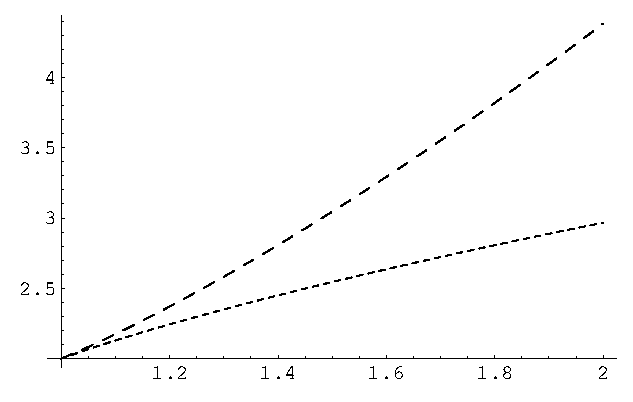
\includegraphics[width=0.4\textwidth]{cv/cv/twovals}
    \end{center}
    \caption{Values of the integral.}
    \label{twovals}
  \end{figure}

  Thus we see that 
  \[
  \boxed{
    \hat{y} = \frac{x^2}{4a} + a, \qquad
    a = \frac{1}{2} \left( y_1 + \sqrt{y_1^2 - x_1^2} \right)
    }
  \]
  is the extremal with the smaller integral and is the minimizing curve
  in $C^1$ for $y_1 \geq x^1$.  For $y_1 < x_1$ the $C^1$ extremum is,
  \[
  \boxed{ 
    \hat{y} = y_1.
    }
  \]






  \textbf{$\mathbf{C^1_p}$ Extremals.}
  Consider the parametric form of the Lagrangian.
  \[
  \int_{t_0}^{t_1} \sqrt{y(t)} \sqrt{(x'(t))^2 + (y'(t))^2}\,\dd t
  \]
  The Euler differential equations are
  \[
  \frac{\dd}{\dd t} f_{x'} - f_{x} = 0 \quad \mathrm{and} \quad
  \frac{\dd}{\dd t} f_{y'} - f_{y} = 0.
  \] 
  If one of the equations is satisfied, then the other is automatically 
  satisfied, (or the extremal is straight).  With either of these equations
  we could derive the quadratic extremal and the $y = \mathrm{const}$ extremal that
  we found previously.  We will find one more extremal by considering the
  first parametric Euler differential equation.
  \[
  \frac{\dd}{\dd t} f_{x'} - f_{x} = 0 
  \]
  \[
  \frac{\dd}{\dd t} \left( \frac{ \sqrt{y(t)} x'(t)}{\sqrt{(x'(t))^2 + (y'(t))^2}}
  \right) = 0
  \]
  \[
  \frac{ \sqrt{y(t)} x'(t)}{\sqrt{(x'(t))^2 + (y'(t))^2}} = \mathrm{const}
  \]
  Note that $x(t) = \mathrm{const}$ is a solution.
  Thus the extremals are of the three forms,
  \begin{align*}
    x &= \mathrm{const}, \\
    y &= \mathrm{const}, \\
    y &= \frac{x^2}{4a} + \frac{b x}{2 a} + \frac{b^2}{4a} + a.
  \end{align*}

  The Erdmann corner conditions require that
  \begin{gather*}
    F_{y'} = \frac{ \sqrt{y} y' }{ \sqrt{ 1 + (y')^2 } }, \\
    F - y' F_{y'} = \sqrt{y} \sqrt{1 + (y')^2}
    - \frac{ \sqrt{y} (y')^2 }{ \sqrt{ 1 + (y')^2 } }
    = \frac{ \sqrt{y} }{ \sqrt{ 1 + (y')^2 } }
  \end{gather*}
  are continuous at corners.  There can be corners only if $y = 0$.  

  Now we piece the three forms together to obtain $C^1_p$ extremals that
  satisfy the Erdmann corner conditions.  The only possibility that is not 
  $C^1$ is the extremal
  that is a horizontal line from $(0,0)$ to $(x_1,0)$ and then a vertical
  line from $(x_1,y_1)$.  The value of the integral for this extremal is
  \[
  \int_0^{y_1} \sqrt{t} \,\dd t = \frac{2}{3} (y_1)^{3/2}.
  \]
  Equating the performance indices of the quadratic extremum and the 
  piecewise smooth extremum,
  \[
  \frac{ x_1 (x_1^2 + 3( y_1 + \sqrt{y_1^2 - x_1^2} )^2 }
  { 3 \sqrt{2} ( y_1 + \sqrt{ y_1^2 - x_1^2} )^3 } = 
  \frac{2}{3} (y_1)^{3/2},
  \]
  \[
  y_1 = \pm x_1 \frac{ \sqrt{3 \pm 2 \sqrt{3}} }{ \sqrt{3} }.
  \]
  The only real positive solution is
  \[
  y_1 = x_1 \frac{ \sqrt{3 + 2 \sqrt{3}} }{ \sqrt{3} } \approx 1.46789\, x_1.
  \]
  The piecewise smooth extremal has the smaller performance index for 
  $y_1$ smaller than this value and the quadratic extremal has the smaller
  performance index for $y_1$ greater than this value.


  \begin{center}
    \fbox{
      \parbox{5.5in}{
        The $C^1_p$ extremum is the piecewise smooth extremal for 
        $y_1 \leq x_1 \sqrt{3 + 2 \sqrt{3}}/\sqrt{3}$ and is the quadratic extremal
        for $y_1 \geq x_1 \sqrt{3 + 2 \sqrt{3}}/\sqrt{3}$.
        }
      }
  \end{center}
\end{Solution}



%%A perfectly flexible uniform rope of length $L$ hangs in equilibrium 
\begin{Solution}
  The shape of the rope will be a catenary between $x_1$ and $x_2$ and be
  a vertically hanging segment after that.  Let the length of the 
  vertical segment be $z$.
  Without loss of generality we take $x_1 = y_2 = 0$.  The potential 
  energy, (relative to $y = 0$), of a length of rope $d s$ in $0 \leq x \leq x_2$
  is $m g y = \rho g y\,\dd s$.  The total potential energy of the 
  vertically hanging rope is $m (\mathrm{center of mass}) g = \rho z (-z/2) g$.
  Thus we seek to minimize,
  \[
  \rho g \int_0^{x_2} y \,\dd s - \frac{1}{2} \rho g z^2, \qquad
  y(0) = y_1, \quad y(x_2) = 0,
  \]
  subject to the isoperimetric constraint,
  \[
  \int_0^{x_2}\,\dd s - z = L.
  \]
  Writing the arc-length differential as $d s = \sqrt{1 + (y')^2}\,\dd x$ we 
  minimize
  \[
  \rho g \int_0^{x_2} y \sqrt{1 + (y')^2} \,\dd s - \frac{1}{2} \rho g z^2, \qquad
  y(0) = y_1, \quad y(x_2) = 0,
  \]
  subject to,
  \[
  \int_0^{x_2} \sqrt{1 + (y')^2} \,\dd x - z = L.
  \]



  Consider the more general problem of finding functions $y(x)$ and numbers
  $z$ which extremize $I \equiv \int_a^b F(x, y, y')\,\dd x + f(z)$ subject
  to $J \equiv \int_a^b G(x, y, y')\,\dd x + g(z) = L$.

  Suppose $y(x)$ and $z$ are the desired solutions and form the comparison
  families, $y(x) + \epsilon_1 \eta_1(x) + \epsilon_2 \eta_2(x)$, 
  $z + \epsilon_1 \zeta_1 + \epsilon_2 \zeta_2$.  Then, there exists a 
  constant such that
  \begin{align*}
    \frac{\partial}{\partial \epsilon_1} (I + \lambda J) \big|_{\epsilon_1,\epsilon_2=0} &= 0 \\
    \frac{\partial}{\partial \epsilon_2} (I + \lambda J) \big|_{\epsilon_1,\epsilon_2=0} &= 0.
  \end{align*}
  These equations are
  \[
  \int_a^b \left( \frac{\dd}{\dd x} H_{,y'} - H_y \right) \eta_1 \,\dd x
  + h'(z) \zeta_1 = 0,
  \]
  and
  \[
  \int_a^b \left( \frac{\dd}{\dd x} H_{,y'} - H_y \right) \eta_2 \,\dd x
  + h'(z) \zeta_2 = 0,
  \]
  where $H = F + \lambda G$ and $h = f + \lambda g$.  From this we conclude
  that
  \[
  \frac{\dd}{\dd x} H_{,y'} - H_y = 0, \qquad h'(z) = 0
  \]
  with $\lambda$ determined by 
  \[
  J = \int_a^b G(x,y,y')\,\dd x + g(z) = L.
  \]


  Now we apply these results to our problem.  Since 
  $f(z) =  - \frac{1}{2} \rho g z^2$ and
  $g(z) = - z$ we have
  \[
  - \rho g z - \lambda = 0,
  \]
  \[
  \boxed{
    z = - \frac{\lambda}{\rho g}.
    }
  \]
  It was shown in class that the solution of the Euler differential equation
  is a family of catenaries,
  \[
  y = - \frac{\lambda}{\rho g} + c_1 \cosh \left( \frac{x - c_2}{c_1} \right).
  \]
  One can find $c_1$ and $c_2$ in terms of $\lambda$ by applying the
  end conditions $y(0) = y_1$ and $y(x_2) = 0$.  Then the expression 
  for $y(x)$ and $z = - \lambda / \rho g$ are substituted into the 
  isoperimetric constraint to determine $\lambda$.


  Consider the special case that $(x_1,y_1) = (0,0)$ and $(x_2,y_2) = (1,0)$.
  In this case we can use the fact that $y(0) = y(1)$ to solve for $c_2$
  and write $y$ in the form
  \[
  y = - \frac{\lambda}{\rho g} + c_1 \cosh \left( \frac{x - 1/2}{c_1} \right).
  \]
  Applying the condition $y(0) = 0$ would give us the algebraic-transcendental
  equation,
  \[
  y(0) = - \frac{\lambda}{\rho g} + c_1 \cosh \left( \frac{1}{2 c_1} \right) = 0,
  \]
  which we can't solve in closed form.  
  Since we ran into a dead end in applying the boundary condition, we turn
  to the isoperimetric constraint.
  \[
  \int_0^1 \sqrt{1 + (y')^2}\,\dd x - z = L
  \]
  \[
  \int_0^1 \cosh\left( \frac{x-1/2}{c_1} \right)\,\dd x - z = L
  \]
  \[
  2 c_1 \sinh\left( \frac{1}{2 c_1} \right) - z = L
  \]
  With the isoperimetric constraint, the algebraic-transcendental equation and
  $z = - \lambda / \rho g$ we now have
  \begin{align*}
    z &= - c_1 \cosh \left( \frac{1}{2 c_1} \right), \\
    z &= 2 c_1 \sinh \left( \frac{1}{2 c_1} \right) - L.
  \end{align*}
  For any fixed $L$, we can numerically solve for $c_1$ and thus obtain $z$.
  You can derive that there are no solutions unless $L$ is greater than about
  1.9366.  If $L$ is smaller than this, the rope would slip off the pin.
  For $L = 2$, $c_1$ has the values $0.4265$ and $0.7524$.  The larger
  value of $c_1$ gives the smaller potential energy.  The position of
  the end of the rope is $z = -0.9248$.
\end{Solution}



%%The drag on a supersonic airfoil of chord $c$ and shape $y = y(x)$ is 
\begin{Solution}
  Using the method of Lagrange multipliers, we look for stationary values of
  $\int_0^c ((y')^2 + \lambda y^2 )\,\dd x$,
  \[
  \delta \int_0^c ((y')^2 + \lambda y^2 )\,\dd x = 0.
  \]
  The Euler differential equation is
  \[
  \frac{\dd}{\dd x} F_(,y') - F_{,y} = 0,
  \]
  \[
  \frac{\dd}{\dd x} (2 y') - 2 \lambda y = 0.
  \]
  Together with the homogeneous boundary conditions, we have the problem
  \[
  y'' - \lambda y = 0, \qquad y(0) = y(c) = 0,
  \]
  which has the solutions,
  \[
  \lambda_n = - \left( \frac{n \pi}{c} \right)^2, \qquad
  y_n = a_n \sin\left( \frac{n \pi x}{c} \right), \qquad n \in \mathbb{Z}^+.
  \]
  Now we determine the constants $a_n$ with the moment of inertia constraint.
  \[
  \int_0^c a_n^2 \sin^2 \left( \frac{ n \pi x}{c} \right) \,\dd x
  = \frac{c a_n^2 }{2} = A
  \]
  Thus we have the extremals,
  \[
  y_n = \sqrt{ \frac{2 A}{c} } \sin \left( \frac{n \pi x}{c} \right), 
  \qquad n \in \mathbb{Z}^+.
  \]
  The drag for these extremals is
  \[
  D = \frac{2 A}{c} \int_0^c \left( \frac{n \pi}{c} \right)^2
  \cos^2 \left( \frac{n \pi x}{c} \right) \,\dd x
  = \frac{A n^2 \pi^2}{c^2}.
  \]
  We see that the drag is minimum for $n = 1$.  The shape for minimum 
  drag is
  \[
  \boxed{
    \hat{y} = \sqrt{ \frac{2 A}{c} } \sin \left( \frac{n \pi x}{c} \right).
    }
  \]
\end{Solution}



%%The deflection $y$ of a beam executing free (small) vibrations of 
\begin{Solution}
  Consider the general problem of determining the stationary values of
  the quantity $\omega^2$ given by
  \[
  \omega^2 = \frac{ \int_a^b F(x, y, y', y'' )\,\dd x }
  { \int_a^b G(x, y, y', y'' )\,\dd x }
  \equiv \frac{I}{J}.
  \]
  The variation of $\omega^2$ is
  \begin{align*}
    \delta \omega^2 
    &= \frac{ J \delta I - I \delta J }{J^2} \\
    &= \frac{1}{J} \left( \delta I - \frac{I}{J} \delta J \right) \\
    &= \frac{1}{J} \left( \delta I - \omega^2 \delta J \right).
  \end{align*}
  The the values of $y$ and $y'$ are specified on the boundary, then the 
  variations of $I$ and $J$ are
  \[
  \delta I = \int_a^b \left( \frac{\dd^2}{\dd x^2} F_{,y''} - \frac{\dd}{\dd x} F_{,y'}
    + F_{,y} \right) \delta y \,\dd x, \qquad
  \delta J = \int_a^b \left( \frac{\dd^2}{\dd x^2} G_{,y''} - \frac{\dd}{\dd x} G_{,y'}
    + G_{,y} \right) \delta y \,\dd x
  \]
  Thus $\delta \omega^2 = 0$ becomes
  \[
  \frac{ \int_a^b \left( \frac{\dd^2}{\dd x^2} H_{,y''} - \frac{\dd}{\dd x} H_{,y'}
      + H_{,y} \right) \delta y \,\dd x }{ \int_a^b G \,\dd x } = 0,
  \]
  where $H = F - \omega^2 G$.  A necessary condition for an extremum is
  \[
  \boxed{
    \frac{\dd^2}{\dd x^2} H_{,y''} - \frac{\dd}{\dd x} H_{,y'} + H_{,y} = 0 \quad
    \mathrm{where}\ H \equiv F - \omega^2 G.
    }
  \]

  For our problem we have $F = E I (y'')^2$ and $G = \rho y$ so that 
  the extremals are solutions of
  \[
  \frac{\dd^2}{\dd x^2} \left( E I \frac{\dd y}{\dd x} \right) - \rho \omega^2 y = 0,
  \]
  With homogeneous boundary conditions we have an eigenvalue problem with
  deflections modes $y_n(x)$ and corresponding natural frequencies
  $\omega_n$.
\end{Solution}



%%A boatman wishes to steer his boat so as to minimize the transit time
\begin{Solution}
  We assume that $v_0 > w(x,y,t)$ so that the problem has a solution for 
  any end point.  The crossing time is
  \[
  T = \int_0^l \left( \dot{X}(t) \right)^{-1} \,\dd x
  = \frac{1}{v_0} \int_0^l \sec \alpha(t) \,\dd x.
  \]
  Note that
  \begin{align*}
    \frac{\dd y}{\dd x} 
    &= \frac{w + v_0 \sin \alpha}{v_0 \cos \alpha} \\
    &= \frac{w}{v_0} \sec \alpha + \tan \alpha \\
    &= \frac{w}{v_0} \sec \alpha + \sqrt{\sec^2 \alpha - 1 }.
  \end{align*}
  We solve this relation for $\sec \alpha$.
  \[
  \left( y' - \frac{w}{v_0} \sec \alpha \right)^2 = \sec^2 \alpha - 1
  \]
  \[
  (y')^2 - 2 \frac{w}{v_0} y' \sec \alpha + \frac{w^2}{v_0^2} \sec^2 \alpha
  = \sec^2 \alpha - 1
  \]
  \[
  (v_0^2 - w^2) \sec^2 \alpha + 2 v_0 w y' \sec \alpha - v_0^2 ((y')^2 + 1) = 0
  \]
  \[
  \sec \alpha = \frac{ - 2 v_0 w y' \pm \sqrt{ 4 v_0^2 w^2 (y')^2 +
      4 (v_0^2 - w^2) v_0^2 ((y')^2 + 1) } }{ 2 (v_0^2 - w^2) }
  \]
  \[
  \sec \alpha = v_0 \frac{ - w y' \pm \sqrt{ 
      v_0^2 ((y')^2 + 1)  - w^2 } }{ (v_0^2 - w^2) }
  \]
  Since the steering angle satisfies $-\pi/2 \leq \alpha \leq \pi/2$ only 
  the positive solution is relevant.
  \[
  \sec \alpha = v_0 \frac{ - w y' + \sqrt{ 
      v_0^2 ((y')^2 + 1)  - w^2 } }{ (v_0^2 - w^2) }
  \]

  \textbf{Time Independent Current.}
  If we make the assumption that $w = w(x,y)$ then we can write the 
  crossing time as an integral of a function of $x$ and $y$.  
  \[
  T(y) = \int_0^l \frac{ - w y' + \sqrt{ 
      v_0^2 ((y')^2 + 1)  - w^2 } }{ (v_0^2 - w^2) } \,\dd x
  \]
  A necessary condition for a minimum is $\delta T = 0$.  The Euler differential
  equation for this problem is
  \[
  \frac{\dd}{\dd x} F_{,y'} - F_{,y} = 0
  \]
  \begin{multline*}
    \frac{\dd}{\dd x} \left( \frac{1}{v_0^2 - w^2} 
      \left( - w + \frac{v_0^2 y'}{\sqrt{ v_0^2 ((y')^2 + 1) - w^2 }} \right)
    \right)
    \\
    - \frac{w_y}{(v_0^2 - w^2)^2} \left( 
      \frac{ w (v^2 (1 + 2 (y')^2) - w^2 ) }{ \sqrt{v_0^2 ((y')^2+1) - w^2 } }
      - y' (v_0^2 + w^2 ) \right)
  \end{multline*}
  By solving this second order differential equation subject to the boundary
  conditions $y(0) = 0$, $y(l) = y_1$ we obtain the path of minimum crossing
  time.

  \textbf{Current $\mathbf{w = w(x)}$.}
  If the current is only a function of $x$, then the Euler differential
  equation can be integrated to obtain,
  \[
  \frac{1}{v_0^2 - w^2} 
  \left( - w + \frac{v_0^2 y'}{\sqrt{ v_0^2 ((y')^2 + 1) - w^2 }} \right)
  = c_0.
  \]
  Solving for $y'$, 
  \[
  y' = \pm \frac{w + c_0 ( v_0^2 - w^2 ) }
  { v_0 \sqrt{ 1 - 2 c_0 w - c_0^2 (v_0^2 - w^2 ) } }.
  \]
  Since $y(0) = 0$, we have
  \[
  \boxed{
    y(x) = \pm \int_0^x \frac{w(\xi) + c_0 ( v_0^2 - (w(\xi))^2 ) }
    { v_0 \sqrt{ 1 - 2 c_0 w(\xi) - c_0^2 (v_0^2 - (w(\xi))^2 ) } }.
    }
  \]
  For any given $w(x)$ we can use the condition $y(l) = y_1$ to solve for 
  the constant $c_0$.


  \textbf{Constant Current.}
  If the current is constant then the Lagrangian is a function of $y'$ alone.
  The admissible extremals are straight lines.  The solution is then
  \[
  \boxed{
    y(x) = \frac{y_1 x}{l}.
    }
  \]
\end{Solution}



%%Two particles of equal mass $m$ are connected by an inextensible string
\begin{Solution}
  \begin{enumerate}
    %%
    %%
    %%
  \item
    The kinetic energy of the first particle is 
    $\frac{1}{2} m ((\alpha - x) \hat{\theta} )^2$.  Its potential energy, relative
    to the table top, is zero.  The kinetic energy of the second particle is
    $\frac{1}{2} m \hat{x}^2$.  Its potential energy, relative to its equilibrium
    position is $-m g x$.  The Lagrangian is the difference of kinetic and 
    potential energy.
    \[
    \boxed{
      L = m \left( \dot{x}^2 + \frac{1}{2} (\alpha - x)^2 \dot{\theta}^2 + g x
      \right)
      }
    \]
    The Euler differential equations are the equations of motion.
    \[
    \frac{\dd}{\dd t} L_{,\dot{x}} - L_x = 0, \qquad
    \frac{\dd}{\dd t} L_{,\dot{\theta}} - L_\theta = 0
    \]
    \[
    \frac{\dd}{\dd t} ( 2 m \dot{x} ) + m (\alpha - x) \dot{\theta}^2 - m g = 0, 
    \qquad
    \frac{\dd}{\dd t} \left( m (\alpha - x)^2 \dot{\theta}^2 \right) = 0
    \]
    \[
    2 \ddot{x} + (\alpha - x) \dot{\theta}^2 - g = 0, 
    \qquad
    (\alpha - x)^2 \dot{\theta}^2 = \mathrm{const}
    \]
    When $x =0$, $\dot{\theta} = \omega = \sqrt{g/\alpha}$.  This determines the
    constant in the equation of motion for $\theta$.
    \[
    \boxed{
      \dot{\theta} = \frac{ \alpha \sqrt{\alpha g} }{ (\alpha - x)^2 }
      }
    \]
    Now we substitute the expression for $\dot{\theta}$ into the equation of
    motion for $x$.
    \[
    2 \ddot{x} + (\alpha - x) \frac{\alpha^3 g}{(\alpha-x)^4} - g = 0
    \]
    \[
    2 \ddot{x} + \left( \frac{\alpha^3}{(\alpha-x)^3} - 1 \right) g = 0
    \]
    \[
    \boxed{
      2 \ddot{x} + \left( \frac{1}{(1-x/\alpha)^3} - 1 \right) g = 0
      }
    \]
    %%
    %%
    %%
  \item
    For small oscillations, $\left| \frac{x}{\alpha} \right| \ll 1$.  Recall
    the binomial expansion,
    \[
    (1 + z)^a = \sum_{n = 0}^\infty \binom{a}{n} z^n, \quad \mathrm{for}\ |z| < 1,
    \]
    \[
    (1 + z)^a \approx 1 + a z, \quad \mathrm{for}\ |z| \ll 1.
    \]
    We make the approximation,
    \[
    \frac{1}{(1 - x/\alpha)^3} \approx 1 + 3 \frac{x}{\alpha},
    \]
    to obtain the linearized equation of motion,
    \[
    2 \ddot{x} + \frac{3 g}{\alpha} x = 0.
    \]
    This is the equation of a harmonic oscillator with solution
    \[
    x = a \sin \left( \sqrt{3 g}{2 \alpha} (t - b) \right).
    \]
    The period of oscillation is,
    \[
    \boxed{
      T = 2 \pi \sqrt{2 \alpha}{3 g}.
      }
    \]
  \end{enumerate}
\end{Solution}



%%A rocket is propelled vertically upward so as to reach a prescribed height
\begin{Solution}
  We write the equation of motion and boundary conditions,
  \[
  \ddot{x} = U(t) - g, \qquad x(0) = \dot{x}(0) = 0, \quad x(T) = h,
  \]
  as the first order system,
  \begin{alignat*}{3}
    \dot{x} &= 0, &\quad x(0) &= 0, &\quad x(T) &= h, \\
    \dot{y} &= U(t) - g, &\quad y(0) &= 0. &\quad &
  \end{alignat*}
  We seek to minimize,
  \[
  T = \int_0^T \,\dd t,
  \]
  subject to the constraints,
  \begin{align*}
    &\dot{x} - y = 0, \\
    &\dot{y} - U(t) + g = 0, \\
    &\int_0^T U^2(t)\,\dd t = k^2.
  \end{align*}
  Thus we seek extrema of
  \[
  \int_0^T H\,\dd t \equiv
  \int_0^T \left( 1 + \lambda(t) (\dot{x} - y) + \mu(t) (\dot{y} - U(t) + g)
    + \nu U^2(t) \right) \,\dd t.
  \]
  Since $y$ is not specified at $t = T$, we have the natural boundary condition,
  \[
  H_{,\dot{y}} \big|_{t=T} = 0,
  \]
  \[
  \mu(T) = 0.
  \]
  The first Euler differential equation is
  \[
  \frac{\dd}{\dd t} H_{,\dot{x}} - H_{,x} = 0,
  \]
  \[
  \frac{\dd}{\dd t} \lambda(t) = 0.
  \]
  We see that $\lambda(t) = \lambda$ is constant.
  The next Euler DE is
  \[
  \frac{\dd}{\dd t} H_{,\dot{y}} - H_{,y} = 0,
  \]
  \[
  \frac{\dd}{\dd t} \mu(t) + \lambda = 0.
  \]
  \[
  \mu(t) = - \lambda t + \mathrm{const}
  \]
  With the natural boundary condition, $\mu(T) = 0$, we have
  \[
  \mu(t) = \lambda (T - t).
  \]
  The final Euler DE is,
  \[
  \frac{\dd}{\dd t} H_{,\dot{U}} - H_{,U} = 0,
  \]
  \[
  \mu(t) - 2 \nu U(t) = 0.
  \]
  Thus we have
  \[
  U(t) =  \frac{ \lambda (T - t) }{2 \nu }.
  \]
  This is the required thrust function.  We use the constraints to find
  $\lambda$, $\nu$ and $T$.

  Substituting $U(t) = \lambda (T - t) / (2 \nu)$ into the isoperimetric 
  constraint, $\int_0^T U^2(t)\,\dd t = k^2$ yields
  \[
  \frac{ \lambda^2 T^3 }{ 12 \nu^2 } = k^2,
  \]
  \[
  \boxed{
    U(t) = \frac{ \sqrt{3} k }{ T^{3/2} } (T - t).
    }
  \]
  The equation of motion for $x$ is
  \[
  \ddot{x} = U(t) - g = \frac{ \sqrt{3} k }{ T^{3/2} } (T - t).
  \]
  Integrating and applying the initial conditions $x(0) = \dot{x}(0) = 0$
  yields,
  \[
  x(t) = \frac{ k t^2 (3 T - t) }{ 2 \sqrt{3} T^{3/2} } - \frac{1}{2} g t^2.
  \]
  Applying the condition $x(T) = h$ gives us,
  \[
  \frac{ k }{ \sqrt{3} } T^{3/2} - \frac{1}{2} g T^2 = h,
  \]
  \[
  \boxed{
    \frac{1}{4} g^2 T^4  - \frac{k}{3} T^3 + g h T^2 + h^2 = 0.
    }
  \]
  If $k \geq 4 \sqrt{2/3} g^{3/2} \sqrt{h}$ then this fourth degree polynomial 
  has positive, real solutions for $T$.  With strict inequality, the minimum
  time is the smaller of the two positive, real solutions.
  If $k < 4 \sqrt{2/3} g^{3/2} \sqrt{h}$ then there is not enough fuel to
  reach the target height.
\end{Solution}



%%A space vehicle moves along a straight path in free space.  $x(t)$ is
\begin{Solution}
  We have $\ddot{x} = U(t)$ where $U(t)$ is the acceleration furnished by
  the thrust of the vehicles engine.  In practice, the engine will be designed
  to operate within certain bounds, say $-M \leq U(t) \leq M$, where
  $\pm M$ is the maximum forward/backward acceleration.  To account for the
  inequality constraint we write $U = M \sin V(t)$ for some suitable $V(t)$.
  More generally, if we had $\phi(t) \leq U(t) \leq \psi(t)$, we could write
  this as $U(t) = \frac{\psi + \phi}{2} + \frac{\psi - \phi}{2} \sin V(t)$.

  We write the equation of motion as a first order system,
  \begin{alignat*}{3}
    \dot{x} &= y, &\quad x(0) &= a, &\quad x(T) &= 0, \\
    \dot{y} &= M \sin V, &\quad y(0) &= b, &\quad y(T) = 0.
  \end{alignat*}
  Thus we minimize
  \[
  T = \int_0^T \,\dd t
  \]
  subject to the constraints,
  \begin{align*}
    \dot{x} - y &= 0 \\
    \dot{y} - M \sin V &= 0.
  \end{align*}
  Consider
  \[
  H = 1 + \lambda(t) (\dot{x} - y) + \mu(t) (\dot{y} - M \sin V).
  \]
  The Euler differential equations are
  \begin{alignat*}{3}
    &\frac{\dd}{\dd t} H_{,\dot{x}} - H_{,x} = 0 &\quad \Rightarrow \quad
    &\frac{\dd}{\dd t} \lambda(t) = 0 &\quad \Rightarrow \quad
    &\lambda(t) = \mathrm{const} \\
    &\frac{\dd}{\dd t} H_{,\dot{y}} - H_{,y} = 0 &\quad \Rightarrow \quad
    &\frac{\dd}{\dd t} \mu(t) + \lambda = 0 &\quad \Rightarrow \quad
    &\mu(t) = - \lambda t + \mathrm{const} \\
    &\frac{\dd}{\dd t} H_{,\dot{V}} - H_{,V} = 0 &\quad \Rightarrow \quad
    &\mu(t) M \cos V(t) = 0 &\quad \Rightarrow \quad
    &V(t) = \frac{\pi}{2} + n \pi.
  \end{alignat*}
  Thus we see that 
  \[
  U(t) = M \sin \left( \frac{\pi}{2} + n \pi \right) = \pm M.
  \]

  Therefore, if the rocket is to be transferred from its initial state to is
  specified final state in minimum time with a limited source of thrust, 
  ($|U| \leq M$), then the engine should operate at full power at all times
  except possibly for a finite number of switching times.  (Indeed, if some
  power were not being used, we would expect the transfer would be speeded 
  up by using the additional power suitably.)

  To see how this "bang-bang" process works, we'll look at the phase plane.
  The problem
  \begin{alignat*}{2}
    \dot{x} &= y, &\quad x(0) &= c, \\
    \dot{y} &= \pm M, &\quad y(0) &= d,
  \end{alignat*}
  has the solution
  \[
  x(t) = c + d t \pm M \frac{t^2}{2}, \qquad
  y(t) = d \pm M t.
  \]
  We can eliminate $t$ to get
  \[
  x = \pm \frac{y^2}{2 M} + c \mp \frac{d^2}{2 M}.
  \]
  These curves are plotted in Figure~\ref{hw4p3p1}.

  \begin{figure}[h!]
    \begin{center}
      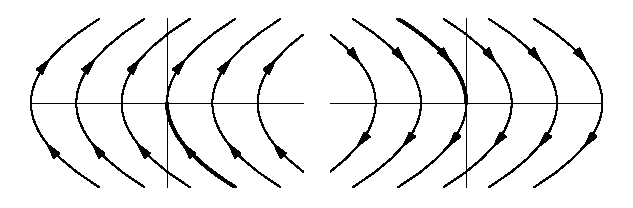
\includegraphics[width=\textwidth]{cv/cv/hw4p3p1}
    \end{center}
    \caption{The trajectories.}
    \label{hw4p3p1}
  \end{figure}

  There is only curve in each case which transfers the initial state to 
  the origin.  We will denote these curves $\gamma$ and $\Gamma$, respectively.
  Only if the initial point $(a,b)$ lies on one of these two curves can we 
  transfer the state of the system to the origin along an extremal without
  switching.  If $a = \frac{b^2}{2M}$ and $b < 0$ then this is possible using
  $U(t) = M$.  If $a = - \frac{b^2}{2M}$ and $b > 0$ then this is possible 
  using $U(t) = - M$.  Otherwise we follow an extremal that intersects the
  initial position until this curve intersects $\gamma$ or $\Gamma$.  We then
  follow $\gamma$ or $\Gamma$ to the origin.
\end{Solution}



%%$I(y) = \int_0^m \sqrt{y + h} \sqrt{1 + (y')^2 } \,\dd x$
\begin{Solution}
  Since the integrand does not explicitly depend on $x$, the Euler differential
  equation has the first integral,
  \[
  F - y' F_{y'} = \mathrm{const}.
  \]
  \[
  \sqrt{y+h} \sqrt{1+(y')^2} - y' \frac{y' \sqrt{y+h}}{\sqrt{1+(y')^2}}
  = \mathrm{const}
  \]
  \[
  \frac{\sqrt{y+h}}{\sqrt{1+(y')^2}} = \mathrm{const}
  \]
  \[
  y + h = c_1^2 (1 + (y')^2)
  \]
  \[
  \sqrt{ y + h - c_1^2 } = c_1 y'
  \]
  \[
  \frac{ c_1 \,\dd y }{ \sqrt{ y + h - c_1^2 } } = d x
  \]
  \[
  2 c_1 \sqrt{ y + h - c_1^2 } = x - c_2
  \]
  \[
  4 c_1^2 ( y + h - c_1^2 ) = (x - c_2)^2
  \]
  Since the extremal passes through the origin, we have
  \[
  4 c_1^2 ( h - c_1^2 ) = c_2^2.
  \]
  \begin{equation}
    \label{1_1}
    4 c_1^2  y  = x^2 - 2 c_2 x
  \end{equation}
  Introduce as a parameter the slope of the extremal at the origin; that is,
  $y'(0) = \alpha$.  Then differentiating (\ref{1_1}) at $x = 0$ yields
  $4 c_1^2 \alpha = - 2 c_2$.  Together with $c_2^2 = 4 c_1^2 (h - c_1^2)$
  we obtain $c_1^2 = \frac{h}{1+\alpha^2}$ and 
  $c_2 = - \frac{2 \alpha h}{1 + \alpha^2}$.
  Thus the equation of the pencil (\ref{1_1}) will have the form
  \begin{equation}
    \label{1_2}
    y = \alpha x + \frac{1 + \alpha^2}{4 h} x^2.
  \end{equation}
  To find the envelope of this family we differentiate (~\ref{1_2}) with
  respect to $\alpha$ to obtain $0 = x + \frac{\alpha}{2h} x^2$ and
  eliminate $\alpha$ between this and (~\ref{1_2}) to obtain
  \[
  y = -h + \frac{x^2}{4h}.
  \]
  See Figure~\ref{parasafe} for a plot of some extremals and the envelope.


  \begin{figure}[h!]
    \begin{center}
      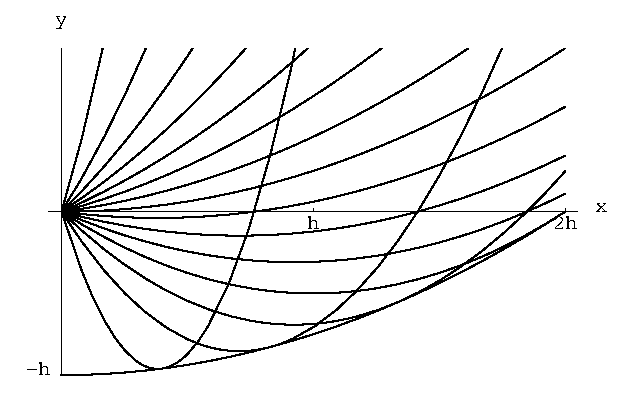
\includegraphics[width=0.5\textwidth]{cv/cv/parasafe}
    \end{center}
    \caption{Some extremals and the envelope.}
    \label{parasafe}
  \end{figure}


  All extremals (\ref{1_2}) lie above the envelope which in ballistics is
  called the parabola of safety.  If $(m,M)$ lies outside the parabola,
  $M < -h + \frac{m^2}{4h}$, then it cannot be joined to $(0,0)$ by
  an extremal.  If $(m,M)$ is above the envelope then there are two candidates.
  Clearly we rule out the one that touches the envelope because of the
  occurrence of conjugate points.  For the other extremal, problem 2 
  shows that $E \geq 0$ for all $y'$.  Clearly we can embed this extremal in
  an extremal pencil, so Jacobi's test is satisfied.  Therefore the
  parabola that does not touch the envelope is a strong minimum.
\end{Solution}



%%Show that for the functional $\int n(x,y) \sqrt{1+(y')^2} \,\dd x$,
\begin{Solution}
  \begin{align*}
    E       &= F(x,y,y') - F(x,y,p) - (y'-p) F_{y'}(x,y,p) \\
    &= n \sqrt{1+(y')^2} - n \sqrt{1 + p^2} - (y'-p) 
    \frac{ n p }{ \sqrt{1 + p^2} } \\
    &= \frac{n}{\sqrt{1+p^2}} \left( \sqrt{1+(y')^2} \sqrt{1+p^2}
      - (1+p^2) - (y'-p)p \right) \\
    &= \frac{n}{\sqrt{1+p^2}} \left( \sqrt{ 1 + (y')^2 + p^2 + (y')^2 p^2
        - 2 y' p + 2 y' p } - (1 + p y' ) \right) \\
    &= \frac{n}{\sqrt{1+p^2}} \left( \sqrt{ (1+p y')^2 + (y'-p)^2 }
      - (1 + p y' ) \right) \\
    &\geq 0
  \end{align*}


  The speed of light in an inhomogeneous medium is 
  $\frac{\dd s}{\dd t} = \frac{1}{n(x,y}$.  The time of transit is then
  \[
  T = \int_{(a,A)}^{(b,B)} \frac{\dd t}{\dd s} \,\dd s 
  = \int_a^b n(x,y) \sqrt{1 + (y')^2} \,\dd x.
  \]
  Since $E \geq 0$, light traveling on extremals follow the time optimal path
  as long as the extremals do not intersect.
\end{Solution}



%%Consider the integral $\int \frac{1 + y^2}{(y')^2} \,\dd x$ between fixed
\begin{Solution}
  \textbf{Extremals.}
  Since the integrand does not depend explicitly on $x$, the Euler differential
  equation has the first integral,
  \[
  F - y' F_{,y'} = \mathrm{const}.
  \]
  \[
  \frac{1 + y^2}{(y')^2} - y' \frac{-2(1 + y^2)}{(y')^3} = \mathrm{const}
  \]
  \[
  \frac{d y}{\sqrt{1 + (y')^2}} = \mathrm{const} \,\dd x
  \]
  \[
  \arcsinh( y ) = c_1 x + c_2
  \]
  \[
  \boxed{
    y = \sinh( c_1 x + c_2 )
    }
  \]


  \textbf{Jacobi Test.}
  We can see by inspection that no conjugate points exist.  Consider the
  central field through $(0,0)$, $\sinh(c x)$, (See Figure~\ref{sinh}).

  \begin{figure}[h!]
    \begin{center}
      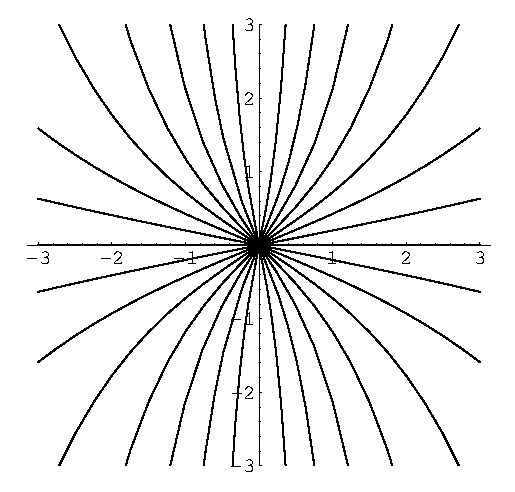
\includegraphics[width=0.4\textwidth]{cv/cv/sinh}
    \end{center}
    \caption{The hyperbolic sine for various values of the constant.}
    \label{sinh}
  \end{figure}

  We can also easily arrive at this conclusion analytically as follows:
  Solutions $u_1$ and $u_2$ of the Jacobi equation are given by
  \begin{align*}
    u_1 &= \frac{\partial y}{\partial c_2} = \cosh(c_1 x + c_2), \\
    u_2 &= \frac{\partial y}{\partial c_1} = x \cosh(c_1 x + c_2).
  \end{align*}
  Since $u_2 / u_1 = x$ is monotone for all $x$ there are no conjugate points.




  \textbf{Weierstrass Test.}
  \begin{align*}
    E       &= F(x,y,y') - F(x,y,p) - (y'-p) F_{,y'}(x,y,p) \\
    &= \frac{ 1 + y^2 }{ (y')^2 } - \frac{ 1 + y^2 }{ p^2 }
    - (y' - p) \frac{-2 (1 + y^2) }{ p^3 } \\
    &= \frac{ 1 + y^2 }{ (y')^2 p^2 } \left(
      \frac{ p^3 - p (y')^2 + 2 (y')^3 - 2 p (y')^2 }{ p } \right)\\
    &= \frac{ 1 + y^2 }{ (y')^2 p^2 } \left(
      \frac{ (p - y')^2 (p + 2 y') }{ p } \right)
  \end{align*}
  For $p = p(x,y)$ bounded away from zero, $E$ is one-signed for values of
  $y'$ close to $p$.  However, since the factor $(p + 2y')$ can have any
  sign for arbitrary values of $y'$, the conditions for a strong minimum
  are not satisfied.

  Furthermore, since the extremals are $y = \sinh(c_1 x + c_2)$, the slope
  function $p(x,y)$ will be of one sign only if the range of integration
  is such that we are on a monotonic piece of the $\sinh$.  If 
  we span both an increasing and decreasing section, $E$ changes
  sign even for weak variations.





  \textbf{Legendre Condition.}
  \[
  F_{,y'y'} = \frac{ 6 (1 + y^2) }{ (y')^4 } > 0
  \]
  Note that $F$ cannot be represented in a Taylor series for arbitrary values
  of $y'$ due to the presence of a discontinuity in $F$ when $y' = 0$.
  However, $F_{,y'y'} > 0$ on an extremal implies a weak minimum is provided
  by the extremal.


  \textbf{Strong Variations.}
  Consider $\int \frac{ 1 + y^2 }{ (y')^2 } \,\dd x$ on both an extremal and on 
  the special piecewise continuous variation in the figure.  On $PQ$ we 
  have $y' = \infty$ with implies that $\frac{ 1 + y^2 }{ (y')^2 } = 0$
  so that there is no contribution to the integral from $PQ$.

  On $QR$ the value of $y'$ is greater than its value along the extremal 
  $PR$ while the value of $y$ on $QR$ is less than the value of $y$ along
  $PR$.  Thus on $QR$ the quantity $\frac{ 1 + y^2 }{ (y')^2 }$ is less 
  than it is on the extremal $PR$.
  \[
  \int_{QR} \frac{ 1 + y^2 }{ (y')^2 } \,\dd x <
  \int_{PR} \frac{ 1 + y^2 }{ (y')^2 } \,\dd x
  \]
  Thus the weak minimum along the extremal can be weakened by a strong 
  variation.
\end{Solution}



%%Consider $I = \int_{x_0}^{x_1} y' (1 + x^2 y') \,\dd x$, $y(x_0) = y_0$,
\begin{Solution}
  The Euler differential equation is
  \[
  \frac{\dd}{\dd x} F_{,y'} - F_{,y} = 0.
  \]
  \[
  \frac{\dd}{\dd x} (1 + 2 x^2 y') = 0
  \]
  \[
  1 + 2 x^2 y' = \mathrm{const}
  \]
  \[
  y' = \mathrm{const} \frac{1}{x^2}
  \]
  \[
  \boxed{
    y = \frac{c_1}{x} + c_2
    }
  \]
  \begin{itemize}
  \item[(i)]
    No continuous extremal exists in $-1 \leq x \leq 2$ that satisfies 
    $y(-1) = 1$ and $y(2) = 4$.
  \item[(ii)]
    The continuous extremal that satisfies the boundary conditions is 
    $y = 7 - \frac{4}{x}$. Since $F_{,y'y'} = 2 x^2 \geq 0$ has a Taylor series
    representation for all $y'$, this extremal provides a strong minimum.
  \item[(iii)]
    The continuous extremal that satisfies the boundary conditions is 
    $y = 1$.  This is a strong minimum.
  \end{itemize}
\end{Solution}



%%\iint_D (Q_x - P_y) \,\dd x\,\dd y = \int_\Gamma (P \,\dd x + Q\,\dd y)
\begin{Solution}
  For identity (a) we take $P = 0$ and $Q = \phi \psi_x - \psi \phi_x$.
  For identity (b) we take $P = \phi \psi_y - \psi \phi_y$ and $Q = 0$.
  For identity (c) we take $P = - \frac{1}{2} (\phi \psi_x - \psi \phi_x )$
  and $Q = \frac{1}{2} (\phi \psi_y - \psi \phi_y)$.
  \[
  \iint_D \left( \frac{1}{2} (\phi \psi_y - \psi \phi_y)_x
    - \left( - \frac{1}{2} \right) (\phi \psi_x - \psi \phi_x)_y \right)
  \,\dd x\,\dd y
  = \int_\Gamma \left( - \frac{1}{2} (\phi \psi_x - \psi \phi_x )\,\dd x
    + \frac{1}{2} (\phi \psi_y - \psi \phi_y) \,\dd y \right)
  \]
  \begin{align*}
    &\iint_D \left( \frac{1}{2} (\phi_x \psi_y + \phi \psi_{x y} 
      - \psi_x \phi_y - \psi \phi_{x y})
      + \frac{1}{2} (\phi_y \psi_x \phi \psi_{x y} 
      - \psi_y \phi_x - \psi \phi_{x y} ) \right)
    \,\dd x\,\dd y \\
    &\qquad\qquad
    = - \frac{1}{2} \int_\Gamma (\phi \psi_x - \psi \phi_x ) \,\dd x 
    + \frac{1}{2} \int_\Gamma (\phi \psi_y - \psi \phi_y ) \,\dd y 
  \end{align*}
  \[
  \iint_D \phi \psi_{x y} \,\dd x \,\dd y
  = \iint_D \psi \phi_{x y} \,\dd x \,\dd y
  - \frac{1}{2} \int_\Gamma (\phi \psi_x - \psi \phi_x ) \,\dd x 
  + \frac{1}{2} \int_\Gamma (\phi \psi_y - \psi \phi_y ) \,\dd y
  \]


  The variation of $I$ is
  \[
  \delta I = \int_{t_0}^{t_1} \iint_D \left( -2 (u_{x x} + u_{y y})
    ( \delta u_{x x} + \delta u_{y y} ) + 2 (1 - \mu) 
    ( u_{x x} \delta u_{y y} + u_{y y} \delta u_{x x} 
    - 2 u_{x y} \delta u_{x y} ) \right) \,\dd x\,\dd y\,\dd t.
  \]
  From (a) we have
  \begin{align*}
    \iint_D -2 (u_{x x} + u_{y y}) \delta u_{x x} \,\dd x\,\dd y
    &= \iint_D -2 (u_{x x} + u_{y y})_{x x} \delta u \,\dd x\,\dd y \\
    &\qquad\qquad + \int_\Gamma -2 ( (u_{x x} + u_{y y}) \delta u_x
    - (u_{x x} + u_{y y})_x \delta u ) \,\dd y.
  \end{align*}
  From (b) we have
  \begin{align*}
    \iint_D -2 (u_{x x} + u_{y y}) \delta u_{y y} \,\dd x\,\dd y
    &= \iint_D -2 (u_{x x} + u_{y y})_{y y} \delta u \,\dd x\,\dd y \\
    &\qquad \qquad - \int_\Gamma -2 ( (u_{x x} + u_{y y}) \delta u_y
    - (u_{x x} + u_{y y})_y \delta u ) \,\dd y.
  \end{align*}
  From (a) and (b) we get
  \begin{align*}
    &\iint_D 2 (1 - \mu) (u_{x x} \delta u_{y y} + u_{y y} \delta u_{x x} )
    \,\dd x\,\dd y \\
    &\qquad \qquad
    = \iint_D 2 (1 - \mu) (u_{x x y y} + u_{y y x x}) \delta u \,\dd x\,\dd y \\
    &\qquad\qquad\qquad
    + \int_\Gamma 2 (1 - \mu) ( -( u_{x x} \delta u_y - u_{x x y} \delta u )\,\dd x
    + (u_{y y} \delta u_x - u_{y y x} \delta u )\,\dd y ).
  \end{align*}
  Using $c$ gives us
  \begin{align*}
    \iint_D 2 (1 - \mu) ( -2 u_{x y} \delta u_{x y} ) \,\dd x\,\dd y
    &= \iint_D 2 (1 - \mu) (-2 u_{x y x y} \delta u) \,\dd x\,\dd y \\
    &\qquad
    + \int_\Gamma 2 (1 - \mu) ( u_{x y} \delta u_x - u_{x y x} \delta u)\,\dd x \\
    &\qquad
    - \int_\Gamma 2 (1 - \mu) ( u_{x y} \delta u_y - u_{x y y} \delta u)\,\dd y.
  \end{align*}
  Note that
  \[
  \frac{\partial u}{\partial n} \,\dd s = u_x \,\dd y - u_y \,\dd x.
  \]
  Using the above results, we obtain
  \begin{align*}
    \delta I
    &= 2 \int_{t_0}^{t_1} \iint_D (- \nabla^4 u )\delta u\,\dd x\,\dd y\,\dd t
    + 2 \int_{t_0}^{t_1} \int_\Gamma \left( \frac{\partial (\nabla^2 u)}{\partial n}
      \delta u + (\nabla^2 u) \frac{\partial (\delta u)}{\partial n} \right)\,\dd s\,\dd t \\
    &\qquad + 2 (1-\mu) \int_{t_0}^{t_1} \left( \int_\Gamma
      (u_{y y} \delta u_x - u_{x y} \delta u_y )\,\dd y
      + (u_{x y} \delta u_x - u_{x x} \delta u_y)\,\dd x \right) \,\dd t.
  \end{align*}
\end{Solution}



%%For the following functionals use the Rayleigh-Ritz method to find an 
\begin{Solution}
  \begin{enumerate}
    %%
    %%
    %%
  \item
    \textbf{Exact Solution.}
    The Euler differential equation is
    \begin{gather*}
      \frac{\dd}{\dd x} F_{,y'} = F_{,y} \\
      \frac{\dd}{\dd x} [2 y'] = -2 y - 2 x \\
      y'' + y = - x. \\
      \intertext{The general solution is}
      y = c_1 \cos x + c_2 \sin x - x. \\
      \intertext{Applying the boundary conditions we obtain,}
      \boxed{
        y = \frac{\sin x}{\sin 1} - x.
        } 
    \end{gather*}
    The value of the integral for this extremal is
    \[
    \boxed{
      J \left[ \frac{\sin x}{\sin 1} - x \right]
      = \cot(1) - \frac{2}{3} 
      \approx -0.0245741.
      }
    \]




    \textbf{$\mathbf{n \boldsymbol{=} 0}$.}
    We consider an approximate solution of the form $y(x) = a x (1-x)$.  We 
    substitute this into the functional.
    \[
    J(a) = \int_0^1 \left( (y')^2 - y^2 - 2 x y \right) \,\dd x  
    = \frac{3}{10} a^2 - \frac{1}{6} a 
    \]
    The only stationary point is
    \begin{gather*}
      J'(a) = \frac{3}{5} a - \frac{1}{6} = 0 \\
      a = \frac{5}{18}.
    \end{gather*}
    Since
    \[
    J''\left( \frac{5}{18} \right) = \frac{3}{5} > 0,
    \]
    we see that this point is a minimum.
    The approximate solution is
    \[
    \boxed{
      y(x) = \frac{5}{18} x (1-x).
      }
    \]
    This one term approximation and the exact solution are plotted in 
    Figure~\ref{p1_1t}.  The value of the functional is
    \[
    \boxed{
      J = - \frac{5}{216} \approx -0.0231481.
      }
    \]

    \begin{figure}[h!]
      \begin{center}
        \includegraphics[width=0.4\textwidth]{cv/cv/p1_1t}
      \end{center}
      \caption{One term approximation and exact solution.}
      \label{p1_1t}
    \end{figure}





    \textbf{$\mathbf{n \boldsymbol{=} 1}$.}
    We consider an approximate solution of the form $y(x) = x (1-x)( a + b x )$.  
    We substitute this into the functional.
    \[
    J(a,b) = \int_0^1 \left( (y')^2 - y^2 - 2 x y \right) \,\dd x  
    = \frac{1}{210} \left( 63 a^2 + 63 a b + 26 b^2 - 35 a - 21 b \right)
    \]
    We find the stationary points.
    \begin{align*}
      J_a &= \frac{1}{30} (18 a + 9 b - 5) = 0 \\
      J_b &= \frac{1}{210} (63 a + 52 b - 21) = 0
    \end{align*}
    \[
    a = \frac{71}{369}, \quad b = \frac{7}{41}
    \]
    Since the Hessian matrix
    \[
    H = 
    \begin{pmatrix}
      J_{a a} & J_{a b} \\
      J_{b a} & J_{b b}
    \end{pmatrix}
    =
    \begin{pmatrix}
      \frac{3}{5} & \frac{3}{10} \\
      \frac{3}{10} & \frac{26}{105}
    \end{pmatrix},
    \]
    is positive definite,
    \[
    \frac{3}{5} > 0, \quad \det(H) = \frac{41}{700},
    \]
    we see that this point is a minimum.  The approximate solution is
    \[
    \boxed{
      y(x) = x (1-x) \left( \frac{71}{369} + \frac{7}{41} x \right).
      }
    \]
    This two term approximation and the exact solution are plotted in 
    Figure~\ref{p1_2t}.  The value of the functional is
    \[
    \boxed{
      J = - \frac{136}{5535} \approx -0.0245709.
      }
    \]


    \begin{figure}[h!]
      \begin{center}
        \includegraphics[width=0.4\textwidth]{cv/cv/p1_2t}
      \end{center}
      \caption{Two term approximation and exact solution.}
      \label{p1_2t}
    \end{figure}
    %%
    %%
    %%
  \item
    \textbf{Exact Solution.}
    The Euler differential equation is
    \begin{gather*}
      \frac{\dd}{\dd x} F_{,y'} = F_{,y} \\
      \frac{\dd}{\dd x} [2 y'] = 2 y + 2 x \\
      y'' - y =  x. \\
      \intertext{The general solution is}
      y = c_1 \cosh x + c_2 \sinh x - x. \\
      \intertext{Applying the boundary conditions, we obtain,}
      \boxed{
        y = \frac{2 \sinh x}{\sinh 2} - x.
        } 
    \end{gather*}
    The value of the integral for this extremal is
    \[
    \boxed{
      J 
      = - \frac{2 (\e^{4} - 13) }{ 3 ( \e^4 - 1 ) }
      \approx -0.517408.
      }
    \]



    \textbf{Polynomial Approximation.}
    Consider an approximate solution of the form
    \[
    y(x) = x (2 - x) (a_0 + a_1 x + \cdots a_n x^n).
    \]
    The one term approximate solution is
    \[
    \boxed{
      y(x) = - \frac{5}{14} x (2 - x).
      }
    \]
    This one term approximation and the exact solution are plotted in 
    Figure~\ref{p2_1t}.  The value of the functional is 
    \[
    \boxed{
      J = - \frac{10}{21} \approx -0.47619.
      }
    \]

    \begin{figure}[h!]
      \begin{center}
        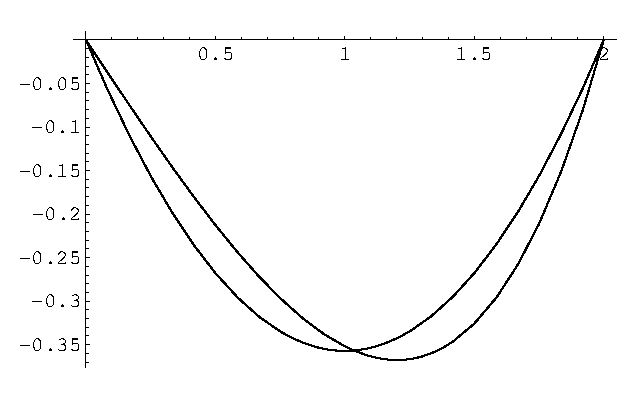
\includegraphics[width=0.4\textwidth]{cv/cv/p2_1t}
      \end{center}
      \caption{One term approximation and exact solution.}
      \label{p2_1t}
    \end{figure}

    The two term approximate solution is
    \[
    y(x) = x (2 - x) \left( - \frac{33}{161} - \frac{7}{46} x \right).
    \]
    This two term approximation and the exact solution are plotted in 
    Figure~\ref{p2_2t}.  The value of the functional is 
    \[
    J = - \frac{416}{805} \approx -0.51677.
    \]

    \begin{figure}[h!]
      \begin{center}
        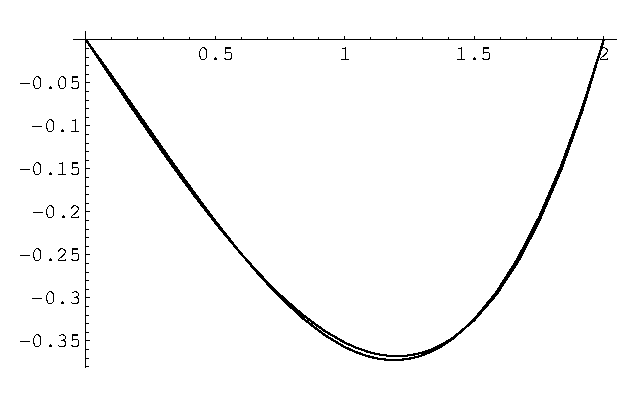
\includegraphics[width=0.4\textwidth]{cv/cv/p2_2t}
      \end{center}
      \caption{Two term approximation and exact solution.}
      \label{p2_2t}
    \end{figure}









    \textbf{Sine Series Approximation.}
    Consider an approximate solution of the form
    \[
    y(x) = a_1 \sin \left( \frac{\pi x}{2} \right)
    + a_2 \sin \left( \pi x \right) + \cdots +
    a_n \sin \left( n \frac{\pi x}{2} \right).
    \]
    The one term approximate solution is
    \[
    y(x) = - \frac{16}{ \pi (\pi^2 + 4) } \sin \left( \frac{\pi x}{2} \right).
    \]
    This one term approximation and the exact solution are plotted in 
    Figure~\ref{p2_1s}.  The value of the functional is 
    \[
    J = - \frac{64}{\pi^2 (\pi^2 + 4)} \approx -0.467537.
    \]

    \begin{figure}[h!]
      \begin{center}
        \includegraphics[width=0.4\textwidth]{cv/cv/p2_1s}
      \end{center}
      \caption{One term sine series approximation and exact solution.}
      \label{p2_1s}
    \end{figure}

    The two term approximate solution is
    \[
    y(x) = - \frac{16}{ \pi (\pi^2 + 4) } \sin \left( \frac{\pi x}{2} \right)
    + \frac{2}{\pi (\pi^2 + 1) } \sin (\pi x ).
    \]
    This two term approximation and the exact solution are plotted in 
    Figure~\ref{p2_2s}.  The value of the functional is 
    \[
    J = - \frac{4 (17\pi^2 + 20) }{ \pi^2 (\pi^4 + 5 \pi^2 + 4)} \approx -0.504823.
    \]

    \begin{figure}[h!]
      \begin{center}
        \includegraphics[width=0.4\textwidth]{cv/cv/p2_2s}
      \end{center}
      \caption{Two term sine series approximation and exact solution.}
      \label{p2_2s}
    \end{figure}
    %%
    %%
    %%
  \item
    \textbf{Exact Solution.}
    The Euler differential equation is
    \begin{gather*}
      \frac{\dd}{\dd x} F_{,y'} = F_{,y} \\
      \frac{\dd}{\dd x} [2 x y'] = - 2 \frac{x^2-1}{x} y - 2 x^2 \\
      y'' + \frac{1}{x} y' + \left( 1 - \frac{1}{x^2} \right) y = - x
      \intertext{The general solution is}
      y = c_1 J_1(x) + c_2 Y_1(x) - x
      \intertext{Applying the boundary conditions we obtain,}
      \boxed{
        y = \frac{ ( Y_1(2) - 2 Y_1(1) ) J_1(x) + ( 2 J_1(1) - J_1(2) ) Y_1(x) }
        { J_1(1) Y_1(2) - Y_1(1) J_1(2) } - x
        } 
    \end{gather*}
    The value of the integral for this extremal is
    \[
    \boxed{
      J \approx -0.310947
      }
    \]






    \textbf{Polynomial Approximation.}
    Consider an approximate solution of the form
    \[
    y(x) = (x-1) (2 - x) (a_0 + a_1 x + \cdots a_n x^n).
    \]
    The one term approximate solution is
    \[
    \boxed{
      y(x) = (x-1)(2-x) \frac{ 23 }{ 6 (40 \log 2 - 23 ) }
      }
    \]
    This one term approximation and the exact solution are plotted in 
    Figure~\ref{p3_1t}.  
    The one term approximation is a surprisingly close to the exact solution.
    The value of the functional is 
    \[
    \boxed{
      J = - \frac{ 529 }{ 360 (40 \log 2 - 23 ) } \approx -0.310935.
      }
    \]


    \begin{figure}[h!]
      \begin{center}
        \includegraphics[width=0.4\textwidth]{cv/cv/p3_1t}
      \end{center}
      \caption{One term polynomial approximation and exact solution.}
      \label{p3_1t}
    \end{figure}
  \end{enumerate}
\end{Solution}



%%Let $K(x)$ belong to $L_1(-\infty,\infty)$ and define the operator $T$ on
\begin{Solution}
  \begin{enumerate}
    %%
    %%
  \item
    The spectrum of $T$ is the set,
    \[
    \{ \lambda : (T - \lambda I)\ \mathrm{is not invertible}. \}
    \]
    \begin{gather*}
      (T - \lambda I) f = g \\
      \int_{-\infty}^\infty K(x - y) f(y) \,\dd y - \lambda f(x) = g \\
      \hat{K}(\omega) \hat{f}(\omega) - \lambda \hat{f}(\omega) = \hat{g}(\omega) \\
      \left( \hat{K}(\omega) - \lambda \right) \hat{f}(\omega) = \hat{g}(\omega) \\
    \end{gather*}
    We may not be able to solve for $\hat{f}(\omega)$, (and hence invert
    $T - \lambda I$), if $\lambda = \hat{K}(\omega)$.  Thus all values of 
    $\hat{K}(\omega)$ are in the spectrum.  If $\hat{K}(\omega)$ is everywhere
    nonzero we consider the case $\lambda = 0$.  We have the equation,
    \[
    \int_{-\infty}^\infty K(x - y) f(y) \,\dd y = 0 
    \]
    Since there are an infinite number of $L_2(-\infty,\infty)$ functions 
    which satisfy this, (those which are nonzero on a set of measure zero),
    we cannot invert the equation.  Thus $\lambda = 0$ is in the spectrum.
    The spectrum of $T$ is the range of $\hat{K}(\omega)$ plus zero.
    %%
    %%
  \item
    Let $\lambda$ be a nonzero eigenvalue with eigenfunction $\phi$.
    \begin{gather*}
      (T - \lambda I) \phi = 0, \quad \forall x \\
      \int_{-\infty}^\infty K(x - y) \phi(y) \,\dd y - \lambda \phi(x) = 0, \quad \forall x 
    \end{gather*}
    Since $K$ is continuous, $T \phi$ is continuous.  This implies that the 
    eigenfunction $\phi$ is continuous.  We take the Fourier transform of the
    above equation.
    \begin{gather*}
      \hat{K}(\omega) \hat{\phi}(\omega) - \lambda \hat{\phi}(\omega) = 0, \quad
      \forall \omega \\
      \left( \hat{K}(\omega) - \lambda \right) \hat{\phi}(\omega) = 0, \quad
      \forall \omega 
    \end{gather*}
    If $\phi(x)$ is absolutely integrable, then $\hat{\phi}(\omega)$ is continous.
    Since $\phi(x)$ is not identically zero, $\hat{\phi(\omega)}$ is not
    identically zero.  Continuity implies that $\hat{\phi(\omega)}$ is nonzero
    on some interval of positive length, $(a,b)$.  From the above equation 
    we see that $\hat{K}(\omega) = \lambda$ for $\omega \in (a,b)$.

    Now assume that $\hat{K}(\omega) = \lambda$ in some interval $(a,b)$.  
    Any function $\hat{\phi}(\omega)$ that is nonzero only for 
    $\omega \in (a,b)$ satisfies
    \[
    \left( \hat{K}(\omega) - \lambda \right) \hat{\phi}(\omega) = 0, \quad
    \forall \omega.
    \]
    By taking the inverse Fourier transform we obtain an eigenfunction 
    $\phi(x)$ of the eigenvalue $\lambda$.
    %%
    %%
  \item
    First we use the Fourier transform to find an explicit representation of
    $u = (T - \lambda I)^{-1} f$.
    \begin{gather*}
      u = (T - \lambda I)^{-1} f
      (T - \lambda I) u = f \\
      \int_{-\infty}^\infty K(x - y) u(y) \,\dd y - \lambda u = f \\
      2 \pi \hat{K} \hat{u} - \lambda \hat{u} = \hat{f} \\
      \hat{u} = \frac{ \hat{f} }{ 2 \pi \hat{K} - \lambda } \\
      \hat{u} = - \frac{1}{\lambda} \frac{ \hat{f} }{ 1 - 2 \pi \hat{K} / \lambda }\\
      \intertext{For $|\lambda| > |2 \pi \hat{K}|$ we can expand the denominator in 
        a geometric series.}
      \hat{u} = - \frac{1}{\lambda} \hat{f} 
      \sum_{n = 0}^\infty \left( \frac{ 2 \pi \hat{K} }{ \lambda } \right)^n \\
      \boxed{
        u = - \frac{1}{\lambda} \sum_{n = 0}^\infty \frac{1}{\lambda^n} 
        \int_{-\infty}^\infty K_n(x - y) f(y) \,\dd y
        }
    \end{gather*}
    Here $K_n$ is the $n^{\mathrm{th}}$ iterated kernel.  
    Now we form the Neumann series expansion.
    \begin{align*}
      u       &= \left( T - \lambda I \right)^{-1} f \\
      &=  - \frac{1}{\lambda} \left( I - \frac{1}{\lambda} T \right)^{-1} f\\
      &=  - \frac{1}{\lambda} \sum_{n = 0}^\infty \frac{1}{\lambda^n} T^n f \\
      &=  - \frac{1}{\lambda} \sum_{n = 0}^\infty \frac{1}{\lambda^n} T^n f \\
      &=  - \frac{1}{\lambda} \sum_{n = 0}^\infty \frac{1}{\lambda^n} 
      \int_{-\infty}^\infty K_n(x - y) f(y) \,\dd y
    \end{align*}
    The Neumann series is the same as the series we derived with the 
    Fourier transform.
  \end{enumerate}
\end{Solution}



%%Let $U$ be the space of twice continuously differentiable functions $f$ on
\begin{Solution}
  We seek a transformation $T$ such that
  \[
  (L - \lambda I) T f = f.
  \]
  We denote $u = T f$ to obtain a boundary value problem,
  \[
  u'' - \lambda u = f, \qquad u(-1) = u(1) = 0.
  \]
  This problem has a unique solution if and only if the homogeneous 
  adjoint problem has only the trivial solution.
  \[
  u'' - \lambda u = 0, \qquad u(-1) = u(1) = 0.
  \]
  This homogeneous problem has the eigenvalues and eigenfunctions,
  \[
  \lambda_n = - \left( \frac{n \pi}{2} \right)^2, \quad
  u_n = \sin\left( \frac{n \pi}{2} (x+1) \right), \quad
  n \in \mathbb{N}.
  \]
  The inhomogeneous problem has the unique solution 
  \[
  u(x) = \int_{-1}^1 G(x,\xi;\lambda) f(\xi) \,\dd \xi
  \]
  where
  \[
  G(x,\xi;\lambda) = 
  \begin{cases}
    - \frac{ \sin \left( \sqrt{-\lambda} (x_< +1) \right)
      \sin \left( \sqrt{-\lambda} (1-x_>) \right) }
    { \sqrt{-\lambda} \sin \left( 2 \sqrt{-\lambda} \right) },
    &\lambda < 0, \\
    - \frac{1}{2} (x_< + 1) (1 - x_>), &\lambda = 0, \\
    - \frac{ \sinh \left( \sqrt{\lambda} (x_< +1) \right)
      \sinh \left( \sqrt{\lambda} (1-x_>) \right) }
    { \sqrt{\lambda} \sinh \left( 2 \sqrt{\lambda} \right) },
    &\lambda > 0,
  \end{cases}
  \]
  for $\lambda \neq - (n \pi / 2)^2$, $n \in \mathbb{N}$.  We set
  \[
  T f = \int_{-1}^1 G(x,\xi;\lambda) f(\xi) \,\dd \xi
  \]
  and note that since the kernel is continuous this is a bounded linear
  transformation.  If $f \in W$, then
  \begin{align*}
    (L - \lambda I) T f 
    &= (L - \lambda I) \int_{-1}^1 G(x,\xi;\lambda) f(\xi) \,\dd \xi \\
    &= \int_{-1}^1 (L - \lambda I)[G(x,\xi;\lambda)] f(\xi) \,\dd \xi \\
    &= \int_{-1}^1 \delta(x - \xi) f(\xi) \,\dd \xi \\
    &= f(x).
  \end{align*}
  If $f \in U$ then
  \begin{align*}
    T (L - \lambda I) f
    &= \int_{-1}^1 G(x,\xi;\lambda) \big( f''(\xi) - \lambda f(\xi) \big)
    \,\dd \xi \\
    &= \left[ G(x,\xi;\lambda) f'(\xi) \right]_{-1}^1
    - \int_{-1}^1 G'(x,\xi;\lambda) f'(\xi) \,\dd \xi 
    - \lambda \int_{-1}^1 G(x,\xi;\lambda) f(\xi) \,\dd \xi \\
    &= \left[ - G'(x,\xi;\lambda) f(\xi) \right]_{-1}^1
    + \int_{-1}^1 G''(x,\xi;\lambda) f(\xi) \,\dd \xi 
    - \lambda \int_{-1}^1 G(x,\xi;\lambda) f(\xi) \,\dd \xi \\
    &= \int_{-1}^1 \big( G''(x,\xi;\lambda) - \lambda G(x,\xi;\lambda) 
    \big) f(\xi) \,\dd \xi \\
    &= \int_{-1}^1 \delta(x - \xi) f(\xi) \,\dd \xi \\
    &= f(x).
  \end{align*}
  $L$ has the point spectrum $\lambda_n = - (n \pi / 2)^2$, $n \in \mathbb{N}$.
\end{Solution}



%%\phi(x) = x + \lambda \int_0^1 \left( x^2 y - y^2 \right) \phi(y) \,\dd y \\
\begin{Solution}
  \begin{enumerate}
    %%
    %%
    %%
  \item
    We see that the solution is of the form $\phi(x) = a + x + b x^2$ for some 
    constants $a$ and $b$.  We substitute this into the integral equation.
    \begin{gather*}
      \phi(x) = x + \lambda \int_0^1 \left( x^2 y - y^2 \right) \phi(y) \,\dd y \\
      a + x + b x^2 = x + \lambda \int_0^1 \left( x^2 y - y^2 \right) 
      (a + x + b x^2)\,\dd y \\
      a + b x^2 = \frac{\lambda}{60} \left( - (15 + 20 a + 12 b) + 
        (20 + 30 a + 15 b) x^2 \right)
    \end{gather*}
    By equating the coefficients of $x^0$ and $x^2$ we solve for $a$ and $b$.
    \[
    a = - \frac{ \lambda (\lambda + 60) }{ 4 (\lambda^2 + 5 \lambda + 60 ) }, 
    \qquad
    b = - \frac{ 5 \lambda (\lambda - 60) }{ 6 (\lambda^2 + 5 \lambda + 60 ) } 
    \]
    Thus the solution of the integral equation is
    \[
    \boxed{
      \phi(x) = x - \frac{ \lambda }{ \lambda^2 + 5 \lambda + 60 }
      \left( \frac{ 5 ( \lambda - 24 ) }{ 6 } x^2 + \frac{ \lambda + 60 }{4}
      \right).
      }
    \]
    %%
    %%
    %%
  \item
    For $x < 1$ the integral equation reduces to
    \[
    \boxed{
      \phi(x) = x.
      }
    \]
    For $x \geq 1$ the integral equation becomes,
    \[
    \phi(x) = x + \lambda \int_0^1 \sin(x y) \phi(y) \,\dd y.
    \]
    We could solve this problem by writing down the Neumann series.  
    Instead we will use an eigenfunction expansion.
    Let $\{ \lambda_n \}$ and $\{ \phi_n \}$ be the eigenvalues and orthonormal 
    eigenfunctions of 
    \[
    \phi(x) = \lambda \int_0^1 \sin(x y) \phi(y) \,\dd y.
    \]
    We expand $\phi(x)$ and $x$ in terms of the eigenfunctions.
    \begin{align*}
      \phi(x) &= \sum_{n = 1}^\infty a_n \phi_n(x) \\
      x &= \sum_{n = 1}^\infty b_n \phi_n(x), \qquad b_n = \langle x, \phi_n(x) \rangle \\
    \end{align*}
    We determine the coefficients $a_n$ by substituting the series expansions
    into the Fredholm equation and equating coefficients of the eigenfunctions.
    \begin{gather*}
      \phi(x) = x + \lambda \int_0^1 \sin(x y) \phi(y) \,\dd y \\
      \sum_{n = 1}^\infty a_n \phi_n(x) = \sum_{n = 1}^\infty b_n \phi_n(x) 
      + \lambda \int_0^1 \sin(x y) \sum_{n = 1}^\infty a_n \phi_n(y) \,\dd y \\
      \sum_{n = 1}^\infty a_n \phi_n(x) = \sum_{n = 1}^\infty b_n \phi_n(x) 
      + \lambda \sum_{n = 1}^\infty a_n \frac{1}{\lambda_n} \phi_n(x) \\
      a_n \left( 1 - \frac{\lambda}{\lambda_n} \right) = b_n
    \end{gather*}
    If $\lambda$ is not an eigenvalue then we can solve for the $a_n$ to 
    obtain the unique solution.
    \[
    a_n = \frac{ b_n }{ 1 - \lambda / \lambda_n }
    = \frac{ \lambda_n b_n }{ \lambda_n - \lambda}
    = b_n + \frac{ \lambda b_n }{ \lambda_n - \lambda}
    \]
    \[
    \boxed{
      \phi(x) = x + \sum_{n = 1}^\infty \frac{ \lambda b_n }{ \lambda_n - \lambda } \phi_n(x),
      \quad \mathrm{for}\ x \geq 1.
      }
    \]
    If $\lambda = \lambda_m$, and $\langle x, \phi_m \rangle = 0$ then there is 
    the one parameter family of solutions,
    \[
    \boxed{
      \phi(x) = x + c \phi_m(x) + \sum_{\substack{n = 1 \\ n \neq m}}^\infty
      \frac{ \lambda b_n }{ \lambda_n - \lambda } \phi_n(x),
      \quad \mathrm{for}\ x \geq 1.
      }
    \]
    If $\lambda = \lambda_m$, and $\langle x, \phi_m \rangle \neq 0$ then there is 
    no solution.
  \end{enumerate}
\end{Solution}



%%Suppose that $K = L_1 L_2$, where $L_1 L_2 - L_2 L_1 = I$.  Show that if $x$
\begin{Solution}
  \begin{enumerate}
    %%
  \item
    \[
    K x = L_1 L_2 x = \lambda x
    \]
    \begin{align*}
      L_1 L_2 ( L_1 x )
      &= L_1 ( L_1 l_2 - I ) x \\
      &= L_1 ( \lambda x - x ) \\
      &= (\lambda - 1) (L_1 x)
    \end{align*}
    \begin{align*}
      L_1 L_2 ( L_2 x )
      &= ( L_2 L_1 + I ) L_2 x \\
      &= L_2 \lambda x + L_2 x \\
      &= (\lambda + 1) (L_2 x)
    \end{align*}
    %%
  \item
    \begin{align*}
      L_1 L_2 - L_2 L_1 
      &= \left( \frac{\dd}{\dd t} + \frac{t}{2} \right)
      \left( - \frac{\dd}{\dd t} + \frac{t}{2} \right)
      -  \left( - \frac{\dd}{\dd t} + \frac{t}{2} \right)
      \left( \frac{\dd}{\dd t} + \frac{t}{2} \right) \\
      &= - \frac{\dd}{\dd t} + \frac{t}{2} \frac{\dd}{\dd t} + \frac{1}{2} I 
      - \frac{t}{2} \frac{\dd}{\dd t} + \frac{t^2}{4} I
      - \left( - \frac{\dd}{\dd t} - \frac{t}{2} \frac{\dd}{\dd t} - \frac{1}{2} I 
        + \frac{t}{2} \frac{\dd}{\dd t} + \frac{t^2}{4} I \right) \\
      &= I
    \end{align*}
    \[
    L_1 L_2 = - \frac{\dd}{\dd t} + \frac{1}{2} I + \frac{t^2}{4} I
    = K + \frac{1}{2} I
    \]
    We note that $\e^{-t^2 / 4}$ is an eigenfunction corresponding to 
    the eigenvalue $\lambda = 1/2$.   Since $L_1 \e^{-t^2 / 4} = 0$ the result
    of this problem does not produce any negative eigenvalues.  However,
    $L_2^n \e^{-t^2 / 4}$ is the product of $\e^{-t^2 / 4}$ and a  polynomial 
    of degree $n$ in $t$.  Since this function is square integrable it is 
    and eigenfunction.  Thus we have the eigenvalues and eigenfunctions,
    \[
    \boxed{
      \lambda_n = n - \frac{1}{2}, \qquad
      \phi_n = \left( \frac{t}{2} - \frac{\dd}{\dd t} \right)^{n-1} \e^{-t^2 / 4}, \qquad
      \mathrm{for}\ n \in \mathbb{N}.
      }
    \]
  \end{enumerate}
\end{Solution}



%%Prove that if the value of $\lambda = \lambda_1$ is in the residual spectrum
\begin{Solution}
  Since $\lambda_1$ is in the residual spectrum of $T$, there exists a nonzero
  $y$ such that
  \[
  \langle (T - \lambda_1 I) x, y \rangle = 0
  \]
  for all $x$.  Now we apply the definition of the adjoint.
  \begin{gather*}
    \langle x, (T - \lambda_1 I)^* y \rangle = 0, \quad \forall x \\
    \langle x, (T^* - \overline{\lambda_1} I) y \rangle = 0, \quad \forall x \\
    (T^* - \overline{\lambda_1} I) y = 0
  \end{gather*}
  $y$ is an eigenfunction of $T^*$ corresponding to the eigenvalue 
  $\overline{\lambda_1}$.
\end{Solution}



%%u''(t) + \int_0^1 \sin(k(s-t)) u(s) \,\dd s = f(t), \quad
\begin{Solution}
  \begin{enumerate}
    %%
    %%
  \item
    \begin{gather*}
      u''(t) + \int_0^1 \sin(k(s-t)) u(s) \,\dd s = f(t), \quad u(0) = u'(0) = 0 \\
      u''(t) + \cos(k t) \int_0^1 \sin(k s) u(s) \,\dd s 
      - \sin(k t) \int_0^1 \cos(k s) u(s) \,\dd s = f(t) \\
      u''(t) + c_1 \cos(k t) - c_2 \sin(k t) = f(t) \\
      u''(t) = f(t) - c_1 \cos(k t) + c_2 \sin(k t) 
    \end{gather*}
    The solution of 
    \[
    u''(t) = g(t), \quad u(0) = u'(0) = 0
    \]
    using Green functions is
    \[
    u(t) = \int_0^t (t - \tau) g( \tau ) \,\dd \tau.
    \]
    Thus the solution of our problem has the form,
    \begin{gather*}
      u(t) = \int_0^t (t-\tau) f(\tau) \,\dd \tau 
      - c_1 \int_0^t (t - \tau) \cos(k \tau) \,\dd \tau
      + c_2 \int_0^t (t - \tau) \sin(k \tau) \,\dd \tau \\
      \boxed{
        u(t) = \int_0^t (t-\tau) f(\tau) \,\dd \tau 
        - c_1 \frac{1 - \cos(k t)}{k^2}
        + c_2 \frac{k t - \sin(k t)}{ k^2 }
        }
    \end{gather*}
    We could determine the constants by multiplying in turn by $\cos(k t)$ 
    and $\sin(k t)$ and integrating from $0$ to $1$.  This would yields a set 
    of two linear equations for $c_1$ and $c_2$.
    %%
    %%
  \item
    \[
    u(x) = \lambda \int_0^\pi \sum_{n = 1}^\infty \frac{ \sin n x \sin n s }{ n } u(s) \,\dd s
    \]
    We expand $u(x)$ in a sine series.
    \begin{gather*}
      \sum_{n = 1}^\infty a_n \sin n x 
      = \lambda \int_0^\pi \left( \sum_{n = 1}^\infty \frac{ \sin n x \sin n s }{ n } 
      \right) \left( \sum_{m = 1}^\infty a_m \sin m s \right) \,\dd s \\
      \sum_{n = 1}^\infty a_n \sin n x 
      = \lambda \sum_{n = 1}^\infty \frac{ \sin n x }{ n } \sum_{m = 1}^\infty \int_0^\pi 
      a_m \sin n s \sin m s \,\dd s \\
      \sum_{n = 1}^\infty a_n \sin n x 
      = \lambda \sum_{n = 1}^\infty \frac{ \sin n x }{ n } \sum_{m = 1}^\infty \frac{\pi}{2}
      a_m \delta_{m n} \\
      \sum_{n = 1}^\infty a_n \sin n x 
      = \frac{\pi}{2} \lambda \sum_{n = 1}^\infty a_n \frac{ \sin n x }{ n } 
    \end{gather*}
    The eigenvalues and eigenfunctions are
    \[
    \boxed{
      \lambda_n = \frac{ 2 n }{ \pi }, \qquad
      u_n = \sin n x, \qquad
      n \in \mathbb{N}.
      }
    \]
    %%
    %%
  \item
    \[
    \phi(\theta) = \lambda \int_0^{2 \pi} \frac{1}{2 \pi} \frac{ 1 - r^2 }
    { 1 - 2 r \cos (\theta - t) + r^2 } \phi(t) \,\dd t, \quad
    |r| < 1
    \]
    We use Poisson's formula.
    \[
    \phi(\theta) = \lambda u(r,\theta),
    \]
    where $u(r,\theta)$ is harmonic in the unit disk and satisfies,
    $u(1, \theta) = \phi(\theta)$.  For a solution we need $\lambda = 1$
    and that $u(r,\theta)$ is independent of $r$.  In this case $u(\theta)$
    satisfies
    \[
    u''(\theta) = 0, \quad u(\theta) = \phi(\theta).
    \]
    The solution is $\phi(\theta) = c_1 + c_2 \theta$.
    There is only one eigenvalue and corresponding eigenfunction,
    \[
    \boxed{
      \lambda = 1, \qquad \phi = c_1 + c_2 \theta.
      }
    \]
    %%
    %%
  \item
    \[
    \phi(x) = \lambda \int_{-\pi}^\pi \cos^n (x - \xi) \phi(\xi) \,\dd \xi
    \]
    We expand the kernel in a Fourier series.
    We could find the expansion by integrating to find the Fourier
    coefficients, but it is easier to expand $\cos^n(x)$ directly.
    \begin{align*}
      \cos^n(x)
      &= \left[ \frac{1}{2} (\e^{\imath x} + \e^{-\imath x}) \right]^n \\
      &= \frac{1}{2^n} \left[ \binom{n}{0} \e^{\imath n x} +
        \binom{n}{1} \e^{\imath (n-2)x} + \cdots +
        \binom{n}{n-1} \e^{-\imath (n-2)x} + \binom{n}{n} \e^{-\imath n x} \right]
    \end{align*}
    If $n$ is odd,
    \begin{align*}
      \cos^n(x)
      &= \frac{1}{2^n} \Bigg[ \binom{n}{0} (\e^{\imath n x} + \e^{-\imath n x})
      + \binom{n}{1} (\e^{\imath (n-2)x} + \e^{-\imath (n-2)x}) + \cdots \\
      &\qquad\qquad + \binom{n}{(n-1)/2}(\e^{\imath x} + \e^{-\imath x}) \Bigg] \\
      &= \frac{1}{2^n} \left[ \binom{n}{0} 2 \cos(n x)
        + \binom{n}{1} 2 \cos((n-2)x) + \cdots +
        \binom{n}{(n-1)/2}2\cos(x) \right] \\
      &= \frac{1}{2^{n-1}} \sum_{m=0}^{(n-1)/2} \binom{n}{m}
      \cos((n-2m)x) \\
      &= \frac{1}{2^{n-1}} \sum_{\substack{k = 1 \\ \mathrm{odd}\ k}}^n
      \binom{ n }{ (n-k)/2 } \cos(k x).
    \end{align*}
    If $n$ is even,
    \begin{align*}
      \cos^n(x)
      &= \frac{1}{2^n} \Bigg[ \binom{n}{0}(\e^{\imath n x}+\e^{-\imath n x})
      + \binom{n}{1} (\e^{\imath (n-2)x}+\e^{-\imath (n-2)x}) + \cdots \\
      &\qquad\qquad + \binom{n}{n/2-1} (\e^{i2x}+\e^{-i2x}) 
      + \binom{n}{n/2}\Bigg] \\
      &= \frac{1}{2^n} \left[ \binom{n}{0}2\cos(n x)
        + \binom{n}{1} 2\cos((n-2)x) + \cdots +
        \binom{n}{n/2-1} 2\cos(2x) + \binom{n}{n/2}\right] \\
      &= \frac{1}{2^n} \binom{n}{n/2} + \frac{1}{2^{n-1}} \sum_{m=0}^{(n-2)/2}
      \binom{n}{m} \cos((n-2m)x) \\
      &= \frac{1}{2^n} \binom{n}{n/2}
      + \frac{1}{2^{n-1}} \sum_{\substack{k = 2 \\ \mathrm{even}\ k}}^n
      \binom{ n }{ (n-k)/2 } \cos(k x).
    \end{align*}
    We will denote,
    \[
    \cos^n (x - \xi) = \frac{a_0}{2} \sum_{k = 1}^n a_k \cos(k (x - \xi) ),
    \]
    where
    \[
    a_k = \frac{ 1 + (-1)^{n-k} }{2} \frac{1}{2^{n-1}} \binom{ n }{ (n-k)/2 }.
    \]
    We substitute this into the integral equation.
    \begin{gather*}
      \phi(x) = \lambda \int_{-\pi}^\pi  
      \left( \frac{a_0}{2} \sum_{k = 1}^n a_k \cos(k (x - \xi) ) \right)
      \phi(\xi) \,\dd \xi \\
      \phi(x) = \lambda \frac{a_0}{2} \int_{-\pi}^\pi \phi(\xi) \,\dd \xi + 
      \lambda \sum_{k = 1}^n a_k \left( 
        \cos(k x) \int_{-\pi}^\pi \cos(k \xi) \phi(\xi) \,\dd \xi
        + \sin(k x) \int_{-\pi}^\pi \sin(k \xi) \phi(\xi) \,\dd \xi \right)
    \end{gather*}
    For even $n$, substituting $\phi(x) = 1$ yields $\lambda = \frac{1}{\pi a_0}$.
    For $n$ and $m$ both even or odd, substituting $\phi(x) = \cos(m x)$ or 
    $\phi(x) = \sin(m x)$ yields $\lambda = \frac{1}{\pi a_m}$.  
    For even $n$ we have the eigenvalues and eigenvectors,
    \begin{gather*}
      \lambda_0 = \frac{1}{\pi a_0}, \qquad \phi_0 = 1, \\
      \lambda_m = \frac{1}{\pi a_{2m}}, \qquad \phi^{(1)}_m = \cos(2 m x),
      \quad \phi^{(2)}_m = \sin(2 m x), \qquad m = 1, 2, \ldots, n/2.
    \end{gather*}
    For odd $n$ we have the eigenvalues and eigenvectors,
    \[
    \lambda_m = \frac{1}{\pi a_{2m-1}}, \qquad \phi^{(1)}_m = \cos((2 m - 1) x),
    \quad \phi^{(2)}_m = \sin((2 m - 1) x), \qquad m = 1, 2, \ldots, (n+1)/2.
    \]
  \end{enumerate}
\end{Solution}



%%Let $K(x,s) = 2 \pi^2 - 6 \pi |x-s| + 3 (x-s)^2$.
\begin{Solution}
  \begin{enumerate}
    %%
    %%
  \item
    First we shift the range of integration to rewrite the kernel.
    \begin{gather*}
      \phi(x) = \lambda \int_0^{2 \pi} \left( 2 \pi^2 - 6 \pi |x-s| + 3 (x-s)^2 
      \right) \phi(s) \,\dd s \\
      \phi(x) = \lambda \int_{-x}^{-x + 2 \pi} \left( 2 \pi^2 - 6 \pi |y| + 3 y^2 
      \right) \phi(x+y) \,\dd y 
    \end{gather*}
    We expand the kernel in a Fourier series.
    \[
    K(y) = 2 \pi^2 - 6 \pi |y| + 3 y^2 = \sum_{n = -\infty}^\infty c_n \e^{\imath n y}
    \]
    \[
    c_n = \frac{1}{2 \pi} \int_{-x}^{-x+2\pi} K(y) \e^{-\imath n y} \,\dd y = 
    \begin{cases}
      \frac{6}{n^2}, &n \neq 0, \\
      0,      &n = 0
    \end{cases}
    \]
    \[
    K(y) = \sum_{\substack{n = -\infty \\ n \neq 0}}^\infty \frac{6}{n^2} 
    \e^{\imath n y} 
    = \sum_{n = 1}^\infty \frac{12}{n^2} \cos(n y) 
    \]
    \[
    K(x,s) = \sum_{n = 1}^\infty \frac{12}{n^2} \cos(n (x-s)) 
    = \sum_{n = 1}^\infty \frac{12}{n^2} \big( \cos(n x) \cos(n x) 
    + \sin(n x) \sin(n s) \big)
    \]
    Now we substitute the Fourier series expression for the kernel into the
    eigenvalue problem.
    \[
    \phi(x) = 12 \lambda \int_0^{2\pi} \left( \sum_{n = 1}^\infty \frac{1}{n^2} \big(
      \cos(n x) \cos(n s) + \sin(n x) \sin(n s) \big) \right) \phi(s) \,\dd s
    \]
    From this we obtain the eigenvalues and eigenfunctions,
    \[
    \boxed{
      \lambda_n = \frac{n^2}{12 \pi}, 
      \quad \phi_n^{(1)} = \frac{1}{\sqrt{\pi}} \cos(n x), 
      \quad \phi_n^{(2)} = \frac{1}{\sqrt{\pi}} \sin(n x), 
      \quad n \in \mathbb{N}.
      }
    \]
    %%
    %%
  \item
    The set of eigenfunctions do not form a complete set.  Only those functions
    with a vanishing integral on $[0,2\pi]$ can be represented.  We consider the
    equation
    \begin{gather*}
      \int_0^{2\pi} K(x,s) \phi(s) \,\dd s = 0 \\
      \int_0^{2\pi} \left( \sum_{n = 1}^\infty \frac{12}{n^2} \big(
        \cos(n x) \cos(n s) + \sin(n x) \sin(n s) \big) \right) \phi(s) \,\dd s
      = 0
    \end{gather*}
    This has the solutions $\phi = \mathrm{const}$.  The set of eigenfunctions
    \[
    \boxed{
      \phi_0 = \frac{1}{\sqrt{2\pi}},
      \quad \phi_n^{(1)} = \frac{1}{\sqrt{\pi}} \cos(n x), 
      \quad \phi_n^{(2)} = \frac{1}{\sqrt{\pi}} \sin(n x), 
      \quad n \in \mathbb{N},
      }
    \]
    is a complete set.
    We can also write the eigenfunctions as
    \[
    \boxed{
      \phi_n = \frac{1}{\sqrt{2 \pi}} \e^{\imath n x}, \quad n \in \mathbb{Z}.
      }
    \]
    %%
    %%
  \item
    We consider the problem 
    \[
    u - \lambda T u = f.
    \]
    For $\lambda \neq \lambda$, ($\lambda$ not an eigenvalue), we can obtain
    a unique solution for $u$.  
    \[
    u(x) = f(x) + \int_0^{2\pi} \Gamma(x,s,\lambda) f(s) \,\dd s
    \]
    Since $K(x,s)$ is self-adjoint and $L_2(0,2\pi)$, we have
    \begin{align*}
      \Gamma(x,s,\lambda)
      &= \lambda \sum_{\substack{n = -\infty \\ n \neq 0}}^\infty
      \frac{ \phi_n(x) \overline{\phi_n(s)} }{ \lambda_n - \lambda } \\
      &= \lambda \sum_{\substack{n = -\infty \\ n \neq 0}}^\infty
      \frac{ \frac{1}{2\pi} \e^{\imath n x} \e^{-\imath n s} }
      { \frac{n^2}{12 \pi} - \lambda } \\
      &= 6 \lambda \sum_{\substack{n = -\infty \\ n \neq 0}}^\infty
      \frac{ \e^{\imath n (x-s)} }{ n^2 - 12 \pi \lambda } 
    \end{align*}
    \[
    \boxed{
      \Gamma(x,s,\lambda)
      = 12 \lambda \sum_{n = 1}^\infty \frac{ \cos(n(x-s)) }{ n^2 - 12 \pi \lambda }
      }
    \]
  \end{enumerate}
\end{Solution}



%%Let $K(x,s)$ be a bounded self-adjoint kernel on the finite interval $(a,b)$,
\begin{Solution}
  First assume that $\lambda$ is an eigenvalue of $T$, $T \phi = \lambda \phi$.
  \begin{align*}
    p(T) \phi
    &= \sum_{k = 0}^n a_n T^n \phi \\
    &= \sum_{k = 0}^n a_n \lambda^n \phi \\
    &= p(\lambda) \phi
  \end{align*}
  $p(\lambda)$ is an eigenvalue of $p(T)$.

  Now assume that $\mu$ is an eigenvalues of $p(T)$, $p(T) \phi = \mu \phi$.
  We assume that $T$ has a complete, orthonormal set of eigenfunctions, 
  $\{ \phi_n \}$ corresponding to the set of eigenvalues $\{\lambda_n\}$.  
  We expand $\phi$ in these eigenfunctions.
  \begin{gather*}
    p(T) \phi = \mu \phi \\
    p(T) \sum c_n \phi_n = \mu \sum c_n \phi_n \\
    \sum c_n p(\lambda_n) \phi_n = \sum c_n \mu \phi_n \\
    p(\lambda_n) = \mu, \quad \forall n\ \mathrm{such that}\ c_n \neq 0
  \end{gather*}
  Thus all eigenvalues of $p(T)$ are of the form $p(\lambda)$ with $\lambda$
  an eigenvalue of $T$.
\end{Solution}



%%\phi(x) = f(x) + \lambda \int_0^\infty \cos(2 x s) \phi(s) \,\dd s
\begin{Solution}
  The Fourier cosine transform is defined,
  \begin{align*}
    \hat{f}(\omega) &= \frac{1}{\pi} \int_0^\infty f(x) \cos(\omega x) \,\dd x, \\
    f(x) &= 2 \int_0^\infty \hat{f}(\omega) \cos(\omega x) \,\dd \omega. 
  \end{align*}
  We can write the integral equation in terms of the Fourier cosine transform.
  \[
  \phi(x) = f(x) + \lambda \int_0^\infty \cos(2 x s) \phi(s) \,\dd s
  \]
  \begin{equation}
    \label{phi=f+lpp}
    \phi(x) = f(x) + \lambda \pi \hat{\phi}(2 x)
  \end{equation}
  We multiply the integral equation by $\frac{1}{\pi} \cos(2 x s)$ and integrate.
  \begin{gather*}
    \frac{1}{\pi} \int_0^\infty \cos(2 x s) \phi(x)\,\dd x 
    = \frac{1}{\pi} \int_0^\infty \cos(2 x s) f(x)\,\dd x 
    + \lambda \int_0^\infty \cos(2 x s) \hat{\phi}(2 x)\,\dd x \\
    \hat{\phi}(2 s) = \hat{f}(2 s)  
    + \frac{ \lambda }{ 2 } \int_0^\infty \cos(x s) \hat{\phi}(x)\,\dd x \\
    \hat{\phi}(2 s) = \hat{f}(2 s) + \frac{ \lambda }{ 4 } \phi(s) \\
  \end{gather*}
  \begin{equation}
    \label{fct_phi=f+lpp}
    \phi(x) = - \frac{4}{\lambda} \hat{f}(2 x) + \frac{4}{\lambda} \hat{\phi}(2 x)
  \end{equation}
  We eliminate $\hat{\phi}$ between (\ref{phi=f+lpp}) and (\ref{fct_phi=f+lpp}).
  \begin{gather*}
    \left( 1 - \frac{\pi \lambda^2}{4} \right) \phi(x) 
    = f(x) + \lambda \pi \hat{f}(2 x) \\
    \boxed{
      \phi(x) = \frac{ f(x) + \lambda \int_0^\infty f(s) \cos(2 x s) \,\dd s }
      { 1 - \pi \lambda^2 / 4 }
      }
  \end{gather*}
\end{Solution}



%%L u = 0 \mathrm{ in } D, \quad u = f \mathrm{ on } C,
\begin{Solution}
  \begin{align*}
    \int_D v L u \,\dd x \,\dd y
    &= \int_D v ( u_{x x} + u_{y y} + a u_x + b u_y + c u ) \,\dd x \,\dd y \\
    &= \int_D ( v \nabla^2 u + a v u_x + b v u_y + c u v )\,\dd x\,\dd y \\
    &= \int_D ( u \nabla^2 v + a v u_x + b v u_y + c u v )\,\dd x\,\dd y 
    + \int_C ( v \nabla u - u \nabla v ) \cdot n \,\dd s \\
    &= \int_D ( u \nabla^2 v - a u v_x - b u v_y - u v a_x - u v b_y
    + c u v )\,\dd x\,\dd y 
    + \int_C \left( a u v \frac{\partial x}{\partial n} + b u v \frac{\partial y}{\partial n} \right) 
    \,\dd s
    + \int_C \left( v \frac{\partial u}{\partial n} - u \frac{\partial v}{\partial n} \right) \,\dd s 
  \end{align*}
  Thus we see that
  \[
  \int_D ( v L u - u L^* v)\,\dd x \,\dd y = \int_C H(u,v)\,\dd s,
  \]
  where
  \[
  L^* v = v_{x x} + v_{y y} - a v_x - b v_y + (c - a_x - b_y) v
  \]
  and
  \[
  H(u,v) = \left( v \frac{\partial u}{\partial n} - u \frac{\partial v}{\partial n} + a u v \frac{\partial x}{\partial n}
    + b u v \frac{\partial y}{\partial n} \right).
  \]




  Let $G$ be the harmonic Green function, which satisfies,
  \[
  \Delta G = \delta\ \mathrm{in}\ D, \quad G = 0\ \mathrm{on}\ C.
  \]
  Let $u$ satisfy $L u = 0$.
  \begin{gather*}
    \int_D ( G L u - u L^* G)\,\dd x \,\dd y = \int_C H(u,G)\,\dd s \\
    - \int_D u L^* G \,\dd x \,\dd y = \int_C H(u,G)\,\dd s \\
    - \int_D u \Delta G \,\dd x \,\dd y - \int_D u (L^* - \Delta) G \,\dd x \,\dd y 
    = \int_C H(u,G)\,\dd s \\
    - \int_D u \delta(x-\xi) \delta(y-\eta) \,\dd x \,\dd y 
    - \int_D u (L^* - \Delta) G \,\dd x \,\dd y = \int_C H(u,G)\,\dd s \\
    - u(\xi, \eta) - \int_D u (L^* - \Delta) G \,\dd x \,\dd y = \int_C H(u,G)\,\dd s 
  \end{gather*}

  We expand the operators to obtain the first form.
  \begin{gather*}
    u + \int_D u ( -a G_x - b G_y + (c - a_x - b_y) G ) \,\dd x \,\dd y 
    = - \int_C \left( G \frac{\partial u}{\partial n} - u \frac{\partial G}{\partial n} 
      + a u G \frac{\partial x}{\partial n} + b u G \frac{\partial y}{\partial n} \right) \,\dd s \\
    u + \int_D ( (c - a_x - b_y) G - a G_x - b G_y ) u \,\dd x \,\dd y 
    = \int_C u \frac{\partial G}{\partial n} \,\dd s \\
    u + \int_D ( (c - a_x - b_y) G - a G_x - b G_y ) u \,\dd x \,\dd y = U
  \end{gather*}
  Here $U$ is the harmonic function that satisfies $U = f$ on $C$.





  We use integration by parts to obtain the second form.
  \begin{gather*}
    u + \int_D ( c u G - a_x u G - b_y u G  - a u G_x - b u G_y ) \,\dd x \,\dd y = U\\
    u + \int_D ( c u G - a_x u G - b_y u G  + (a u)_x G + (b u)_y G ) \,\dd x \,\dd y 
    - \int_C \left(a u G \frac{\partial y}{\partial n} + b u G \frac{\partial x}{\partial n} \right)\,\dd s
    = U \\
    u + \int_D ( c u G - a_x u G - b_y u G  + a_x u G + a u_x G 
    + b_y u G + b u_y G ) \,\dd x \,\dd y = U \\
    \boxed{
      u + \int_D ( a u_x + b u_y + c u ) G \,\dd x \,\dd y = U 
      }
  \end{gather*}
\end{Solution}



%%Find the eigenvalues and eigenfunctions of the following kernels on 
\begin{Solution}
  \begin{enumerate}
    %%
    %%
  \item
    First we differentiate to obtain a differential equation.
    \begin{gather*}
      \phi(x)
      = \lambda \int_0^1 \min(x,s) \phi(s) \,\dd s 
      = \lambda \left( \int_0^x \e^s \phi(s) \,\dd s 
        + \int_x^1 \e^x \phi(s) \,\dd s \right) \\
      \phi'(x) 
      = \lambda \left( x \phi(x) + \int_x^1 \phi(s) \,\dd s - x \phi(x) \right)
      = \lambda \int_x^1 \phi(s) \,\dd s \\
      \phi''(x) = - \lambda \phi(x)
    \end{gather*}
    We note that that $\phi(x)$ satisfies the constraints,
    \begin{gather*}
      \phi(0) = \lambda \int_0^1 0 \cdot \phi(s) \,\dd s = 0, \\
      \phi'(1) = \lambda \int_1^1 \phi(s) \,\dd s = 0. 
    \end{gather*}
    Thus we have the problem,
    \[
    \phi'' + \lambda \phi = 0, \qquad
    \phi(0) = \phi'(1) = 0.
    \]
    The general solution of the differential equation is
    \[
    \phi(x) = 
    \begin{cases}
      a + b x &\mathrm{for}\ \lambda = 0 \\
      a \cos \left( \sqrt{\lambda} x \right) 
      + b \sin \left( \sqrt{\lambda} x \right) 
      &\mathrm{for}\ \lambda > 0 \\
      a \cosh \left( \sqrt{-\lambda} x \right) 
      + b \sinh \left( \sqrt{-\lambda} x \right) 
      &\mathrm{for}\ \lambda < 0
    \end{cases}
    \]
    We see that for $\lambda = 0$ and $\lambda < 0$ only the trivial solution
    satisfies the homogeneous boundary conditions.  For positive $\lambda$ the 
    left boundary condition demands that $a = 0$.  The right boundary condition is
    then
    \[
    b \sqrt{\lambda} \cos \left( \sqrt{\lambda} \right) = 0
    \]
    The eigenvalues and eigenfunctions are
    \[
    \boxed{
      \lambda_n = \left( \frac{ (2n-1) \pi }{ 2 } \right)^2, \quad
      \phi_n(x) = \sin \left( \frac{ (2n-1) \pi }{ 2 } x \right), \quad
      n \in \mathbb{N}
      }
    \]
    %%
    %%
  \item
    First we differentiate the integral equation.
    \begin{align*}
      \phi(x) &= \lambda \left( \int_0^x \e^s \phi(s) \,\dd s
        + \int_x^1 \e^x \phi(s) \,\dd s \right) \\
      \phi'(x) &= \lambda \left( \e^x \phi(x) + \e^x \int_x^1 \phi(s) \,\dd s
        - \e^x \phi(x) \right) \\
      &= \lambda \e^x \int_x^1 \phi(s) \,\dd s \\
      \phi''(x) &= \lambda \left( \e^x \int_x^1 \phi(s) \,\dd s - \e^x \phi(x) \right)
    \end{align*}
    $\phi(x)$ satisfies the differential equation
    \[
    \phi'' - \phi' + \lambda \e^x \phi = 0.
    \]
    We note the boundary conditions,
    \[
    \phi(0) - \phi'(0) = 0, \quad
    \phi'(1) = 0.
    \]
    In self-adjoint form, the problem is
    \[
    \left( \e^{-x} \phi' \right)' + \lambda \phi = 0, \quad 
    \phi(0) - \phi'(0) = 0, \quad
    \phi'(1) = 0.
    \]
    The Rayleigh quotient is
    \begin{align*}
      \lambda &=  \frac{ \left[ - \e^{-x} \phi \phi' \right]_0^1
        + \int_0^1 \e^{-x} (\phi')^2 \,\dd x }
      { \int_0^1 \phi^2 \,\dd x } \\
      &=  \frac{ \phi(0) \phi'(0)
        + \int_0^1 \e^{-x} (\phi')^2 \,\dd x }
      { \int_0^1 \phi^2 \,\dd x } \\
      &=  \frac{ (\phi(0))^2 + \int_0^1 \e^{-x} (\phi')^2 \,\dd x }
      { \int_0^1 \phi^2 \,\dd x } 
    \end{align*}
    Thus we see that there are only positive eigenvalues.
    The differential equation has the general solution
    \[
    \phi(x) = 
    \e^{x/2} \left( a J_1 \left( 2 \sqrt{\lambda} \e^{x/2} \right)
      + b Y_1 \left( 2 \sqrt{\lambda} \e^{x/2} \right) \right)
    \]
    We define the functions,
    \[
    u(x;\lambda) = 
    \e^{x/2} J_1 \left( 2 \sqrt{\lambda} \e^{x/2} \right), \quad
    v(x;\lambda) = 
    \e^{x/2} Y_1 \left( 2 \sqrt{\lambda} \e^{x/2} \right).
    \]
    We write the 
    solution to automatically satisfy the right boundary condition, 
    $\phi'(1) = 0$,
    \[
    \phi(x) = v'(1;\lambda) u(x;\lambda) - u'(1;\lambda) v(x;\lambda).
    \]
    We determine the eigenvalues from the left boundary condition, 
    $\phi(0) - \phi'(0) = 0$.  The first few are
    \begin{align*}
      \lambda_1 &\approx 0.678298 \\
      \lambda_2 &\approx 7.27931 \\
      \lambda_3 &\approx 24.9302 \\
      \lambda_4 &\approx 54.2593 \\
      \lambda_5 &\approx 95.3057 
    \end{align*}
    The eigenfunctions are,
    \[
    \phi_n(x) = v'(1;\lambda_n) u(x;\lambda_n) - u'(1;\lambda_n) v(x;\lambda_n).
    \]
  \end{enumerate}
\end{Solution}



%%\pv\int_{-\infty}^\infty \frac{ \sin(k x) \sin(l x) }{ x^2 - z^2 } \,\dd x
\begin{Solution}
  \begin{enumerate}
    %%-----------------------------------------------------------------------------
  \item
    First note that 
    \[
    \sin(k x) \sin(l x) = \sign(k l) \sin(a x) \sin(b x)
    \]
    where
    \[
    a = \max(|k|,|l|), \quad b = \min(|k|,|l|).
    \]
    Consider the analytic function,
    \[
    \frac{ \e^{\imath (a-b)x} - \e^{\imath (a+b)} }{2}
    = \sin(a x) \sin(b x) - \imath \cos(a x) \sin(b x).
    \]
    \begin{align*}
      \pv\int_{-\infty}^\infty \frac{ \sin(k x) \sin(l x) }{ x^2 - z^2 } \,\dd x
      &= \sign(k l) \pv\int_{-\infty}^\infty \frac{ \sin(a x) \sin(b x) }{ x^2 - z^2 } 
      \,\dd x \\
      &= \sign(k l) \frac{1}{2 z} \pv\int_{-\infty}^\infty 
      \left( \frac{ \sin(a x) \sin(b x) }{ x - z } 
        - \frac{ \sin(a x) \sin(b x) }{ x + z } \right) \,\dd x \\
      &= - \pi \sign(k l) \frac{1}{2 z} \left( - \cos(a z) \sin(b z)
        + \cos(-a z) \sin(-b z) \right) 
    \end{align*}
    \[
    \boxed{
      \pv\int_{-\infty}^\infty \frac{ \sin(k x) \sin(l x) }{ x^2 - z^2 } \,\dd x 
      = \sign(k l) \frac{\pi}{z} \cos(a z) \sin(b z)
      }
    \]
    %%-----------------------------------------------------------------------------
  \item
    Consider the analytic function,
    \[
    \frac{ \e^{\imath |p| x} - \e^{\imath |q| x} }{x}
    = \frac{ \cos(|p| x) - \cos(|q| x) + \imath ( \sin(|p| x) - \sin(|q| x)) }{x}.
    \]
    \begin{align*}
      \pv\int_{-\infty}^\infty \frac{ \cos(p x) - \cos(q x) }{x^2} \,\dd x
      &= \pv\int_{-\infty}^\infty \frac{ \cos(|p| x) - \cos(|q| x) }{x^2} \,\dd x \\
      &= -\pi \lim_{x \to 0} \frac{ \sin(|p| x) - \sin(|q| x) }{x} 
    \end{align*}
    \[
    \boxed{
      \pv\int_{-\infty}^\infty \frac{ \cos(p x) - \cos(q x) }{x^2} \,\dd x = \pi (|q| - |p|)
      }
    \]
    %%-----------------------------------------------------------------------------
  \item
    We use the analytic function,
    \[
    \frac{ \imath (x - \imath a)(x - \imath b) \e^{\imath x} }{ (x^2 + a^2)(x^2 + b^2) }
    = \frac{ - (x^2 - a b) \sin x + (a + b) x \cos x + 
      \imath ((x^2 - a b) \cos x + (a+b) x \sin x ) }{ (x^2+a^2)(x^2+b^2) }
    \]
    \begin{align*}
      \pv\int_{-\infty}^\infty \frac{ - (x^2 - a b) \sin x + (a + b) x \cos x }
      { x (x^2+a^2)(x^2+b^2) }
      &= - \pi \lim_{x \to 0} \frac{ (x^2 - a b) \cos x + (a+b) x \sin x }
      { (x^2+a^2)(x^2+b^2) } \\
      &= - \pi \frac{- a b}{a^2 b^2}
    \end{align*}
    \[
    \boxed{
      \pv\int_{-\infty}^\infty \frac{ - (x^2 - a b) \sin x + (a + b) x \cos x }
      { (x^2+a^2)(x^2+b^2) } = \frac{\pi}{a b}
      }
    \]
  \end{enumerate}
\end{Solution}



%%\pv\int_{-\infty}^\infty \frac{ (1-t^2)^{1/2} \log(1+t) }{ t-x } \,\dd t
\begin{Solution}
  We consider the function
  \[
  G(z) = \left( (1-z^2)^{1/2} + \imath z \right) \log(1+z).
  \]
  For $(1-z^2)^{1/2} = (1-z)^{1/2} (1+z)^{1/2}$ we choose the angles,
  \[
  -\pi < \arg(1-z) < \pi, \quad 0 < \arg(1+z) < 2\pi, 
  \]
  so that there is a branch cut on the interval $(-1,1)$.  With this choice
  of branch, $G(z)$ vanishes at infinity.  
  For the logarithm we choose the principal branch,
  \[
  -\pi < \arg(1+z) < \pi.
  \]

  For $t \in (-1,1)$,
  \begin{align*}
    G^+(t) &= \left( \sqrt{1-t^2} + \imath t \right) \log(1+t), \\
    G^-(t) &= \left( -\sqrt{1-t^2} + \imath t \right) \log(1+t), 
  \end{align*}
  \begin{align*}
    G^+(t) - G^-(t) &= 2 \sqrt{1-t^2} \log(1+t), \\
    \frac{1}{2} \left( G^+(t) + G^-(t) \right) &= \imath t \log(1+t).
  \end{align*}
  For $t \in (-\infty,-1)$,
  \begin{align*}
    G^+(t) &= \imath \left( \sqrt{1-t^2} + t \right) \left( \log(-t-1) + \imath \pi \right),\\
    G^-(t) &= \imath \left( -\sqrt{1-t^2} + t \right) \left( \log(-t-1) - \imath \pi \right), 
  \end{align*}
  \[
  G^+(t) - G^-(t) = - 2 \pi \left( \sqrt{t^2 - 1} + t \right).
  \]
  For $x \in (-1,1)$ we have
  \begin{align*}
    G(x)
    &= \frac{1}{2} \left( G^+(x) + G^-(x) \right) \\
    &= \imath x \log(1+x) \\
    &= \frac{1}{\imath 2 \pi} \int_-\infty^{-1} 
    \frac{-2 \pi (\sqrt{t^2-1} + t)}{t-x} \,\dd t
    + \frac{1}{\imath 2 \pi} \int_{-1}^1
    \frac{2 \sqrt{1-t^2} \log(1+t)}{t-x} \,\dd t 
  \end{align*}
  From this we have
  \begin{align*}
    \int_{-1}^1 &\frac{\sqrt{1-t^2} \log(1+t)}{t-x} \,\dd t \\
    &= - \pi x \log(1+x) 
    + \pi \int_1^\infty \frac{t - \sqrt{t^2-1}}{t+x} \,\dd t \\
    &= \pi \left( x \log(1+x) - 1 + \frac{\pi}{2} \sqrt{1-x^2} 
      - \sqrt{1-x^2} \arcsin(x) +x \log(2) + x \log(1+x) \right)
  \end{align*}
  \[
  \boxed{
    \int_{-1}^1 \frac{\sqrt{1-t^2} \log(1+t)}{t-x} \,\dd t
    = \pi \left( x \log x - 1 + \sqrt{1-x^2} \left( \frac{\pi}{2}
        - \arcsin(x) \right) \right)
    }
  \]
\end{Solution}



%%\frac{1}{\imath \pi} \pv \int_C \frac{ f(t) \,\dd t}{ t-t_0} = g(t_0)
\begin{Solution}
  Let $F(z)$ denote the value of the integral.
  \[
  F(z) = \frac{1}{\imath \pi} \pv \int_C \frac{ f(t) \,\dd t}{ t-z}
  \]
  From the Plemelj formula we have,
  \begin{gather*}
    F^+(t_0) + F^-(t_0) = \frac{1}{\imath \pi} \pv\int_C \frac{f(t)}{t-t_0}\,\dd t, \\
    f(t_0) = F^+(t_0) - F^-(t_0).
  \end{gather*}
  With $W(z)$ defined as above, we have
  \[
  W^+(t_0) + W^-(t_0) = F^+(t_0) - F^-(t_0) = f(t_0),
  \]
  and also
  \begin{align*}
    W^+(t_0) + W^-(t_0) 
    &= \frac{1}{\imath \pi} \pv\int_C \frac{W^+(t) - W^-(t)}{t-t_0} \,\dd t \\
    &= \frac{1}{\imath \pi} \pv\int_C \frac{F^+(t) + F^-(t)}{t-t_0} \,\dd t \\
    &= \frac{1}{\imath \pi} \pv\int_C \frac{g(t)}{t-t_0} \,\dd t. \\
  \end{align*}
  Thus the solution of the integral equation is
  \[
  \boxed{
    f(t_0) = \frac{1}{\imath \pi} \pv\int_C \frac{g(t)}{t-t_0} \,\dd t.
    }
  \]
\end{Solution}



%%\lim_{x_1,x_2 \to x} \left| \frac{ x_2 - x }{ x_1 - x } \right| = k.
%%\begin{Solution}
%%Consult the SIAM Review article, October 1965 by Norman Levinson for a 
%%good explanation.
%%\end{Solution}



%%If $C$ is an arc with endpoints $\alpha$ and $\beta$, evaluate
\begin{Solution}
  \begin{itemize}
    %%-----------------------------------------------------------------------------
  \item[(i)]
    \begin{gather*}
      G(\tau) = (\tau - \beta)^{-1} \left( 
        \frac{\tau-\beta}{\tau-\alpha} \right)^\gamma \\
      G^+(\zeta) = (\zeta - \beta)^{-1}
      \left( \frac{\zeta-\beta}{\zeta-\alpha} \right)^\gamma \\
      G^-(\zeta) = \e^{-\imath 2 \pi \gamma} G^+(\zeta) \\
      G^{+}(\zeta) - G^-(\zeta) = (1 - \e^{-\imath 2 \pi \gamma}) (\zeta - \beta)^{-1}
      \left( \frac{\zeta-\beta}{\zeta-\alpha} \right)^\gamma \\
      G^{+}(\zeta) + G^-(\zeta) = (1 + \e^{-\imath 2 \pi \gamma}) (\zeta - \beta)^{-1}
      \left( \frac{\zeta-\beta}{\zeta-\alpha} \right)^\gamma \\
      G^{+}(\zeta) + G^-(\zeta) = \frac{1}{\imath \pi} \pv\int_C 
      \frac{(1 - \e^{-\imath 2 \pi \gamma}) \,\dd \tau }{ (\tau - \beta)^{1-\gamma}
        (\tau - \alpha)^\gamma (\tau - \zeta) } \\
      \boxed{
        \frac{1}{\imath \pi} \pv\int_C 
        \frac{d \tau }{ (\tau - \beta)^{1-\gamma}
          (\tau - \alpha)^\gamma (\tau - \zeta) } 
        = - \imath \cot(\pi \gamma) \frac{ (\zeta-\beta)^{\gamma-1} }
        { (\zeta-\alpha)^\gamma }
        }
    \end{gather*}
    %%-----------------------------------------------------------------------------
  \item[(ii)]
    Consider the branch of 
    \[
    \left( \frac{z-\beta}{z-\alpha} \right)^\gamma
    \]
    that tends to unity as $z \to \infty$.  We find a series expansion of
    this function about infinity.
    \begin{align*}
      \left( \frac{z-\beta}{z-\alpha} \right)^\gamma
      &= \left( 1 - \frac{\beta}{z} \right)^\gamma
      \left( 1 - \frac{\alpha}{z} \right)^{-\gamma} \\
      &= \left( \sum_{j = 0}^\infty (-1)^j \binom{\gamma}{j} 
        \left( \frac{\beta}{z} \right)^j \right)
      \left( \sum_{k = 0}^\infty (-1)^k \binom{-\gamma}{k} 
        \left( \frac{\alpha}{z} \right)^k \right) \\
      &= \sum_{j = 0}^\infty \left( \sum_{k=0}^j (-1)^j \binom{\gamma}{j-k}
        \binom{-\gamma}{k} \beta^{j-k} \alpha^k \right) z^{-j}
    \end{align*}
    Define the polynomial
    \[
    Q(z) = \sum_{j=0}^n \left( \sum_{k=0}^j (-1)^j \binom{\gamma}{j-k}
      \binom{-\gamma}{k} \beta^{j-k} \alpha^k \right) z^{n-j}.
    \]
    Then the function
    \[
    G(z) = \left( \frac{z-\beta}{z-\alpha} \right)^\gamma z^n - Q(z)
    \]
    vanishes at infinity.
    \begin{gather*}
      G^+(\zeta) = \left( \frac{\zeta-\beta}{\zeta-\alpha} \right)^\gamma \zeta^n 
      - Q(\zeta) \\
      G^-(\zeta) = \e^{-\imath 2 \pi \gamma} 
      \left( \frac{\zeta-\beta}{\zeta-\alpha} \right)^\gamma \zeta^n 
      - Q(\zeta) \\
      G^+(\zeta) - G^-(\zeta) 
      = \left( \frac{\zeta-\beta}{\zeta-\alpha} \right)^\gamma \zeta^n 
      \left( 1 - \e^{-\imath 2 \pi \gamma} \right) \\
      G^+(\zeta) + G^-(\zeta) 
      = \left( \frac{\zeta-\beta}{\zeta-\alpha} \right)^\gamma \zeta^n 
      \left( 1 + \e^{-\imath 2 \pi \gamma} \right) - 2 Q(\zeta) \\
      \frac{1}{i\pi} \pv\int_C \left( \frac{\tau-\beta}{\tau-\alpha} \right)^\gamma
      \tau^n \left( 1 - \e^{-\imath 2 \pi \gamma} \right) \frac{1}{\tau-\zeta}
      \,\dd \tau
      = \left( \frac{\zeta-\beta}{\zeta-\alpha} \right)^\gamma \zeta^n 
      \left( 1 + \e^{-\imath 2 \pi \gamma} \right) - 2 Q(\zeta) \\
      \frac{1}{i\pi} \pv\int_C \left( \frac{\tau-\beta}{\tau-\alpha} \right)^\gamma
      \frac{\tau^n}{\tau-\zeta} \,\dd \tau
      = -\imath \cot(\pi \gamma) 
      \left( \frac{\zeta-\beta}{\zeta-\alpha} \right)^\gamma \zeta^n 
      - (1 - \imath \cot(\pi \gamma) ) Q(\zeta) \\
      \boxed{
        \frac{1}{i\pi} \pv\int_C \left( \frac{\tau-\beta}{\tau-\alpha} \right)^\gamma
        \frac{\tau^n}{\tau-\zeta} \,\dd \tau
        = -\imath \cot(\pi \gamma) \left(
          \left( \frac{\zeta-\beta}{\zeta-\alpha} \right)^\gamma \zeta^n 
          - Q(\zeta) \right) - Q(\zeta) 
        }
    \end{gather*}
  \end{itemize}
\end{Solution}



%%\pv\int_{-1}^1 \frac{\phi(y)}{y^2 - x^2} \,\dd y = f(x).
\begin{Solution}
  \begin{align*}
    \pv\int_{-1}^1 \frac{ \phi(y) }{ y^2-x^2 }\,\dd y
    &= \frac{1}{2x} \pv\int_{-1}^1 \frac{ \phi(y) }{ y-x }\,\dd y
    - \frac{1}{2x} \pv\int_{-1}^1 \frac{ \phi(y) }{ y+x }\,\dd y \\
    &= \frac{1}{2x} \pv\int_{-1}^1 \frac{ \phi(y) }{ y-x }\,\dd y
    + \frac{1}{2x} \pv\int_{-1}^1 \frac{ \phi(-y) }{ y-x }\,\dd y \\
    &= \frac{1}{2x} \pv\int_{-1}^1 \frac{ \phi(y) + \phi(-y) }{ y-x }\,\dd y
  \end{align*}
  \begin{gather*}
    \frac{1}{2x} \pv\int_{-1}^1 \frac{ \phi(y) + \phi(-y) }{ y-x }\,\dd y = f(x) \\
    \frac{1}{\imath \pi} \pv\int_{-1}^1 \frac{ \phi(y) + \phi(-y) }{ y-x }\,\dd y 
    = \frac{2 x}{\imath \pi} f(x) \\
    \phi(x) + \phi(-x) = \frac{1}{\imath \pi \sqrt{1-x^2}}
    \pv\int_{-1}^1 \frac{2 y}{\imath \pi} f(y) \sqrt{1-y^2} \frac{1}{y-x} \,\dd y
    + \frac{k}{\sqrt{1-x^2}} \\
    \phi(x) + \phi(-x) = - \frac{1}{\pi^2 \sqrt{1-x^2}}
    \pv\int_{-1}^1 \frac{2 y f(y) \sqrt{1-y^2}}{y-x} \,\dd y
    + \frac{k}{\sqrt{1-x^2}} \\
    \boxed{
      \phi(x) = - \frac{1}{\pi^2 \sqrt{1-x^2}}
      \pv\int_{-1}^1 \frac{y f(y) \sqrt{1-y^2}}{y-x} \,\dd y
      + \frac{k}{\sqrt{1-x^2}} + g(x)
      }
  \end{gather*}
  Here $k$ is an arbitrary constant and $g(x)$ is an arbitrary odd function.
\end{Solution}



%%\frac{1}{\imath \pi} \pv\int_0^1 \frac{f(t)}{t-x} \,\dd t = \lambda f(x), \quad
\begin{Solution}
  We define
  \[
  F(z) = \frac{1}{\imath 2 \pi} \pv\int_0^1 \frac{f(t)}{t-z}\,\dd t.
  \]
  The Plemelj formulas and the integral equation give us,
  \begin{align*}
    F^+(x) - F^-(x) &= f(x) \\
    F^+(x) + F^-(x) &= \lambda f(x).
  \end{align*}
  We solve for $F^+$ and $F^-$.
  \begin{align*}
    F^+(x) &= (\lambda+1) f(x) \\
    F^-(x) &= (\lambda-1) f(x) 
  \end{align*}
  By writing
  \[
  \frac{ F^+(x) }{ F^-(x) } = \frac{\lambda+1}{\lambda-1}
  \]
  we seek to determine $F$ to within a multiplicative constant.
  \begin{gather*}
    \log F^+(x) - \log F^-(x) = \log \left( \frac{\lambda+1}{\lambda-1} \right) \\
    \log F^+(x) - \log F^-(x) 
    = \log \left( \frac{1 + \lambda}{1 - \lambda} \right) + \imath \pi \\
    \log F^+(x) - \log F^-(x) = \gamma + \imath \pi 
  \end{gather*}
  We have left off the additive term of $\imath 2 \pi n$ in the above equation, which
  will introduce factors of $z^k$ and $(z-1)^m$ in $F(z)$.  We will choose 
  these factors so that $F(z)$ has integrable algebraic singularites and 
  vanishes at infinity.  Note that we have defined $\gamma$ to be the real 
  parameter,
  \[
  \gamma = \log \left( \frac{1 + \lambda}{1 - \lambda} \right).
  \]
  By the discontinuity theorem,
  \begin{align*}
    \log F(z)
    &= \frac{1}{\imath 2 \pi} \int_0^1 \frac{\gamma + \imath \pi}{t-z}\,\dd z \\
    &= \left( \frac{1}{2} - \imath \frac{ \gamma }{2 \pi} \right)
    \log \left( \frac{1-z}{-z} \right) \\
    &= \log \left( \left( \frac{z-1}{z} \right)^{1/2 - \imath \gamma / (2\pi)}
    \right) 
  \end{align*}
  \begin{gather*}
    F(z) = \left( \frac{z-1}{z} \right)^{1/2 - \imath \gamma / (2\pi)} z^k (z-1)^m \\
    F(z) = \frac{1}{\sqrt{z(z-1)}} 
    \left( \frac{z-1}{z} \right)^{- \imath \gamma / (2\pi)} \\
    F^\pm(x) = \frac{\e^{\pm \imath \pi (-\imath \gamma/(2\pi))}}{\sqrt{x(1-x)}} 
    \left( \frac{1-x}{x} \right)^{- \imath \gamma / (2\pi)} \\
    F^\pm(x) = \frac{\e^{\pm \gamma / 2}}{\sqrt{x(1-x)}} 
    \left( \frac{1-x}{x} \right)^{- \imath \gamma / (2\pi)} 
  \end{gather*}
  Define 
  \[
  f(x) = \frac{1}{\sqrt{x(1-x)}} 
  \left( \frac{1-x}{x} \right)^{- \imath \gamma / (2\pi)}.
  \]
  We apply the Plemelj formulas.
  \begin{gather*}
    \frac{1}{\imath \pi} \pv\int_0^1 \left( \e^{\gamma/2} - \e^{-\gamma/2} \right)
    \frac{ f(t) }{ t-x } \,\dd t 
    = \left( \e^{\gamma/2} + \e^{-\gamma/2} \right) f(x) \\
    \frac{1}{\imath \pi} \pv\int_0^1 \frac{ f(t) }{ t-x } \,\dd t 
    = \tanh \left( \frac{\gamma}{2} \right) f(x) 
  \end{gather*}
  Thus we see that the eigenfunctions are 
  \[
  \boxed{
    \phi(x) = \frac{1}{\sqrt{x(1-x)}} 
    \left( \frac{1-x}{x} \right)^{- \imath \tanh^{-1}(\lambda) / \pi}
    }
  \]
  for $-1 < \lambda < 1$.  

  The method used in this problem cannot be used to construct eigenfunctions
  for $\lambda > 1$.   For this case we cannot find an $F(z)$ that has
  integrable algebraic singularities and vanishes at infinity.
\end{Solution}



%%\frac{\tan(x)}{\pi} \pv\int_0^1 \frac{ f(t) }{ t-x } \,\dd t = f(x)
\begin{Solution}
  \[
  \frac{1}{\imath \pi} \pv\int_0^1 \frac{ f(t) }{ t-x } \,\dd t
  = - \frac{ \imath }{ \tan(x) } f(x)
  \]
  We define the function,
  \[
  F(z) = \frac{1}{\imath 2 \pi} \pv\int_0^1 \frac{ f(t) }{ t-z } \,\dd t.
  \]
  The Plemelj formula are,
  \begin{align*}
    F^+(x) - F^-(x) &= f(x) \\
    F^+(x) + F^-(x) &= - \frac{\imath}{\tan(x)} f(x).
  \end{align*}
  We solve for $F^+$ and $F^-$.
  \[
  F^\pm(x) = \frac{1}{2} \left( \pm 1 - \frac{\imath}{\tan(x)} \right) f(x)
  \]
  From this we see
  \[
  \frac{F^+(x)}{F^-(x)} = \frac{ 1 - \imath / \tan(x) }{ -1 - \imath / \tan(x) }
  = \e^{\imath 2 x}.
  \]
  We seek to determine $F(z)$ up to a multiplicative constant.
  Taking the logarithm of this equation yields
  \[
  \log F^+(x) - \log F^-(x) = \imath 2 x + \imath 2 \pi n.
  \]
  The $\imath 2 \pi n$ term will give us the factors $(z-1)^k$ and $z^m$ in the 
  solution for $F(z)$.  We will choose the integers $k$ and $m$ so that 
  $F(z)$ has only algebraic singularities and vanishes at infinity.  We drop
  the $\imath 2 \pi n$ term for now. 
  \begin{gather*}
    \log F(z) = \frac{1}{\imath 2 \pi} \int_0^1 \frac{\imath 2 t}{t-z} \,\dd t \\
    \log F(z) = \frac{1}{\pi} + \frac{z}{\pi} \log \left( \frac{1-z}{-z} \right) 
    F(z) = \e^{1/\pi} \left( \frac{z-1}{z} \right)^{z/\pi}
  \end{gather*}
  We replace $\e^{1/\pi}$ by a multiplicative constant and multiply by 
  $(z-1)^1$ to give $F(z)$ the desired properties.
  \[
  F(z) = \frac{ c }{ (z-1)^{1-z/\pi} z^{z/\pi} }
  \]
  We evaluate $F(z)$ above and below the branch cut.
  \[
  F^\pm(x) = \frac{ c }{ \e^{\pm(\imath \pi - \imath x)} (1-x)^{1-x/\pi} x^{x/\pi} }
  = \frac{ c \e^{\pm \imath x} }{ (1-x)^{1-x/\pi} x^{x/\pi} }
  \]
  Finally we use the Plemelj formulas to determine $f(x)$.
  \[
  \boxed{
    f(x) = F^+(x) - F^-(x) = \frac{ k \sin(x) }{ (1-x)^{1-x/\pi} x^{x/\pi} }
    }
  \]
\end{Solution}



%%f'(x) + \lambda \pv\int_C \frac{f(t)}{t-x}\,\dd t = 1
\begin{Solution}
  Consider the equation,
  \[
  f'(z) + \lambda \int_C \frac{f(t)}{t-z}\,\dd t = 1.
  \]
  Since the integral is an analytic function of $z$ off $C$ we know that $f(z)$
  is analytic off $C$.  We use Cauchy's theorem to evaluate the integral 
  and obtain a differential equation for $f(x)$.
  \begin{gather*}
    f'(x) + \lambda \pv\int_C \frac{f(t)}{t-x}\,\dd t = 1 \\
    f'(x) + \imath \lambda \pi f(x) = 1 \\
    \boxed{
      f(x) = \frac{1}{\imath \lambda \pi} + c \e^{-\imath \lambda \pi x}
      }
  \end{gather*}


  Consider the equation,
  \[
  f'(z) + \lambda \int_C \frac{f(t)}{t-z}\,\dd t = g(z).
  \]
  Since the integral and $g(z)$ are analytic functions inside $C$ we know that 
  $f(z)$ is analytic inside $C$.  We use Cauchy's theorem to evaluate the 
  integral and obtain a differential equation for $f(x)$.
  \begin{gather*}
    f'(x) + \lambda \pv\int_C \frac{f(t)}{t-x}\,\dd t = g(x) \\
    f'(x) + \imath \lambda \pi f(x) = g(x) \\
    \boxed{
      f(x) = \int_{z_0}^x \e^{-\imath \lambda \pi (x-\xi)} g(\xi) \,\dd \xi 
      + c \e^{-\imath \lambda \pi x}
      }
  \end{gather*}
  Here $z_0$ is any point inside $C$.
\end{Solution}



%%\pv\int_C \left( \frac{1}{t-x} + P(t-x) \right) f(t) \,\dd t = g(x)
\begin{Solution}
  \begin{gather*}
    \pv\int_C \left( \frac{1}{t-x} + P(t-x) \right) f(t) \,\dd t = g(x) \\
    \frac{1}{\imath \pi} \pv\int_C \frac{f(t)}{t-x} \,\dd t = \frac{1}{\imath \pi} g(x) 
    - \frac{1}{\imath \pi} \int_C P(t-x) f(t) \,\dd t 
  \end{gather*}
  We know that if 
  \[
  \frac{1}{\imath \pi} \pv\int_C \frac{f(\tau)}{\tau-\zeta} \,\dd \tau = g(\zeta)
  \]
  then
  \[
  f(\zeta) = \frac{1}{\imath \pi} \pv\int_C \frac{g(\tau)}{\tau-\zeta} \,\dd \tau.
  \]
  We apply this theorem to the integral equation.
  \begin{align*}
    f(x)
    &= - \frac{1}{\pi^2} \pv\int_C \frac{g(t)}{t-x} \,\dd t
    + \frac{1}{\pi^2} \pv\int_C \left( \int_C P(\tau-t) f(\tau) \,\dd \tau
    \right) \frac{1}{t-x} \,\dd t \\
    &= - \frac{1}{\pi^2} \pv\int_C \frac{g(t)}{t-x} \,\dd t
    + \frac{1}{\pi^2} \int_C \left( \pv\int_C \frac{P(\tau-t)}{t-x}\,\dd t
    \right) f(\tau) \,\dd \tau \\
    &= - \frac{1}{\pi^2} \pv\int_C \frac{g(t)}{t-x} \,\dd t
    - \frac{1}{\imath \pi} \int_C P(t-x) f(t) \,\dd t \\
    \intertext{Now we substitute the non-analytic part of $f(t)$ into the 
      integral.  (The analytic part integrates to zero.)}
    &= - \frac{1}{\pi^2} \pv\int_C \frac{g(t)}{t-x} \,\dd t
    - \frac{1}{\imath \pi} \int_C P(t-x) \left( - \frac{1}{\pi^2}
      \pv\int_C \frac{g(\tau)}{\tau-t} \,\dd \tau \right) \,\dd t \\
    &= - \frac{1}{\pi^2} \pv\int_C \frac{g(t)}{t-x} \,\dd t
    - \frac{1}{\pi^2} \int_C \left( - \frac{1}{\imath \pi}
      \pv\int_C \frac{P(t-x)}{\tau-t} \,\dd t \right) g(\tau) \,\dd \tau \\
    &= - \frac{1}{\pi^2} \pv\int_C \frac{g(t)}{t-x} \,\dd t
    - \frac{1}{\pi^2} \int_C P(\tau-x) g(\tau) \,\dd \tau 
  \end{align*}
  \[
  \boxed{
    f(x) = - \frac{1}{\pi^2} \pv\int_C \frac{g(t)}{t-x} \,\dd t
    - \frac{1}{\pi^2} \int_C P(t-x) g(t) \,\dd t 
    }
  \]
\end{Solution}



%%\pv\int_0^1 \frac{f(t)}{t-x} \,\dd t + \pv\int_2^3 \frac{f(t)}{t-x} \,\dd t = x
\begin{Solution}
  %% CONTINUE
\end{Solution}



%%\int_0^x \frac{f(t)}{\sqrt{x-t}} \,\dd t 
\begin{Solution}
  %% CONTINUE
\end{Solution}








\raggedbottom





